\newcommand{\DoNotLoadEpstopdf}{}
\documentclass[11pt]{article}
\usepackage[T1]{fontenc}
\usepackage{lmodern}
\usepackage[margin=1.05in]{geometry}
\usepackage{amsmath,amssymb,amsthm,mathtools}
\usepackage[dvipsnames]{xcolor}
\usepackage{graphicx,booktabs,array,microtype,tikz}
\usepackage[colorlinks=true,linkcolor=MidnightBlue,citecolor=MidnightBlue,urlcolor=MidnightBlue]{hyperref}
\hypersetup{pdftitle={Quantum Depletion and Momentum Distribution in the Dilute Hard-Sphere Bose Gas},pdfauthor={OpenAI},pdfsubject={Bogoliubov momentum profile after the ordinary thermodynamic limit}}
\ifdefined\pdftrailerid\pdftrailerid{}\fi
\ifdefined\pdfsuppressptexinfo\pdfsuppressptexinfo=15\fi
\numberwithin{equation}{section}
\newtheorem{theorem}{Theorem}[section]
\newtheorem{proposition}[theorem]{Proposition}
\newtheorem{lemma}[theorem]{Lemma}
\newtheorem{corollary}[theorem]{Corollary}
\theoremstyle{definition}
\newtheorem{definition}[theorem]{Definition}
\theoremstyle{remark}
\newtheorem{remark}[theorem]{Remark}
\newcommand{\R}{\mathbb R}
\newcommand{\Z}{\mathbb Z}
\newcommand{\N}{\mathbb N}
\newcommand{\E}{\mathbb E}
\newcommand{\1}{\mathbf 1}
\newcommand{\dd}{\mathrm d}
\newcommand{\eps}{\varepsilon}
\newcommand{\cD}{\frac{8}{3\sqrt\pi}}
\DeclareMathOperator{\Tr}{Tr}
\DeclareMathOperator{\supp}{supp}
\DeclareMathOperator{\dist}{dist}
\DeclareMathOperator{\Var}{Var}
\DeclareMathOperator{\diam}{diam}
\setlength{\emergencystretch}{2em}
\title{Quantum Depletion and Momentum Distribution\\in the Dilute Hard-Sphere Bose Gas}
\author{OpenAI}
\date{October 5, 2026}
\begin{document}
\maketitle
\begin{abstract}
We prove the full scaled Bogoliubov momentum distribution for the depleted
particles in the three-dimensional hard-sphere Bose gas at zero
temperature. The thermodynamic limit is taken at each fixed density
before the dilute limit, uniformly over all pure and mixed ground states.
All thermodynamic accumulation values have the same dilute asymptotic:
the limiting nonzero-momentum occupation measure has total mass
$8/(3\sqrt\pi)$, giving the depletion fraction
$\frac{8}{3\sqrt\pi}\sqrt{\rho a^3}+o(\sqrt{\rho a^3})$ for density
$\rho$ and hard-sphere exclusion distance $a$.
\end{abstract}
\tableofcontents
\section{Introduction}\label{sec:introduction}

Interactions move particles out of the condensate even in a Bose gas at
zero temperature. For a dilute three-dimensional gas, Bogoliubov theory
predicts both the number of these depleted particles and their distribution
in momentum. Establishing these predictions for an exact ground state
requires information at arbitrarily long wavelengths: their energy cost
tends to zero as the volume grows. This paper determines the leading
momentum distribution for hard spheres, with the ordinary thermodynamic
limit taken before the dilute limit.

\subsection{The model and the result}

Fix $a>0$ and write $\Lambda_L=(\R/L\Z)^3$ for the flat torus of side
$L>2a$, with torus distance $d_L$. The allowed configuration space is
\[
 \Omega_{N,L,a}=\{(x_1,\ldots,x_N)\in\Lambda_L^N:
                    d_L(x_i,x_j)>a\text{ for }i<j\}.
\]
The hard-sphere Hamiltonian $H^{\mathrm{hc}}_{N,L,a}$ is the operator
associated with the quadratic form
\[
 q[\Psi]=\sum_{i=1}^N\int_{\Omega_{N,L,a}}|\nabla_i\Psi|^2,
 \qquad
 \mathcal D(q)=H_0^1(\Omega_{N,L,a})\cap L^2_{\mathrm{sym}}(\Omega_{N,L,a}).
\]
Here $H_0^1$ is the $H^1$ closure of smooth functions compactly supported
in the allowed configuration set; the ambient torus is already periodic.
We use units $\hbar^2/(2m)=1$. The parameter
$a$ is both the exclusion distance between centers and the scattering
length: the exterior zero-energy scattering solution is $1-a/|x|$.
The form domain is nontrivial along every sequence with
$N/L^3\to\rho<1/(8a^3)$ and $N,L\to\infty$: a cubic grid of spacing
at least $2a$ eventually provides $N$ sites, and small neighborhoods
of these sites give an allowed open configuration set. Zero extension
and compactness on the full torus then give compact resolvent.

Let $P_{N,L,a}$ be the projection onto the lowest bosonic eigenspace,
and let $\mathcal G_{N,L,a}$ consist of the positive trace-one operators
$\Gamma$ satisfying $\Gamma=P_{N,L,a}\Gamma P_{N,L,a}$. After extension
by zero to the full periodic configuration space, put
\[
 \gamma^{(1)}_\Gamma=N\Tr_{2,\ldots,N}\Gamma,
 \qquad u_{k,L}(x)=L^{-3/2}e^{ik\cdot x}\quad
                    (k\in(2\pi/L)\Z^3),
\]
and define
\[
 n_{\Gamma,L}(k)=\langle u_{k,L},\gamma^{(1)}_\Gamma u_{k,L}\rangle,
 \qquad
 B_{N,L,a}(\Gamma)=\frac{\langle u_{0,L},\gamma^{(1)}_\Gamma u_{0,L}\rangle}{N}.
\]
Thus $B_{N,L,a}$ is the occupation fraction of the specified constant
orbital, and $1-B_{N,L,a}$ is its depletion.
The total occupation is $\sum_k n_{\Gamma,L}(k)=N$.
For $t\in\R^3\setminus\{0\}$, set
\begin{equation}\label{intro:profile}
 g(t)=\frac{|t|^2+1}{2\sqrt{|t|^4+2|t|^2}}-\frac12,
 \qquad
 \nu_{\mathrm{Bog}}(\dd t)
       =\frac{(8\pi)^{3/2}}{(2\pi)^3}g(t)\,\dd t.
\end{equation}
This is a finite positive measure: $g(t)=O(|t|^{-1})$ near zero
and $g(t)=O(|t|^{-4})$ at infinity. Its total mass is $8/(3\sqrt\pi)$.

\begin{theorem}\label{thm:main}
For every $a>0$, every bounded continuous real function $f$ on $\R^3$,
and every $\eps>0$, there is $\rho_0(a,f,\eps)>0$ with the following
property. Fix $0<\rho<\rho_0$ and put $\eta=\rho a^3$. For every
sequence $N_j,L_j\longrightarrow\infty$ with
$N_j/L_j^3\longrightarrow\rho$,
\begin{equation}\label{intro:main-limit}
 \limsup_{j\to\infty}\ \sup_{\Gamma\in\mathcal G_{N_j,L_j,a}}
 \left|
 \frac{1}{N_j\sqrt\eta}
 \sum_{\substack{k\in(2\pi/L_j)\Z^3\\k\ne0}}
 f\!\left(\frac{k}{\sqrt{8\pi\rho a}}\right)n_{\Gamma,L_j}(k)
       -\int_{\R^3}f\,\dd\nu_{\mathrm{Bog}}
 \right|\le\eps.
\end{equation}
\end{theorem}

The density is fixed throughout each thermodynamic limit. In particular,
the theorem controls every thermodynamic accumulation value of the
occupation, without requiring a unique occupation limit at fixed
positive $\eta$. Its uniformity includes all normalized, possibly
complex ground vectors and the normalized projection onto the entire
ground eigenspace.

\begin{corollary}\label{cor:depletion}
In the same iterated limit, uniformly over all ground states,
\[
 1-B_{N,L,a}(\Gamma)
   =\frac8{3\sqrt\pi}\sqrt{\rho a^3}+o(\sqrt{\rho a^3}).
\]
\end{corollary}
This follows by taking $f=1$. The theorem also determines how the
depleted particles are distributed on the momentum scale
$\sqrt{8\pi\rho a}$, without assuming translation invariance of an
individual ground state.

\subsection{Historical context and the sources of the method}

Bogoliubov's description of a weakly interacting Bose gas replaces its
low-energy excitations by quasiparticles obtained from a linear canonical
transformation~\cite{Bogoliubov}. The quasiparticle vacuum already has
particles in nonzero momentum modes. Lee, Huang, and Yang developed the
hard-sphere pseudopotential calculation far enough to determine both the
second term of the energy and the leading depletion~\cite{LHY}. Thus the
predicted momentum profile and the coefficient $8/(3\sqrt\pi)$ describe
the many-body state, as well as the fluctuations responsible for the
energy correction. The distinction matters mathematically: matching
the energy does not by itself control the occupation of modes whose
energy tends to zero with the inverse size of the system.

The rigorous energy theory began with Dyson's bounds for hard
spheres~\cite{Dyson}; Lieb and Yngvason later obtained the matching
leading lower bound~\cite{LY}. At the Lee--Huang--Yang order, Yau and
Yin proved the upper bound for smooth repulsive short-range
potentials~\cite{YY}. Basti, Cenatiempo, and Schlein subsequently gave
a proof for nonnegative radial compactly supported $L^3$ potentials
with an improved error~\cite{BCS2021}. Fournais and Solovej established
the lower bound, first for integrable interactions and then for a class
including hard cores~\cite{FS2020,FS2023}. For hard spheres, Basti,
Cenatiempo, Giuliani, Olgiati, Pasqualetti, and Schlein bounded the
correction by a constant times the Lee--Huang--Yang scale~\cite{BCGOPS};
Basti, Brooks, Cenatiempo, Olgiati, and Schlein obtained the sharp
coefficient~\cite{BBCOS}. Their subsequent work extends this upper-bound
method to measurable even nonnegative compactly supported potentials,
including hard cores~\cite{BBCOSgeneral}.
The hard-sphere upper bound supplies the energy comparison used here.

Rigorous information about the state has developed in several different
scaling limits. Lieb and Seiringer proved complete condensation for
trapped gases in the Gross--Pitaevskii limit, allowing hard cores; their
result includes trace-norm convergence of the normalized one-particle
density matrix and the corresponding leading momentum-density
limit~\cite{LS2002}. For a periodic unit box with scattering length of
order $N^{-1}$, Boccato, Brennecke, Cenatiempo, and Schlein determined
the next-order depletion for nonnegative radial compactly supported
$L^3(\R^3)$ potentials~\cite[Equation~(1.14) and Appendix~A]{BBCS}.
The associated discrete momentum occupations are expressed as a
trace-norm expansion of the one-particle density matrix by Brennecke,
Lee, and Nam, who also establish its positive-temperature
analogue~\cite[Equations~(6)--(8) and Theorem~1.1]{BLN}.
The second-order density-matrix expansion resolves the individual
discrete occupations as well as their sum. Its relation between volume
and scattering length differs from the thermodynamic limit at fixed
density considered here.

Condensation on boxes growing with the dilute parameter was proved by
Fournais~\cite{Fournais2021}, and the propagation of such estimates
to larger scales has been developed further by Junge~\cite{Junge2026}.
These results keep the box size tied to the dilution. In the ordinary
thermodynamic limit, the one-particle gap vanishes at each fixed
positive density, so an additional estimate is needed for variation
across the whole torus. A different comparison is provided by the
``simple equation'' approximation to the Bose gas: Carlen, Jauslin,
and Lieb derived its leading depletion coefficient~\cite[Theorem~1.6]{CJL},
and Jauslin derived its Bogoliubov momentum profile on the inverse
healing-length scale~\cite[Theorem~3]{Jauslin2024}.
Those are results for an approximate correlation equation. The present
occupation measures are those of the exact many-body hard-sphere
ground states, and their convergence is weak convergence of finite
measures on the rescaled momentum space.

Our local energy analysis builds on the lower-bound methods of
Fournais and Solovej~\cite{FS2020,FS2023} and the Neumann-box
localization of Haberberger, Hainzl, Nam, Seiringer, and
Triay~\cite{HHNST}. Fournais, Junge, Girardot, Morin, Olivieri, and
Triay combined these approaches in their treatment of strong
interactions at low temperature~\cite{FJGMOT}. We use intermediate
operator estimates from that work, retaining a positive term that
measures Bogoliubov excitations, before taking an observable expectation.
This is a use of their operator analysis beyond its scalar free-energy
conclusion. The excitation-number localization is related to the
large-matrix localization of Lieb and Solovej~\cite[Appendix~A]{LS2001},
and the coherent-state treatment of the condensate mode uses the
$c$-number substitution of Lieb, Seiringer, and Yngvason~\cite{LSY2005}.

The long-distance comparison uses a stationary ground-state path
representation, a form of Doob's $h$-transform~\cite{Doob}. The spatial
count estimates and exact conditional killed-Brownian-path laws used
here are supplied by the companion paper~\cite{H}. The companion
establishes a positive constant-orbital occupation uniformly over the
hard-sphere ground space. Here the comparison of particle-deletion
measures must be accurate below the depletion scale. Its additional
quantitative ingredients are a local fourth-moment comparison and a
distant second-moment comparison. These compare the deletion measures
obtained by averaging the deleted position over different cells.

The route construction adapts the unpredictable-path method of
Benjamini, Pemantle, and Peres, who constructed paths in three dimensions
with exponential intersection tails~\cite{BPP}. Our comparison also
requires encounters to become rare after the segments near the common
endpoint are removed, and it must accommodate finite defective regions.
Detours use Kesten's exterior-boundary connectivity theorem in the
formulation of Tim\'ar~\cite[Theorem~4]{Timar}. These geometric inputs
are combined with two-copy likelihood estimates that retain the exact
conditional normalization; the
intersection theorem alone does not give the deletion-measure comparison.

\subsection{From local excitations to the momentum profile}

The proof separates excitations inside moderately large boxes from
variation between those boxes. For a partition into cubes of side $\ell$,
let $P_\ell$ be the one-particle orthogonal projection onto functions
constant on each cube, and let $P_0$ be projection onto the single global
constant. Since $P_0\le P_\ell$, every normalized ground vector satisfies
the exact identity
\begin{equation}\label{intro:split}
 1-B_{N,L,a}(|\Psi\rangle\langle\Psi|)
 =\langle\Psi,(1-P_\ell)_1\Psi\rangle
   +\|(P_\ell-P_0)_1\Psi\|^2.
\end{equation}
The subscript $1$ means that the projection acts on the first particle.
Bosonic symmetry gives the same identity with the average over all particles.

The first term can be analyzed through the energy, provided the lower
bound retains a positive operator measuring Bogoliubov excitations.
The energy boxes contain several of the projection cells of side $\ell$;
those cells will in turn be subdivided into small cells for the spatial
comparison.
An energy expansion alone does not identify this observable. We use
the hard-sphere upper bound of Basti, Brooks, Cenatiempo, Olgiati,
and Schlein~\cite{BBCOS}, together with intermediate operator estimates
of Fournais, Junge, Girardot, Morin, Olivieri, and Triay~\cite{FJGMOT}.
Their positive excitation terms give quantitative closeness to the
local quadratic vacuum. We extract from them a uniform estimate for
one-body operators supported on the local excitations, including operators
whose matrices are complex and not diagonal in momentum. This stronger
observable estimate will allow us to test translations after the
long-wavelength contribution has been controlled.

The second term concerns wavelengths larger than $\ell$. To control it,
we first take a normalized nonnegative ground vector $\Phi$. For a cube $v$ in a
torus of volume $V$, define a measure on the remaining $N-1$ coordinates
$Y'$ by the density
\begin{equation}\label{intro:palm}
 s_v(Y')^2=\frac{V}{|v|}\int_v\Phi(y,Y')^2\,\dd y.
\end{equation}
This is a finite smoothed particle-deletion measure: the deleted
particle is selected with weight proportional to its presence in $v$,
and its position is integrated out. Its mass is the expected particle
count in $v$ divided by $(N/V)|v|$; this mass averages to one over
equal-volume cells.
Comparing the square roots $s_v$ for distant
cubes gives control of spatial variation that the energy cannot supply.

The comparison transports the deletion along a chain of particles.
Two copies of the configuration are coupled so that deleting the first
particle in one copy and the last in the other leaves identical remaining
configurations.
Short Brownian bridges implement the rearrangement while preserving
the exact hard-sphere constraints. The normalization of the conditional
bridge law cancels in the likelihood ratio. Near either end of a long
chain, the paths in one copy are kept unchanged. These unchanged segments
remove endpoint interactions from the errors measured by a second moment.
Random routes with sparse intersections then make that error smaller
than the depletion scale.

Three estimates connect these deletion measures to the projection.
A fourth-moment comparison between neighboring small-cell root mean
squares shows that their arithmetic mean is close to their root mean
square over a cell of side $\ell$.
The occupation estimate on those same small cells compares their root
mean squares with arithmetic averages of $\Phi$. A second-moment
comparison between distant cells of side $\ell$ makes their root mean
squares nearly constant. Together these estimates bound the last term
of \eqref{intro:split} by
$o(\sqrt{\rho a^3})$. A decomposition into real and imaginary positive
parts extends that bound to every ground vector.

It remains to identify the momentum distribution of these local
excitations. Translation by a vector $h$ multiplies a plane wave of
momentum $k$ by $e^{ik\cdot h}$, so expectations of translations are
Fourier transforms of the occupation measure. We restrict a translation
to large boxes and average over shifts of the box partition. Only a small
fraction of the shifted partitions separate a point from its translate.
Sandwiching the translation between projections onto local excitations
makes this error proportional to the depleted occupation. The local
one-body estimate then gives the Bogoliubov Fourier transform and
convergence on compactly supported tests. Together with total depletion,
this supplies tightness and convergence against every bounded continuous
function. All estimates are
uniform in pure ground vectors, and convexity gives the mixed-state
assertion.

\paragraph{Organization.}
Section~\ref{sec:setup} sets the scaling and states the probabilistic
inputs. Section~\ref{sec:energy} retains the positive excitation operators
in the local energy bound, and Section~\ref{en:consequences} extracts
the count and one-body estimates.
Sections~\ref{sec:local-paths} and~\ref{sec:local-palm}
construct the short-path comparison and prove its fourth-moment bound.
Sections~\ref{sec:routes} and~\ref{sec:long-palm} construct the long routes
and compare distant deletion measures. Section~\ref{sec:assembly}
combines the estimates to control the long wavelengths.
Section~\ref{sec:momentum} uses averaged translations to prove
Theorem~\ref{thm:main}.

\section{Scaled variables and ground-state estimates}\label{set:section}\label{sec:setup}

We work in units in which the particle density is large and the product
of density and scattering length stays in a fixed positive interval.
The momentum scale in the theorem is then of order one. The proof must
identify the distribution of excitations on that scale and control the
particles at longer wavelengths. We introduce the spatial projections
that separate these tasks, specify the order of limits, and state the
ground-state estimates from \cite{H} used in the spatial comparison.

\subsection{The form domain and the constant orbital}

For an integer $K\ge100$, put $\Lambda_K=(\R/K\Z)^3$ and $V=K^3$.
The exclusion distance in these units is denoted by $r$.
We use the allowed configuration set and Dirichlet form from the
introduction, with $(L,a)$ replaced by $(K,r)$, and write $E_n$ for the
lowest $n$-particle energy on this same torus with this same exclusion
distance. Set $E_0=0$. When evaluating a nonsymmetric function, $q$
denotes the same Dirichlet form without the bosonic restriction.
All functions are extended by zero to the full configuration torus.
In particular, a normalized bosonic ground vector
$\Phi$ has $\|\Phi\|_2=1$ on $\Lambda_K^N$.

The scaled parameters are
\begin{equation}\label{set:scales}
 D=\frac NV,\qquad \alpha=Dr,\qquad
 \alpha\in I_\alpha:=[\alpha_0/2,2\alpha_0],\qquad
 Dr^3=\frac{\alpha^3}{D^2}.
\end{equation}
Here $\alpha_0$ is a sufficiently large absolute constant, fixed as in
the spatial estimates of \cite{H}. We subsequently increase the lower
threshold on $D$ as needed. Constants may depend on the fixed interval
$I_\alpha$ and on auxiliary parameters already chosen; they are
independent of $K,N$ and the ground vector.

Write $Y=(x_2,\ldots,x_N)$, let $u_0=V^{-1/2}$ on $\Lambda_K$, and
let $P_0=|u_0\rangle\langle u_0|$. For a pure state we abbreviate the
occupation as
\begin{equation}\label{set:occupation}
 B(\Phi)=\|(P_0)_1\Phi\|_2^2
   =\frac1V\int_{\Lambda_K^{N-1}}
       \left|\int_{\Lambda_K}\Phi(y,Y)\,\dd y\right|^2\dd Y.
\end{equation}
The subscript denotes the coordinate on which a one-particle operator
acts. When $\Phi$ is nonnegative, we also use its configuration law
\begin{equation}\label{set:mu}
 \mu(\dd X)=\Phi(X)^2\,\dd X.
\end{equation}
For general complex vectors, configuration expectations use
$|\Phi|^2\,\dd X$; any restriction to nonnegative vectors will be stated.

\begin{lemma}[Ground spaces and allowed slices]\label{set:ground-space}
For every nonempty allowed configuration set with nontrivial form domain,
the full labelled and bosonic Dirichlet operators have compact resolvent
and the same lowest energy. A bosonic ground vector is therefore also a
ground vector of the full labelled operator. Its modulus is a
nonnegative bosonic ground vector. A form-domain function restricts, for
almost every choice of some fixed coordinates, to the Dirichlet form
domain of the open allowed set in the remaining coordinates. Zero
extension of such a slice remains admissible if obstacles contributed
by the fixed coordinates are removed.
\end{lemma}

\begin{proof}
Zero extension sends $H_0^1$ of the allowed set into $H^1$ of the compact
configuration torus. The compact Sobolev embedding proves compactness
of the form embedding, and hence compact resolvent. For a labelled
form-domain function $f$, its root-mean-square symmetrization
\[
 F(X)=\left(\frac1{n!}\sum_{\pi\in S_n}|f(\pi X)|^2\right)^{1/2}
\]
has the same norm and no larger Dirichlet energy, by the gradient
inequality for a vector norm. To justify the Dirichlet condition, first
apply this construction to smooth compactly supported approximants.
Their symmetrizations have compact support in the allowed set, admit
interior smooth approximation, and are bounded in $H^1$. Weak closedness
of $H_0^1$ gives the assertion for $f$. The full and bosonic variational
infima consequently agree. The modulus contraction gives the statement
about $|\Phi|$ by the same variational principle.

For slicing, take smooth compactly supported approximants converging in
the form norm. Fubini's theorem gives a subsequence converging in the
Sobolev norm of the unfixed variables for almost every fixed tuple.
Each approximant has compact support in its open allowed slice, proving
the stated Dirichlet membership. Removing fixed obstacles enlarges that
open set, so zero extension preserves membership. This argument does
not require regularity or connectedness of its boundary. These are the
ground-space and slicing arguments of \cite[Lemmas 2.1 and 2.2]{H}.
\end{proof}

For later use, a real bounded Lipschitz multiplier $u$ satisfies
\begin{equation}\label{set:multiplier}
 q[u\Phi]-E_N\|u\Phi\|_2^2
       =\int |\Phi|^2|\nabla u|^2
\end{equation}
for every ground vector $\Phi$. Indeed test its full weak eigenfunction
equation with $u^2\Phi$, take real parts, and expand the two gradients.
Multiplication by $u$ preserves the form domain.

\subsection{Partitions and the two limiting operations}

Choose small positive exponents $u,w$ with
\begin{equation}\label{set:exponents}
 0<w<u/10000.
\end{equation}
The energy estimates will impose a further absolute upper bound on $u$.
We use integers $R,B$ such that $B$ is a multiple of $R$ and
\begin{equation}\label{set:lengths}
 R\asymp D^w,\qquad B\asymp D^u,
 \qquad d=1/j\quad(j\in\N).
\end{equation}
The fixed factors in these lengths will be specified below to match
the length convention in the local energy estimates.
We take $K$ to be a multiple of $B$. This entails no restriction on
the physical thermodynamic sequences, as the final change of units will
show. The partitions into $B$-cells, $R$-cells, unit cells, and $d$-cells
are nested. Denote the partition into cells of side $l$ by
$\mathcal C_l$. One choice is to place all grid faces at
$-1/2+l\Z$ in each coordinate. Unit cells are then
$B_v=v+[-1/2,1/2)^3$, indexed by
$\mathcal L=(\Z/K\Z)^3$.

For $l\in\{B,R,1,d\}$ define the orthogonal projection
\begin{equation}\label{set:cell-projection}
 (P_l f)(y)=\sum_{A\in\mathcal C_l}\1_A(y)
                   \frac1{|A|}\int_A f(z)\,\dd z,
 \qquad W_l=1-P_l.
\end{equation}
Thus $\sum_i(W_l)_i$ counts particles outside the space of functions
constant on each $l$-cell. The notation $\mathrm d\Gamma(A)=\sum_i A_i$
will also be used for a one-particle operator $A$. For a cell $A$ write
$n_A(X)=\sum_i\1_A(x_i)$. An average over cells always means the uniform
average $|\mathcal C_l|^{-1}\sum_{A\in\mathcal C_l}$.

We use the following convention for all asymptotic estimates. In the
inner, thermodynamic limit, $K\to\infty$ and the actual scaled
parameters converge to fixed values $D_*\ge D_0$ and
$\alpha_*\in I_\alpha$. The integers $B,R,j$ are fixed during this
limit. For $\theta\in\{u,w\}$ define the fixed factor
\begin{equation}\label{set:scale-factors}
 b_\theta=\alpha_0^{-(1+3\theta)/2},
\end{equation}
and choose
\begin{equation}\label{set:nested-lengths}
 R=\lceil b_wD_*^w\rceil,
 \qquad B=R\left\lceil\frac{b_uD_*^u}{R}\right\rceil.
\end{equation}
As $D_*\to\infty$, these choices satisfy
$R/(b_wD_*^w)\to1$ and $B/(b_uD_*^u)\to1$; the latter uses $w<u$.
Their comparability with the powers of the actual $D$ holds eventually
along each inner sequence. The factors in \eqref{set:scale-factors}
ensure that the auxiliary density of the local energy theorem stays
within a fixed factor of $D$, uniformly in $\alpha\in I_\alpha$.
The exact calculation is given in Section~\ref{en:section}.

A displayed dilute error $o(1)$ denotes a bound whose thermodynamic
limsup tends to zero as $D_*\to\infty$, uniformly in the ground vector
and in $\alpha_*\in I_\alpha$. If auxiliary parameters such as $j$ are
fixed, the error may depend on them. We write $o(D^{-1})$ for
$D^{-1}o(1)$ in this convention. An explicitly written $o_K(1)$
vanishes along the inner limit, uniformly in the ground vector; its
volume threshold may depend on $D_*,\alpha_*$ and the fixed auxiliary
parameters. Estimates with powers of $D$ have this convention whenever
they use a thermodynamic energy upper bound. At fixed $D_*$, any
$o_K(1)$ can be made smaller than a prescribed positive multiple of
$D_*^{-\beta}$ by increasing the volume threshold. After enlarging the
constant, a bound $CD^{-\beta}$ can therefore be written without an
additional volume remainder when it is understood to hold beyond that
threshold. Estimates stated for every large finite volume do not need
this convention. In particular,
\begin{equation}\label{set:limit-order}
 o(D^{-1})+o_K(1)
 \quad\hbox{implies}\quad
 \lim_{D_*\to\infty}D_*
       \limsup_{K\to\infty}\bigl(o(D^{-1})+o_K(1)\bigr)=0.
\end{equation}
No bound on the speed of the inner convergence is required.
The microcell parameter $j$ will ultimately be chosen to make an error
$\epsilon_j$ small. It is chosen before the dilute threshold and the
volume threshold; the exponents $u,w$ and the length $R$ need not change
when $j$ is increased.

\subsection{Spatial inputs from the condensation theorem}

The companion condensation theorem \cite{H} supplies the removal-energy
and spatial-count estimates below. They provide particles with which to
construct the path comparisons and bound the cost of discarding crowded
or poorly populated regions. The count estimates concern the law of a
nonnegative ground function; the energy argument and the final momentum
statement also apply to complex ground vectors.

\begin{proposition}[Removal energies]\label{set:removal}
For all sufficiently large $D$, uniformly in \eqref{set:scales},
\begin{equation}\label{set:removal-bound}
 E_N-E_{N-m}\le C\alpha m\qquad(0\le m\le N).
\end{equation}
At fixed $K,r$, the ratio $E_n/n$ is nondecreasing among positive
particle numbers having nonempty form domain.
\end{proposition}

This is \cite[Corollary 3.4 and Equation (3.9)]{H}. Its insertion
argument normalizes the new orbital separately for each old
configuration; the old kinetic energy therefore incurs no
multiplicative loss. Together with the full ground equation, this
estimate is the input to deletion of selected path interactions.

\begin{proposition}[Joint low-count bound]\label{set:low-counts}
One can fix $\alpha_0$ sufficiently large and then $\ell_*>0$
sufficiently small so that every normalized nonnegative bosonic ground
function satisfies, for every $A\subset\mathcal L$,
\begin{equation}\label{set:low-count-bound}
 \mu\{n_{B_v}<\ell_*D\text{ for every }v\in A\}
           \le (C/D^2)^{|A|}.
\end{equation}
The estimate holds for all sufficiently large $D$, uniformly in $K$
and the ground function.
\end{proposition}

This is \cite[Proposition 3.5 and Equation (3.10)]{H}. The constants in this
proposition are fixed before the subsequent path cutoffs are chosen.

\begin{proposition}[Count exponential moments]\label{set:count-mgf}
For $A\subset\mathcal L$ set
\[
 f_A(X)=\sum_{i=1}^N e^{-d_K(x_i,A)},
 \qquad f_{\varnothing}=0,
\]
where the distance is to the set of site centers. Every normalized
nonnegative bosonic ground function obeys
\begin{equation}\label{set:count-mgf-bound}
 \log\int e^{z f_A}\,\dd\mu\le CzD|A|
               \qquad(0\le z\le1).
\end{equation}
The constants are uniform for $K\ge100$, $D$ sufficiently large, and
$\alpha\in I_\alpha$.
\end{proposition}

This is \cite[Proposition 3.7 and Equation (3.18)]{H}.
For example, since $n_{B_v}\le e^{\sqrt3/2}f_{\{v\}}$, it gives
\begin{equation}\label{set:count-tail}
 \mu\{n_{B_v}>C_1D\}\le e^{-cD}
\end{equation}
once $C_1$ is a sufficiently large constant. It also bounds every fixed
moment of a count in a bounded region by $C_kD^k$. Hard packing gives
$n_{B_v}\le C r^{-3}\le C D^3$. Consequently polynomial factors in
local counts do not affect the negligibility of \eqref{set:count-tail}.
For an $R$-cell, a union bound involves only $O(R^3)$ unit cells. These
observations justify removing bounded-count truncations in the moment
estimates proved in Section~\ref{en:consequences}.

\begin{proposition}[Joint close-neighbor tail]\label{set:close-tail}
For each particle label $i$ let
$d_i(X)=\min_{k\ne i}d_K(x_i,x_k)$, with the value $+\infty$ if $N=1$.
Given $\theta>0$, one can choose $b_*>0$
sufficiently small, and then $D$ sufficiently large, so that the set
\[
 \mathcal Q(X)=\left\{v\in\mathcal L:
    \#\{i:d_K(x_i,v)\le5,\ d_i(X)\le b_*D^{-1/3}\}
          \ge\theta D\right\}
\]
satisfies, for every $A\subset\mathcal L$,
\begin{equation}\label{set:close-tail-bound}
 \mu\{A\subset\mathcal Q\}\le p_D^{|A|},
 \qquad
 p_D=\bigl(C_\theta b_*^{-2}D^{-4/3}\bigr)^{1/q_*}\longrightarrow0,
\end{equation}
where $q_*$ is an absolute positive integer. The uniformity is the same
as in Proposition~\ref{set:count-mgf}.
\end{proposition}

This is \cite[Proposition 3.7 and Equation (3.20)]{H}.
It remains true if the distance cutoff is decreased. Neighborhoods of
any other fixed radius can be covered by finitely many radius-$5$
neighborhoods; reducing $\theta$ and taking a bounded coloring gives
the corresponding joint bound. The constants may then depend on that
fixed radius. All these estimates are under the original ground-state
law. They are not assertions about a law conditioned on later path
certificates.

\section{Local energy bounds with retained excitations}\label{en:section}\label{sec:energy}

A scalar energy asymptotic does not by itself determine the one-body
momentum distribution.  We need a lower bound that retains the positive
quadratic excitation operator as well as the leading energy.  This
section proves that bound on boxes of side $E$, with $E=B$ or $R$;
Lemma~\ref{en:sharp} is the precise low-excitation statement.
Section~\ref{en:consequences} will compare the summed lower bound with
the ground-state energy upper bound and extract count fluctuations and
local one-body covariances.  The remaining occupation of wavelengths
comparable with the whole torus requires the spatial argument later in
the paper.

Throughout this section, global expectations are in a normalized bosonic
ground vector, with no sign or reality restriction.  Local inequalities
also apply to unnormalized box restrictions with spectator variables.
For a cell $A$, write $n_A=\sum_{i=1}^N\1_A(x_i)$ and
$q_A=n_A/(D|A|)$.  Constants are uniform for $\alpha$ in the fixed compact
window of Section~\ref{set:section}; they may depend on the fixed
exponents and, when indicated, on $j$.

\subsection{The local energy and the relevant scales}

Put $c_{\rm L}=128/(15\sqrt\pi)$ and, with $r$ held fixed, define
\begin{equation}\label{en:energy-density}
 e_r(x)=4\pi r x^2+4\pi c_{\rm L}r^{5/2}x^{5/2}.
\end{equation}
The hard-sphere upper bound of \cite[Theorem~1.1]{BBCOS}, after rescaling,
gives
\begin{equation}\label{en:upper}
 E_{N,K,r}\le V\{e_r(D)+O(D^{-c_*})\}
\end{equation}
for an absolute $c_*>0$, in the order of limits just specified.  That
theorem uses periodic boxes and a fixed hard-core scattering length.
To obtain this upper bound along a density-convergent sequence, one may
fix a slightly higher physical density $\rho'>\rho$ and choose, in the
same physical box, an integer $M\ge N$ with $M/L^3\to\rho'$.
Slicing an $M$-particle trial state and then averaging over its omitted
coordinates gives $E_{N,L,a}\le E_{M,L,a}$.  The thermodynamic upper
bound at $\rho'$ therefore bounds the limsup at $\rho$.  Its explicit
right side is continuous in $\rho'$, so one may let $\rho'\downarrow\rho$.
Equivalently, one may use the sequence-independent thermodynamic energy
limit.  No uniform finite-volume rate is used here.

We use a generic box side $E\asymp Q=D^\theta$, where $\theta=u$ or $w$,
and write $v_b=E^3$.  Neumann restriction to the boxes lowers the energy.
More explicitly, decompose configuration space into the sectors assigning
each label to a box, restrict each coordinate integral to its assigned
box, and discard exclusions between different boxes.  This operation
takes no derivative of a sector indicator.  Variables assigned elsewhere
remain spectators, so every local form inequality below may be integrated
in those variables.  The affine comparison energy for a box containing
$n$ particles is
\begin{equation}\label{en:tangent}
 t_b(n)=v_b e_r(D)+e_r'(D)(n-Dv_b).
\end{equation}
Its sum over all boxes is $Ve_r(D)$ in every assignment sector.

Use \cite[Proposition~2.1]{FJGMOT} to choose a nonnegative radial bounded
potential $v$ supported in the hard core.  Its scattering length $a'$ and
its scattering functions $\varphi$, $\omega=1-\varphi$, $g=v\varphi$
satisfy
\begin{equation}\label{en:replacement}
 0\le r-a'\le CrD^{-1}Q^{-1},\quad
 \|v\|_1\le CQ,\quad
 \|v\|_\infty\le D^{C},\quad
 \widehat g(0)=8\pi a',\quad
 \|g\|_1+\|g\omega\|_1\le C/D.
\end{equation}
The replacement also satisfies the radial comparison condition (2.6)
in that proposition.  The Neumann operator with this potential is denoted
by $H_b$.  Its expectation on the original hard-core restriction equals
the restricted kinetic energy, since $v$ vanishes outside the excluded
region.  It can subsequently be applied to excitation-localized vectors,
which need not satisfy the hard-core condition.

The fixed factors in the box lengths matter for the particle-number
hypothesis of \cite{FJGMOT}.  Use the choices
\eqref{set:scale-factors}--\eqref{set:nested-lengths}, so that
$E=b_\theta D^\theta(1+o(1))$ with
$b_\theta=\alpha_0^{-(1+3\theta)/2}$, in the specified order of limits.
Define
\[
 \rho_{\rm aux}
   =E^{-2/(1+\theta)}(a')^{-(1+3\theta)/(1+\theta)},\qquad
 K_\ell=(\rho_{\rm aux}(a')^3)^{-\theta/2}.
\]
Then the source length relation
$E=K_\ell/(\rho_{\rm aux}a')^{1/2}$ holds exactly.  Moreover,
\[
 \frac{\rho_{\rm aux}}D
 =\left(\frac{\alpha_0}{\alpha}\right)^{(1+3\theta)/(1+\theta)}
          (1+o(1))\in[1/3,3]
\]
for sufficiently small $\theta$ and sufficiently large $D$, uniformly
in the fixed $\alpha$ window.  The change from $r$ to $a'$ only affects
the $o(1)$ factor; the replacement bounds are chosen with fixed slack.
Consequently every
\begin{equation}\label{en:middle-sector}
 Dv_b/2\le n\le6Dv_b
\end{equation}
lies in the particle-number range $n\le20\rho_{\rm aux}v_b$ of that
paper.  Set
\begin{equation}\label{en:parameters}
 K_H=K_\ell^{100},\qquad
 M\asymp Dv_bQ^{-400}.
\end{equation}
Rounding $M$ to an integer changes no estimate.  For sufficiently small
$\theta$, the required inequalities are
\begin{gather}
 K_H\gg K_\ell^4,\qquad
 K_\ell K_H^3\ll(\rho_{\rm aux}(a')^3)^{-1/2},\qquad
 K_\ell^{5/4}K_H^2\ll(\rho_{\rm aux}(a')^3)^{-1/2},\label{en:parameter-conditions}\\
 1\ll M\ll E/a',\qquad
 M\ll \rho_{\rm aux}v_bK_H^{-3}K_\ell^{-17/4},\qquad
 K_H\ll\sqrt{E/a'}.\nonumber
\end{gather}
For example, the ratio in the second upper bound for $M$ is
$O(Q^{-95.75})$.  All powers containing $D$ rather than $Q$ can be made
favorable by decreasing $\theta$.  We shall also require
$u\ll c_*$ and several inequalities of this form below; they form a
finite list.

Let $u_p$ be the normalized cosine basis of the Neumann cube, indexed by
$p\in(\pi/E)\mathbb N_0^3$.  Thus
\[
 u_p(x)=v_b^{-1/2}\prod_{i=1}^3 c_{p_i}\cos(p_ix_i),\qquad
 c_0=1,\quad c_s=\sqrt2\ (s\ne0).
\]
Write $a_p,a_p^*$ for the associated annihilation and creation operators,
$n_+=\sum_{p\ne0}a_p^*a_p$, and
\begin{equation}\label{en:bands}
 \mathcal P_L=\{p:0<|p|\le K_H/E\},\quad
 n_L=\sum_{p\in\mathcal P_L}a_p^*a_p,\quad n_H=n_+-n_L.
\end{equation}
All estimates on unnormalized vectors include their squared norm in
every scalar error.

\subsection{A rough bound retaining kinetic energy and count fluctuations}
\label{en:rough-section}

The sharp box estimate will be used only after restricting the number of
low-frequency excitations.  We first establish a less accurate bound that
pays for this restriction and controls its complementary part.  The point
of the construction is to use most of the kinetic energy only near another
particle, leaving enough energy to control the low Neumann modes.  We use
Dyson's radial replacement and the small-box energy method of
Lieb and Yngvason~\cite{Dyson,LY}, keeping track of the unused kinetic
energy explicitly.

Throughout this subsection let \(\mathcal C=[0,E]^3\),
\(v_b=E^3\), and \(E\asymp Q=D^\theta\).  The exponent \(\theta>0\)
will be either of the two box exponents.  We assume that it is sufficiently
small, with bounds specified below.  Let \(r=\alpha/D\), where \(\alpha\)
ranges over the fixed compact window of positive values.  The nonnegative
radial replacement potential, denoted here by \(v\), is supported in the
ball of radius \(r\).  Its scattering length \(a'\) obeys
\[
  0\le r-a'\le CrD^{-1}Q^{-1},\qquad \|v\|_1\le CQ.
\]
Write
\[
 H_n=\sum_{i=1}^n(-\Delta_{\mathcal C,i}^{\mathrm N})
       +\sum_{1\le i<j\le n}v(x_i-x_j).
\]
All inequalities below are quadratic-form inequalities.  They hold with
additional Hilbert-space-valued spectator variables.  Let \(A\) run over
the cubes of side \(d\) in a fixed subdivision of \(\mathcal C\), and
put \(n_A=\sum_i\1_A(x_i)\).  The side \(d\) is fixed while
\(D\to\infty\).

\begin{lemma}[Rough box bound]\label{en:rough-bound}\label{en:rough}
There are constants \(c,C>0\) and an exponent \(c_{\mathrm r}>0\), independent
of the sufficiently small box exponent \(\theta\), such that, for
\(0\le n\le6Dv_b\),
\begin{equation}\label{en:rough-ineq}
 \begin{split}
 H_n\ge {}&\frac{4\pi r n^2}{v_b}-Cv_bD^{1-c_{\mathrm r}}
       +c\,\dd\Gamma\bigl(\min\{p^2,1\}\bigr)\\
 &\quad+cD\sum_A |A|\,
   \mathfrak h\left(\frac{n_A}{D|A|}-\frac{n}{Dv_b}\right),
 \qquad \mathfrak h(t)=\frac{t^2}{1+|t|}.
 \end{split}
\end{equation}
Here \(p\) denotes the Neumann frequency and \(\dd\Gamma\) sums
the indicated one-particle operator over all particles.  One may take
\(c_{\mathrm r}=10^{-3}\).
\end{lemma}

\begin{proof}
We give separately the short-distance energy estimate and the recovery of
the kinetic term.  Choose equal subdivisions of every \(d\)-cube with
side \(\ell\asymp D^{-0.31}\), and set
\[
 s\asymp D^{-0.36},\qquad \eps_D=D^{-0.002}.
\]
Rounding the number of subdivisions changes only fixed constants.  For
large \(D\), the support radius \(r\) is smaller than \(s/2\).
Restrict configuration space to sectors specifying which small cube
contains each labeled particle.  Restriction of an \(H^1\) function to
these sectors incurs no gradient cost; their faces carry Neumann form
conditions.  Discard interactions between different small cubes.

\emph{The radial replacement.}
Fix one particle coordinate and all the others in its small cube.  Partition
that cube into Voronoi regions of the other particles, clipping at the
cube boundary.  Each region is star-shaped about its center.  On a ray
from a center, the scattering variational principle gives, for \(R\ge r\),
\begin{equation}\label{en:radial-scattering}
 \int_0^R\left((1-2\eps_D)|f'(t)|^2
           +\tfrac12v(t)|f(t)|^2\right)t^2\,\dd t
       \ge (1-2\eps_D)a'|f(R)|^2.
\end{equation}
For completeness, with kinetic coefficient one the minimizer at fixed
endpoint is the regular scattering solution divided by its endpoint
value.  Its minimum is
\(a_v(1-a_v/R)^{-1}|f(R)|^2\), where \(a_v\) is the scattering
length of the potential in the integrand.  This follows by integrating
the radial scattering equation against the minimizer; the boundary term
is \(R^2\overline{f(R)}f'(R)\).  Completing the quadratic form around
the minimizer proves the same lower bound for every ray function.
Factoring out \(1-2\eps_D\) replaces \(v\) by
\(v/(1-2\eps_D)\), whose scattering length is at least \(a'\),
by the variational definition and monotonicity.  Dropping the factor
\((1-a_v/R)^{-1}\ge1\) proves
\eqref{en:radial-scattering}.  This argument applies first to smooth
functions and then by form approximation.

Let \(U\) be constant on \(s/2\le |x|\le s\), zero elsewhere,
and normalized by \(\int_{\R^3}U=4\pi\); thus
\(\int_0^\infty U(t)t^2\,\dd t=1\).
On a ray ending at distance \(T\), average
\eqref{en:radial-scattering} over radii \(R\le T\) with weight
\(U(R)R^2\,\dd R\).  The total weight is at most one, so only
the energy at distances at most \(s\) is used.  Integrating the rays
proves the lower bound
\((1-2\eps_D)a'U(d_{\mathrm{nn}})\), where
\(d_{\mathrm{nn}}\) is the nearest-neighbor distance within the
small cube.  If there is no other particle this expression is zero.
Half of every pair interaction is assigned to each endpoint, so summing
over the coordinates uses no interaction twice.

More explicitly, let \(S_i\) be the set of positions of coordinate
\(x_i\) within distance \(s\) of another particle in its small cube.
The preceding argument leaves the form
\begin{equation}\label{en:kinetic-reserve}
 \mathcal T_{\mathrm{rem}}[\psi]
 =\sum_i\int\left[\eps_D+(1-2\eps_D)\1_{S_i^c}\right]
                    |\nabla_i\psi|^2.
\end{equation}
There is also a separate reserve \(\eps_D\sum_i\|\nabla_i\psi\|^2\)
available for the next step.  Indeed, these two reserves and the
coefficient \(1-2\eps_D\) used inside \(S_i\) sum to the original
kinetic coefficient at every point.

\emph{The energy in a small cube.}
The cases \(k=0,1\) have zero scalar lower bound and are immediate.
For \(k\ge2\) particles in a cube of side \(\ell\), put
\[
 W_k=(1-2\eps_D)a'\sum_{i=1}^kU(d_{\mathrm{nn},i}).
\]
The first nonzero eigenvalue of the reserved kinetic operator is
\(\Delta_\ell=\eps_D\pi^2\ell^{-2}\).
Its normalized constant vector will be denoted by \(\Omega_k\).
For any fixed \(C_0\), uniformly for
\(k\le C_0D\ell^3\),
\begin{equation}\label{en:smallcube-mean}
 \langle W_k\rangle_{\Omega_k}
 \ge\frac{4\pi(1-2\eps_D)a'k(k-1)}{\ell^3}
       \left(1-C\frac{s}{\ell}
                 -C\frac{ks^3}{\ell^3}\right).
\end{equation}
To see this, keep the first coordinate a distance at least \(s\) from
the cube boundary.  For each possible nearest neighbor integrate that
neighbor over the shell of radii \(s/2,s\).  The other \(k-2\)
points lie outside the corresponding ball with probability at least
\(1-Cks^3/\ell^3\), by the union bound.  These events for different
nearest neighbors are disjoint up to null sets.  The removed boundary
layer occupies at most \(Cs/\ell\) of the cube volume.  Summing
over the first coordinate proves \eqref{en:smallcube-mean}.

The multiplication operator satisfies
\[
 0\le W_k\le Cka's^{-3},\qquad
 \langle W_k^2\rangle_{\Omega_k}
       \le Cka's^{-3}\langle W_k\rangle_{\Omega_k}.
\]
The scalar mean in \eqref{en:smallcube-mean} is less than
\(\Delta_\ell/2\) for large \(D\).  Temple's inequality therefore
gives
\begin{equation}\label{en:smallcube-temple}
 \inf\operatorname{spec}\left(
    \eps_D\sum_{i=1}^k(-\Delta_i^{\mathrm N})+W_k\right)
 \ge \langle W_k\rangle_{\Omega_k}
   -\frac{\langle W_k^2\rangle_{\Omega_k}}
          {\Delta_\ell-\langle W_k\rangle_{\Omega_k}}.
\end{equation}
This version of Temple's bound follows by decomposing the constant
trial vector into the ground eigenspace and its orthogonal complement;
the latter spectrum is at least \(\Delta_\ell\), by the min--max
principle and \(W_k\ge0\), and the variance bounds its spectral weight.
The powers used here are
\[
 D\ell^3\asymp D^{0.07},\quad
 s/\ell\asymp D^{-0.05},\quad
 Ds^3\asymp D^{-0.08},\quad
 ka's^{-3}\le CD^{0.15},\quad
 \Delta_\ell\asymp D^{0.618}.
\]
Consequently there is \(\delta_D\le CD^{-0.002}\) such that
the energy available in each small cube is bounded below by
\begin{equation}\label{en:smallcube-quadratic}
   \frac{4\pi r}{\ell^3}(1-\delta_D)k(k-1),
       \qquad 0\le k\le C_0D\ell^3.
\end{equation}
The replacement of \(a'\) by \(r\) is included in \(\delta_D\).

For larger \(k\), divide its labels into groups of sizes between
\(m/2\) and \(m\), where \(m=\lfloor C_0D\ell^3\rfloor\).
Such a partition exists for \(k>m\), by taking
\(\lceil k/m\rceil\) groups of nearly equal sizes; decreasing the
lower endpoint by one accommodates integer rounding.  Drop interactions
between groups before applying the radial argument.  A position close
to a member of its group is also close to a particle of the original
cube, so the reserve \eqref{en:kinetic-reserve} remains available.
After reducing the harmless lower endpoint to \(m/3\), the group
bound is at least
\[
  \frac{4\pi r}{\ell^3}(1-\delta_D)(m/3-1)k.
\]
Choose once and for all \(b>12\) and then \(C_0>12b\).
Define the convex function on \([0,\infty)\)
\[
 F_b(y)=
 \begin{cases}
 y^2,&0\le y\le b,\\
 2by-b^2,&y>b.
 \end{cases}
\]
Both the small-\(k\) estimate and the group estimate imply the common
bound
\begin{equation}\label{en:smallcube-convex}
 \frac{4\pi r}{\ell^3}(1-\delta_D)
 \left[(D\ell^3)^2F_b\left(\frac{k}{D\ell^3}\right)-k\right].
\end{equation}
For \(k\le m\) this follows from \(F_b(y)\le y^2\).
For \(k>m\), use \(F_b(y)\le2by\) and
\(m/3-1\ge2bD\ell^3-1\) for sufficiently large \(D\).

\emph{From small-cube counts to the desired count penalty.}
Set \(\vartheta=n/(Dv_b)\in[0,6]\).  For all \(y\ge0\),
\begin{equation}\label{en:convex-remainder}
 F_b(y)\ge\vartheta^2+2\vartheta(y-\vartheta)
                         +c\mathfrak h(y-\vartheta).
\end{equation}
If \(y\le b\), the remainder after the tangent is
\((y-\vartheta)^2\).  If \(y>b\), write
\(t=y-\vartheta\) and \(a=b-\vartheta\); the remainder is
\(2at-a^2\ge at\), and \(a\ge b-6>0\).
These two observations prove \eqref{en:convex-remainder} with a
uniform positive constant.  Sum \eqref{en:smallcube-convex} over the
small cubes.  The linear tangent terms cancel because their counts sum
to \(n\).  The subtracted self-count terms cost at most
\[
 C r\ell^{-3}n\le Cv_bD^{0.93}.
\]
The factor \(1-\delta_D\) changes the leading scalar by at most
\(Cv_bD^{1-0.002}\).  Since \(\mathfrak h\) is convex, Jensen's
inequality within each \(d\)-cube gives
\[
 \sum_{\text{small cubes }C\subset A}|C|\,
   \mathfrak h\left(\frac{n_C}{D|C|}-\vartheta\right)
 \ge |A|\,\mathfrak h\left(\frac{n_A}{D|A|}-\vartheta\right).
\]
This proves the scalar and count terms in \eqref{en:rough-ineq},
while leaving \eqref{en:kinetic-reserve} unused.

\emph{Recovery of the one-particle kinetic term.}
We now sum the sector restrictions back on the original \(H^1\) form
domain of the \(E\)-cube; the following estimates concern its global
one-coordinate slices, not an arbitrary function in the larger direct
sum of the cut Neumann form domains.
Let \(u_p\) be the normalized cosine basis of the Neumann cube, with
\(p\in(\pi/E)\Z_{\ge0}^3\).  The vector fields
\(\nabla u_p/|p|\), for \(p\ne0\), are orthonormal.  Let
\(\mathcal P\) be their projection for
\(0<|p|\le D^{0.003}\).  The explicit cosine formulas give
\begin{equation}\label{en:gradient-evaluation}
 \|\mathcal P\|_{L^2\to L^\infty}^2
 \le\frac{C}{E^3}\#\{p:0<|p|\le D^{0.003}\}
 \le CD^{0.009}.
\end{equation}
For a fixed slice in the other particle coordinates, enlarge \(S_i\)
to the union \(S\) of the balls of radius \(s\) about all the other
particles.  Its volume is at most \(Cns^3\).  The integral kernel
bound in \eqref{en:gradient-evaluation}, or duality, implies
\[
 \|\mathcal P\1_S F\|_2^2
       \le CD^{0.009}ns^3\|F\|_2^2
       \le CD^{-0.071+3\theta}\|F\|_2^2.
\]
Thus, for \(F=\nabla f\),
\[
 \|\mathcal P\nabla f\|_2^2
 \le2\|\1_{S^c}\nabla f\|_2^2
                +CD^{-0.071+3\theta}\|\nabla f\|_2^2.
\]
For example, if \(\theta<10^{-3}\), the last coefficient is
\(o(\eps_D)\).  Integration by parts, using the Neumann condition on
\(u_p\), gives
\(\langle\nabla u_p/|p|,\nabla f\rangle
   =|p|\langle u_p,f\rangle\).
A fixed fraction of
\eqref{en:kinetic-reserve} therefore controls
\(\sum_{0<|p|\le D^{0.003}}p^2|\langle u_p,f\rangle|^2\).
Another fraction of the everywhere reserve controls the remaining
weights one, since
\(\eps_Dp^2\ge D^{0.004}\) for \(|p|>D^{0.003}\).
Sum the slice estimates over the coordinates.  Together with the count
bound already obtained this proves \eqref{en:rough-ineq} with
\(c_{\mathrm r}=10^{-3}\).
\end{proof}

\subsection{Localization in the number of low-frequency excitations}
\label{en:localization-section}

The rough estimate now permits a cutoff in an excitation number, in the spirit of the large-matrix localization of \cite[Appendix~A]{LS2001}, without
losing an appreciable energy density.  We record explicitly the form
error because the cutoff need not preserve the hard-core constraint.
It is applied only after passing to the bounded replacement potential.

Let \(P_0=|u_0\rangle\langle u_0|\),
\(n_0=\dd\Gamma(P_0)\), and \(n_+=n-n_0\).  Define
\[
 P_L=\sum_{0<|p|\le K_H/E}|u_p\rangle\langle u_p|,
 \qquad n_L=\dd\Gamma(P_L),\qquad n_H=n_+-n_L,
\]
where \(K_H\asymp Q^{100}\).  Let
\(M\asymp Dv_bQ^{-400}\) be a positive integer.  Choose real
functions \(f,h\) on \(\R\) with
\[
 f^2+h^2=1,\quad f=1\text{ on }(-\infty,M/8],\quad
 f=0\text{ on }[M/4,\infty),\quad
 \operatorname{Lip}(f)+\operatorname{Lip}(h)\le C/M.
\]
For example, write \(f=\cos\vartheta\), \(h=\sin\vartheta\),
where \(\vartheta\) increases smoothly from zero to \(\pi/2\)
on this interval.  Define
\begin{equation}\label{en:three-cutoffs}
 F_1=f(n_L)^2,\qquad F_2=h(n_L)^2,\qquad
 F_3=\sqrt2 f(n_L)h(n_L).
\end{equation}
Then \(\sum_{j=1}^3F_j^2=1\).  The first and third localized
vectors are supported on \(n_L\le M/4\); the second is supported
on \(n_L\ge M/8\).  We also have
\begin{equation}\label{en:count-reconstruction}
 \psi=F_1\psi+F_2\psi,\qquad
 \|A\psi\|^2\le2\|AF_1\psi\|^2+2\|AF_2\psi\|^2
\end{equation}
for every operator \(A\) for which these expressions are defined.
The second inequality is the reason for using three cutoffs: later it
transfers configuration-count estimates without a commutation assumption.

\begin{lemma}[Form error of the excitation cutoff]\label{en:cutoff-error}\label{en:localization}
Let \(\psi\) belong to the form domain of \(H_n\), and let
\(V_n=\sum_{i<j}v(x_i-x_j)\).  Then
\begin{equation}\label{en:cutoff-form-error}
 \left|\sum_{j=1}^3\langle F_j\psi,H_nF_j\psi\rangle
                   -\langle\psi,H_n\psi\rangle\right|
 \le\frac{C}{M^2}\left[
     \langle\psi,V_n\psi\rangle
       +\|v\|_1\frac{K_H^3}{v_b}\,
                  n\langle\psi,n_+\psi\rangle\right].
\end{equation}
For any one-particle operator \(a\) with \(\|a\|\le1\), the
corresponding error for \(\dd\Gamma(a)\) is at most
\(CnM^{-2}\|\psi\|^2\).
\end{lemma}

\begin{proof}
Let \(\Pi_k\) project onto \(n_L=k\), and write
\(\psi_k=\Pi_k\psi\).  The kinetic operator commutes with every
cutoff.  A two-particle multiplication operator changes \(n_L\) by
at most two, so \(\Pi_kV_n\Pi_l=0\) for \(|k-l|>2\).
The difference of the potential forms is exactly
\[
 -\frac12\sum_{k,l}\sum_{j=1}^3
       (F_j(k)-F_j(l))^2\langle\psi_k,V_n\psi_l\rangle.
\]
The cutoffs have Lipschitz constants at most \(C/M\).
Positivity gives
\[
 |\langle\psi_k,V_n\psi_l\rangle|
 \le\langle\psi_k,V_n\psi_k\rangle^{1/2}
      \langle\psi_l,V_n\psi_l\rangle^{1/2}.
\]
Since each row has at most five nonzero blocks, the absolute form
difference is at most
\begin{equation}\label{en:dephased-error}
 \frac{C}{M^2}\langle\psi,\mathcal D(V_n)\psi\rangle,
 \qquad
 \mathcal D(V_n)=\sum_k\Pi_kV_n\Pi_k
       =\frac1{2\pi}\int_0^{2\pi}
          e^{-itn_L}V_ne^{itn_L}\,\dd t.
\end{equation}

The cosine evaluation bound on the low band is
\(\sup_x P_L(x,x)\le CK_H^3/v_b\).  For each pair it implies
\begin{equation}\label{en:pair-low-projection}
 P_{L,i}v(x_i-x_j)P_{L,i}
       \le C\|v\|_1\frac{K_H^3}{v_b}P_{L,i}.
\end{equation}
Indeed, condition on \(x_j\) and all other coordinates, apply
\(|P_Lg(x_i)|^2\le(\sup_xP_L(x,x))\|P_Lg\|_2^2\), and
integrate the potential in \(x_i\).
For the pair \((i,j)\), the rotations on the other coordinates cancel.
Writing \(z=e^{it}-1\), the remaining rotation is
\[
 (1+zP_{L,i})(1+zP_{L,j})
   =1+zP_{L,i}+zP_{L,j}+z^2P_{L,i}P_{L,j}.
\]
The squared norm after multiplication by \(v_{ij}^{1/2}\) is bounded
by a fixed constant times the sum of the four squared norms.
Use \eqref{en:pair-low-projection} on the last three terms, and
\(P_{L,i}P_{L,j}\le P_{L,i}\), to obtain
\[
 \langle\psi,\mathcal D(V_n)\psi\rangle
 \le C\langle\psi,V_n\psi\rangle
      +C\|v\|_1\frac{K_H^3}{v_b}\,
                       n\langle\psi,n_L\psi\rangle.
\]
This and \(n_L\le n_+\) prove
\eqref{en:cutoff-form-error}.  A one-particle operator has block
width one instead of two.  Using its second-quantized norm at most
\(n\), and \(2\|\psi_k\|\|\psi_l\|\le
\|\psi_k\|^2+\|\psi_l\|^2\), proves the final assertion.
\end{proof}

We apply the lemma to the restrictions of a normalized hard-core ground
vector to box-assignment sectors.  Its zero extension belongs to the
soft-potential form domain, and the potential expectation is bounded by
the hard-core energy.  The localized vectors need not satisfy the hard-core
constraint; all their lower bounds use \(H_n\).  The finite-rank
cosine projections preserve \(H^1\), so the localized vectors are
in this form domain.

Here is the quantitative energy accounting.  Write
\(e_0(x)=4\pi rx^2\).  Summing the rough bound and comparing with the
thermodynamic upper bound
\(V(e_0(D)+O(1))\) gives, over boxes with \(n\le6Dv_b\),
\begin{equation}\label{en:preliminary-excitations}
 \frac1V\sum\langle n_+\rangle
           \le CQ^2D^{1-c_{\mathrm r}}.
\end{equation}
To justify using the tangent to \(e_0\) in this summation for every
particle sector, note first that \(n\le6Dv_b\) gives the exact scalar
remainder \(4\pi r(n-Dv_b)^2/v_b\).  If \(n>6Dv_b\), partition
the labels into groups of sizes between \(3Dv_b-o(Dv_b)\) and
\(6Dv_b\), apply Lemma~\ref{en:rough-bound} to each group and drop
intergroup interactions.  The energy per particle is then at least
\(12\pi\alpha-o(1)\), whereas the slope of the tangent is
\(8\pi\alpha\).  These sectors have a positive excess of order
\(n\) above that tangent.  Finally,
\(\min\{p^2,1\}\ge cE^{-2}\) for \(p\ne0\), which proves
\eqref{en:preliminary-excitations}.  All sums include the squared norms
of sector vectors and any spectator variables.

We use the cutoffs only for \(Dv_b/2\le n\le6Dv_b\).
The total potential expectation is at most \(CDV\), and
\(M\asymp DQ^{-397}\).  Substitution of
\eqref{en:preliminary-excitations} into
\eqref{en:cutoff-form-error} gives the explicit bound
\begin{equation}\label{en:localization-density-error}
 \frac1V\sum\left|\text{localization form error}\right|
 \le C\left(D^{-1}Q^{794}+D^{-c_{\mathrm r}}Q^{1097}\right)
 \le CQ^{-1},
\end{equation}
provided \(795\theta<1\) and \(1098\theta<c_{\mathrm r}\).
The one-particle observable error is bounded by the first term on the
right.  Thus these errors are negligible on the energy scale used below.



\subsection{The sharp bound on a low-excitation piece}

The next bound is the information beyond the scalar LHY formula that
will determine the mesoscopic occupation.  We give the passage from the
published operator estimates to the exact vectors, including the
zero-mode resolution and the cosine-basis convention.

For $z\ne0$ put $\zeta_z=z/|z|$, and set $\zeta_0=1$.  Define
\begin{align}
 \tau(p)&=p^2-\frac\pi{2E^2}-\frac{K_H}{E^2}
                       \1_{\{p\notin\mathcal P_L\}},\label{en:tau}\\
 \rho_z&=|z|^2/v_b,\qquad
 D_p(z)=\sqrt{\tau(p)^2+2\rho_z\widehat g(p)\tau(p)},\nonumber\\
 \beta_p(z)&=\frac{\tau(p)+\rho_z\widehat g(p)-D_p(z)}
                   {\rho_z\widehat g(p)},\qquad
 b_p(z)=\frac{a_p+\zeta_z^2\beta_p(z)a_p^*}{\sqrt{1-\beta_p(z)^2}}.
 \label{en:bogoliubov}
\end{align}
At zero numerator and denominator use the continuous value.  The factor
$\zeta_z^2$ restores the phase in the pairing term; for real $z$ it
equals one.  Put $\widetilde D_p=D_p$ on $\mathcal P_L$ and
$\widetilde D_p=K_H^{-1}D_p$ on its complement.  The square root is real:
the support of $g$ gives
$|\widehat g(p)-\widehat g(0)|\le Cr^3p^2$, and
$\tau(p)\asymp p^2$.  In particular the possible negative part of
$\widehat g$ cannot destroy positivity when $D$ is large and
$|z|^2\le2n$ in \eqref{en:middle-sector}.
More explicitly, $\rho_z\le CD$ implies
$\tau(p)+2\rho_z\widehat g(p)\ge(c-CD^{-2})p^2$.
At $\rho_z=0$ we have $D_p=\tau(p)$, $\beta_p=0$, and $b_p=a_p$.

For $n$ in \eqref{en:middle-sector} and an $n$-particle vector
$\psi$, let
$\psi_z=(\langle z|\otimes1)\psi$ denote its zero-mode coherent
projection, with measure $\dd^2z/\pi$.  Here
$|z\rangle=e^{-|z|^2/2}\sum_{k\ge0}z^k|k\rangle/\sqrt{k!}$.
Define the nonnegative quadratic expression
\begin{equation}\label{en:bog-energy}
 \mathcal B(\psi)=\int_{|z|^2\le2n}
       \sum_{p\ne0}\widetilde D_p(z)\|b_p(z)\psi_z\|^2
                                  \frac{\dd^2z}{\pi}.
\end{equation}

For later truncations we record the coherent tail at this point.
There is no large-$z$ assumption on the original vector.  Write
$\psi=\sum_{k=0}^n|k\rangle\otimes\psi^{(n-k)}$.  Angular integration
shows that its radial coherent density is a sum of gamma densities
$e^{-s}s^k/k!$, $0\le k\le n$, weighted by
$\|\psi^{(n-k)}\|^2$.  The gamma Chernoff bound consequently gives
\begin{equation}\label{en:coherent-tail}
 \int_{|z|^2>2n}(1+|z|)^A\|\psi_z\|^2
       \frac{\dd^2z}{\pi}\le C_A n^{A/2}e^{-cn}\|\psi\|^2
\end{equation}
for every fixed $A\ge0$.
The local lower bound we shall prove is the following.

\begin{lemma}[Energy with a retained quasiparticle term]\label{en:sharp}
For $n$ in \eqref{en:middle-sector} and a bosonic $n$-particle
vector $\psi$ in the form domain of $H_b$ satisfying
$\psi=\1_{\{n_L\le M/4\}}\psi$,
\begin{equation}\label{en:sharp-bound}
 \langle\psi,H_b\psi\rangle
 \ge\{v_be_r(n/v_b)-Cv_bQ^{-1/4}\}\|\psi\|^2
       +cE^{-2}\langle n_++K_Hn_H\rangle_\psi
       +c\mathcal B(\psi).
\end{equation}
The constants are uniform in the particle sector and in spectator
variables.
\end{lemma}

Its proof must preserve two positive terms: the gap controlling physical
excitation numbers, and the coherent quadratic energy $\mathcal B$.
Write $S=E^{-2}(\pi n_+/2+K_Hn_H)$.  The symmetrization and
second-quantization formulas of \cite[Theorem~2.6 and Lemma~2.8]{FJGMOT}
separate the number-operator block
$\widehat g(0)\{n(n-1)-n_+(n_+-1)\}/(2v_b)$ from terms containing
the constant mode.  Coherent resolution of the latter terms gives the
quadratic--cubic operator $\mathcal H_0(z)$ defined below, with the
upper-symbol corrections accounted for in the proof of
Lemma~\ref{en:sharp}.  We first bound this operator while retaining
its excitation energy, then estimate the correction to the cosine
coefficients, and finally return to the box Hamiltonian.

The next operator estimate specifies the gap fractions in the energy
analysis of \cite{FJGMOT}.
Write $\mathcal P_L^{\mathbb Z}$ for the signed version of the low band,
extend operator subscripts by componentwise absolute value, put
$c_p=\prod_i c_{p_i}$, and let
$c(p,k)=\prod_i c_{k_i-p_i}/(c_{p_i}c_{k_i})$ be the printed coefficient
in that paper.  Define
\begin{align}
 Q_3(z)&=\frac1{v_b}\sum_{\substack{p\in\mathcal P_L^{\mathbb Z},\ k\ne0\\
                                      |p-k|\ne0}}
 c(p,k)\widehat g(k)(\overline z a_p^*a_{|p-k|}a_k+\mathrm{h.c.}),
                                                        \label{en:printed-cubic}\\
 \mathcal H_0(z)&=\sum_{p\ne0}\left[
   (\tau(p)+\rho_z\widehat g(p))a_p^*a_p
   +\frac{\widehat g(p)}{2v_b}
      (\overline z^2a_p^2+z^2a_p^{*2})\right]
   +\frac{\widehat{g\omega}(0)|z|^4}{2v_b}\nonumber\\
 &\quad+\rho_z\sum_{p\ne0}
       \{\widehat{g\omega}(0)+\widehat{g\omega}(p)\}a_p^*a_p+Q_3(z).
                                                        \label{en:H0}
\end{align}
Here $k$ ranges over the nonnegative Neumann lattice, and $|p-k|$ in
an operator subscript means componentwise absolute value.
Thus $\mathcal H_0$ is (2.36) of \cite{FJGMOT} at zero chemical
parameter with its artificial scalar convexity term subtracted.
The exact cosine coefficients are treated separately in
Lemma~\ref{en:cosine-correction}.

\begin{lemma}[A small-gap version of the quadratic--cubic bound]
\label{en:small-gap}
Let $n$ satisfy \eqref{en:middle-sector}, $|z|^2\le2n$, and
$\xi=\1_{\{n_+\le n,\ n_L\le M/4\}}\xi$.  For every fixed $\delta>0$
and sufficiently large $D$,
\begin{align}
 \langle\xi,\mathcal H_0(z)\xi\rangle
 &\ge 4\pi c_{\rm L}(a')^{5/2}v_b\rho_z^{5/2}\|\xi\|^2
       +\sum_{p\ne0}\widetilde D_p(z)\|b_p(z)\xi\|^2
       -\delta\langle S\rangle_\xi
       -C_\delta v_bQ^{-1/4}\|\xi\|^2 .
                                                        \label{en:small-gap-bound}
\end{align}
\end{lemma}

\begin{proof}
We use the Bogoliubov identity (2.39), the completion of a square
(7.18)--(7.20), and the scalar integral estimate in
\cite[Lemma~A.1]{FJGMOT}.  We give the intervening bounds, in particular
an estimate of the creation term with every commutator retained.
This obtains the required gap fraction directly; no quantifier about
the coefficient in that paper's free-energy Theorem~2.9 is needed.
By homogeneity suppose $\|\xi\|=1$, and abbreviate
$K=K_H$, $N_+=\langle n_+\rangle_\xi$,
$\lambda=(Dv_b)^{-1/2}$, and
$h(k)=|\widehat g(k)|/(8\pi a')\le1$.

The Bogoliubov identity (2.39) of \cite{FJGMOT} gives the exact
separation
\begin{equation}\label{en:H0-decomposition}
 \mathcal H_0(z)=\mathcal E_{\rm B}(z)
       +\sum_{p\ne0}D_p(z)b_p(z)^*b_p(z)
       +\mathcal R_{\rm int}(z)+Q_3(z),
\end{equation}
where
\begin{align*}
 \mathcal E_{\rm B}(z)
   &=\frac12\sum_{p\ne0}
          \bigl(D_p(z)-\tau(p)-\rho_z\widehat g(p)\bigr)
            +\frac{\widehat{g\omega}(0)|z|^4}{2v_b},\\
 \mathcal R_{\rm int}(z)
   &=\rho_z\sum_{p\ne0}
       \{\widehat{g\omega}(0)+\widehat{g\omega}(p)\}a_p^*a_p.
\end{align*}
We shall bound $Q_3$ using part of the positive quadratic energy,
cancel its normal-ordering remainder against $\mathcal R_{\rm int}$,
and evaluate the scalar $\mathcal E_{\rm B}$ at the end.

First remove the part of \eqref{en:printed-cubic} with $k$ low.
Put $l=|p-k|$.  Bounded multiplicity of $k\mapsto l$ for fixed $p$,
commutation of $a_l$ past $a_l^*$, and $n_L\le M/4$ give
\[
 \sum_{p,k}\|a_l^*a_p\xi\|^2\le C(M+K^3)N_+,
 \qquad
 \sum_{p,k}\|a_k\xi\|^2\le CK^3N_+.
\]
Here both $p$ and $k$ range over their low bands, with the signed
multiplicity in $p$ bounded by eight; the terms with $l=0$ are omitted.
Cauchy--Schwarz in the expectation
$\langle a_l^*a_p\xi,a_k\xi\rangle$ therefore bounds this part by
\[
 C\lambda K^{3/2}(M+CK^3)^{1/2}N_+.
\]
Its coefficient relative to $E^{-2}N_+$ is
$O(Q^{-48}+D^{-1/2}Q^{300.5})=o(1)$.

In the remaining cubic term $k$ is high.  Substitute
$a_k=U_kb_k+V_kb_k^*$ and write it as $\mathcal T_1+\mathcal T_V$.
For high $k$, $|U_k|\le C$ and
$|V_k|\le Ch(k)/k^2$.  Thus the coefficients of $\mathcal T_V$
are at most $C\lambda h(k)^2/k^2$ in absolute value.
Let $l=|p-k|$.  Since $p$ is low and $k$ high, the exact commutation is
\begin{equation}\label{en:Talpha-commute}
 a_p^*a_l b_k^*=b_k^*a_p^*a_l
                         +U_k\1_{\{l=k\}}a_p^* .
\end{equation}
The harmless common phase of $z$ can be included in the coefficients.
Set
\[
 B_H=\sum_{k\ {\rm high}}\frac{k^2}{K}\|b_k\xi\|^2.
\]
For the first term on the right of \eqref{en:Talpha-commute},
Cauchy--Schwarz in $p$, followed by weighted Cauchy--Schwarz in $k$,
gives
\begin{align}
 &C\lambda\sum_{\substack{k\ {\rm high}\\p\ {\rm low,\ signed}}}
       \frac{h(k)^2}{k^2}\|b_k\xi\|\,\|a_p^*a_l\xi\|\nonumber\\
 &\qquad\le
 C\lambda K^2 B_H^{1/2}
  \left(\sum_{p,k}\frac{h(k)^4}{k^6}
                  \|a_p^*a_l\xi\|^2\right)^{1/2}.
                                                        \label{en:Talpha-CS}
\end{align}
The summation ranges on the last line are those on the first.
The identity
$\|a_p^*a_l\xi\|^2=\|a_pa_l\xi\|^2+\|a_l\xi\|^2$
and bounded folding multiplicity imply
\[
 \sum_{p,k}\|a_pa_l\xi\|^2\le CMN_+,\qquad
 \sum_{p,k}\|a_l\xi\|^2\le CK^3N_+.
\]
For the first bound use
$\sum_p a_p^*n_+a_p\le Cn_Ln_+$; it holds also when $l=p$.
Since $k^2\ge K^2/E^2$, Young's inequality in
\eqref{en:Talpha-CS} yields, for every $\varepsilon>0$,
\begin{align}
 |\langle\mathcal T_V^{\,\rm reordered}\rangle|
 &\le\varepsilon B_H+
 C_\varepsilon\lambda^2K^4(E/K)^6(M+K^3)N_+\nonumber\\
 &\le\varepsilon B_H+
 C_\varepsilon(Q^{-594}+D^{-1}Q^{103})N_+.
                                                        \label{en:Talpha-main-bound}
\end{align}

The second term in \eqref{en:Talpha-commute} is also summable.
The condition $|p-k|=k$ requires, in each coordinate,
$p_i=0$ or $p_i=2k_i$.  Some $p_i$ is nonzero, so for fixed $p$
the admissible $k$ lie in at most three planes $k_i=p_i/2$.
Two-dimensional lattice summation, retaining $h(k)^2$, gives
\[
 \sum_{\substack{k\ {\rm high}\\|p-k|=k}}\frac{h(k)^2}{k^2}
       \le CE^2(1+\log D).
\]
Indeed the dyadic sums below a sufficiently large polynomial frequency
are $O(E^2)$ per annulus, and the radial transform bound
$h(k)\le D^C/|k|$ makes the remaining tail summable.
Cauchy--Schwarz in the $O(K^3)$ possible values of $p$ now gives
\begin{align}
 |\langle\mathcal T_V^{\,\rm commutator}\rangle|
 &\le C\lambda E^2K^{3/2}(1+\log D)\sqrt{N_+}\nonumber\\
 &\le\delta\langle S\rangle+
                   C_\delta D^{-1}Q^{303}(1+\log D)^2.
                                                        \label{en:Talpha-resonance}
\end{align}
This ordering of the operators avoids an unweighted sum of vacuum
commutators over all high modes.  Choose $\varepsilon$ small enough
that $\varepsilon B_H\le K^{-1}\sum_{k\ {\rm high}}D_k\|b_k\xi\|^2$.
The other terms in \eqref{en:Talpha-main-bound} are $o(\langle S\rangle)$;
the scalar in \eqref{en:Talpha-resonance} is $o(v_bQ^{-1})$.
The coefficient $\delta$ here can be any prescribed fixed fraction of
the one in the statement.

It remains to treat $\mathcal T_1$.  Complete a square with
$(1-2K^{-1})\sum_{k\ {\rm high}}D_kb_k^*b_k$.
The square is nonnegative.  Its negative remainder, after normal
ordering, is the sum of a commutator term $\mathcal T_c$ and a quartic
term $\mathcal T_0$, as in (7.18)--(7.20) of \cite{FJGMOT}.
The coefficient in that square is
\[
 A_k=\frac{z\widehat g(k)}
 {v_b(1-2K^{-1})D_k\sqrt{1-\beta_k^2}}
       \sum_{\substack{p\in\mathcal P_L^{\mathbb Z}\\|p-k|\ne0}}
                  c(p,k)a_{|p-k|}^*a_p.
\]
In $A_k^*A_k$, the commutator is nonzero only when
$|p-k|=|s-k|$.  Either $p=s$, or at least one coordinate of $k$
lies in the low-frequency slab $|k_i|\le K/E$.  The exact signed-cosine
weight identity $\sum_p c_p^{-2}a_p^*a_p=n_L$, followed by
\cite[Lemmas~7.2--7.3, Equation~(7.27)]{FJGMOT}, gives
\begin{equation}\label{en:Tc-bound}
 \langle\mathcal T_c\rangle
 \le2\rho_z\widehat{g\omega}(0)N_+
       +C(Q^{-97.75}+D^{-1}Q^{200.25})E^{-2}N_+ .
\end{equation}
The first term cancels the remaining quadratic interaction term in
\eqref{en:H0}, up to an error.  Splitting that interaction into its
low and high frequencies, Lemma~7.2(1) of the same paper bounds this
error by
\[
 Cn_H+CD^{-2}Q^{198}n_+
       \le C(Q^{-98}+D^{-2}Q^{200})S.
\]
The quartic term has the explicit bound
\[
 \mathcal T_0\le C\,\frac{a'K_\ell^3K}{v_b}n_Ln_+,
\]
obtained by Cauchy--Schwarz in its two low indices and summing the
remaining high occupation, as in (7.28)--(7.29) of \cite{FJGMOT}.
On the present subspace its ratio to $E^{-2}n_+$ is at most
$CMa'K_\ell^3K/E=O(Q^{-295})$.
All errors in this paragraph are therefore $o(S)$.
These estimates are uniform for $0\le\rho_z\le2n/v_b$.
Lemma~7.2 of \cite{FJGMOT} concerns the potential alone, and
Lemma~7.3 is applied at $\rho_{\rm aux}$ and multiplied by
$\rho_z/\rho_{\rm aux}$, which is uniformly bounded.
At $\rho_z=0$ the cubic and interaction terms vanish and $b_p=a_p$.

In the notation of \eqref{en:H0-decomposition}, the cancellation
just proved reads
\[
 \langle\mathcal R_{\rm int}-\mathcal T_c\rangle
       \ge-o(1)\langle S\rangle.
\]
The completed square spends $(1-2K^{-1})$ of the high quadratic
energy; the reordered creation term spends at most another $K^{-1}$.
Together with the low-cubic and quartic bounds this leaves
\[
 \langle\mathcal H_0(z)\rangle
   \ge\mathcal E_{\rm B}(z)
       +\sum_{p\ne0}\widetilde D_p(z)\|b_p(z)\xi\|^2
       -\delta\langle S\rangle-C_\delta v_bQ^{-1}.
\]
We have retained every low Bogoliubov mode and at least a fraction
$K^{-1}$ of every high mode.  Lemma~A.1 of \cite{FJGMOT} evaluates
$\mathcal E_{\rm B}(z)$ as
$4\pi c_{\rm L}(a')^{5/2}v_b\rho_z^{5/2}$ with error
$Cv_bQ^{-1/4}$, uniformly on $|z|^2\le2n$.  Combining the two bounds,
choosing the fixed gap fractions first and then increasing $D$, proves
\eqref{en:small-gap-bound}.
\end{proof}

\begin{lemma}[Exceptional cosine coefficients]\label{en:cosine-correction}
Let $n$ satisfy \eqref{en:middle-sector}, let $|z|^2\le2n$, and restrict
the excitation space to $n_+\le n$ and $n_L\le M/4$.  On this space the
exact cosine expansion may replace the coefficients in (2.35)--(2.37)
of \cite{FJGMOT}.  Its correction is bounded in absolute quadratic form by
\[
 \delta\left(S+\sum_{p\ne0}\widetilde D_p(z)b_p(z)^*b_p(z)\right)
       +C_\delta v_bQ^{-1/4}
\]
for every fixed $\delta>0$, if $D$ is sufficiently large.
\end{lemma}

\begin{proof}
Extend a cosine subscript by componentwise absolute value.  In a term
$a_p^*a_l a_k$, $p$ is a signed low frequency and $l=|p-k|$; terms with
$l=0$ are omitted.  The product-to-sum identity in each coordinate shows
that the printed coefficient agrees with the exact expansion unless
$k_i=0$ or $k_i=|p_i|$ for some $i$.  All multiplicities and discrepancies
are bounded by an absolute constant.  For example, when $k_i=0$ and
$p_i\ne0$, the two choices of the sign of $p_i$ must share one coefficient;
when $k_i=p_i\ne0$ and $l_i=0$, the zero cosine has normalization one.
These are precisely the two exceptional cases.

Put $\lambda=(Dv_b)^{-1/2}$ and
$h(k)=|\widehat g(k)|/(8\pi a')\le1$.  Every correction has coefficient
bounded by $C\lambda h(k)$.  We estimate its expectation in a normalized
excitation vector $\xi$ with $n_+\le n$, $n_L\le M/4$.
For $|k|\le3K_H/E$, Cauchy--Schwarz applied to
$\langle a_l^*a_p\xi,a_k\xi\rangle$ gives
\begin{equation}\label{en:cosine-low}
 C\lambda K_H^{3/2}
       \{M\langle n_+\rangle+CK_H^3\langle n_+\rangle\}^{1/2}
       \langle n_+\rangle^{1/2}.
\end{equation}
To see the first factor, sum the occupation products after commuting
$a_l$ past $a_l^*$; for each $p$, the multiplicities of $l$ are bounded.
The second Cauchy--Schwarz factor sums $a_k^*a_k$ at most $CK_H^3$
times.  The two coefficients multiplying $\langle n_+\rangle$ in
\eqref{en:cosine-low} are $O(Q^{-50})$ and
$O(D^{-1/2}Q^{298.5})$, respectively, and are $o(E^{-2})$.

For $|k|>3K_H/E$, both $k$ and $l$ are high frequencies.  Use
$a_k=U_kb_k+V_kb_k^*$, where $|U_k|\le C$ and $|V_k|\le C/k^2$.
The terms involving $\|b_k\xi\|$, including the excitation part of
$\|b_k^*\xi\|$, are bounded by the product of
\[
 \left(\sum_k k^2K_H^{-1}\|b_k\xi\|^2\right)^{1/2}
\]
and a factor whose square is at most
\begin{equation}\label{en:cosine-high}
 C\lambda^2K_H^4\left\{
 (E/K_H)^2M\langle n_H\rangle
       +E^2(1+\log D)\langle n_+\rangle\right\}.
\end{equation}
Here is the complete weighted sum underlying this estimate.  Restrict
$(p,k)$ to the exceptional planes of the correction and put
$F_{pk}=\|a_l^*a_p\xi\|$, with $l=|p-k|$.
Cauchy--Schwarz in the at most $CK_H^3$ values of $p$, then in $k$
with weight $k^2/K_H$, gives
\[
 C\lambda\sum_k h(k)\|b_k\xi\|\sum_pF_{pk}
 \le C\lambda K_H^2
 \left(\sum_k\frac{k^2}{K_H}\|b_k\xi\|^2\right)^{1/2}
 \left(\sum_{p,k}\frac{h(k)^2}{k^2}F_{pk}^2\right)^{1/2}.
\]
Since $l$ is high and $p$ low,
$F_{pk}^2=\|a_la_p\xi\|^2+\|a_p\xi\|^2$ and bounded folding
multiplicity gives
\begin{align*}
 \sum_{p,k}\frac{h(k)^2}{k^2}\|a_la_p\xi\|^2
       &\le C(E/K_H)^2\langle n_Ln_H\rangle
        \le C(E/K_H)^2M\langle n_H\rangle,\\
 \sum_{p,k}\frac{h(k)^2}{k^2}\|a_p\xi\|^2
       &\le CE^2(1+\log D)\langle n_+\rangle.
\end{align*}
The second line uses the two-dimensional plane sums
\begin{equation}\label{en:plane-sums}
 \sum_{\substack{k\text{ on an exceptional plane}\\|k|>3K_H/E}}
       \frac{h(k)^i}{k^2}\le CE^2(1+\log D),\qquad i=1,2.
\end{equation}
For \eqref{en:plane-sums}, use dyadic annuli up to a sufficiently large
power of $D$.  Beyond that scale the radial transform formula
$\widehat g(k)=4\pi|k|^{-1}\int_0^r t g(t)\sin(|k|t)\dd t$
gives $h(k)\le D^C/|k|$ and a summable tail.  The same argument with
$k^{-4}$ gives a bound $CE^2$.

The extra unit in $\|b_k^*\xi\|^2=\|b_k\xi\|^2+1$ comes with $V_k$.
Its total contribution is at most
\begin{equation}\label{en:cosine-creation}
 C\lambda K_H^{3/2}E^2
       \left\{\sqrt{M\langle n_H\rangle}
                 +(1+\log D)\sqrt{\langle n_+\rangle}\right\}.
\end{equation}
To verify \eqref{en:cosine-creation}, bound the unit contribution by
$C\lambda\sum_{p,k}h(k)k^{-2}F_{pk}$.
Its occupation-product part is at most
\[
 C\lambda
 \left(\sum_{p,k}\frac{h(k)^2}{k^4}\right)^{1/2}
 \left(\sum_{p,k}\|a_la_p\xi\|^2\right)^{1/2}
 \le C\lambda E^2K_H^{3/2}\sqrt{M\langle n_H\rangle}.
\]
Here we used the loose bound $CE^4$ for each $k^{-4}$ plane sum
and at most $CK_H^3$ values of $p$.
Its commutator part is bounded by first summing
$h(k)/k^2$ on the plane and then using
$\sum_p\|a_p\xi\|\le CK_H^{3/2}\sqrt{\langle n_+\rangle}$.
These are the two terms in \eqref{en:cosine-creation}.

Young's inequality absorbs the first factor above into a $\delta$
fraction of the high-frequency quasiparticle energy.  In
\eqref{en:cosine-high}, the coefficients of $\langle n_H\rangle$ and
$\langle n_+\rangle$ are $O(Q^{-198})$ and
$O(D^{-1}Q^{399}(1+\log D))$.  They are negligible relative to the gaps
$Q^{98}n_H$ and $Q^{-2}n_+$.  Applying Young's inequality to
\eqref{en:cosine-creation} leaves scalar errors bounded by
$C_\delta[Q^{-194}+D^{-1}Q^{303}(1+\log D)^2]$.
They fit within $C_\delta v_bQ^{-1/4}$ for sufficiently small $u$.
This proves the stated bound.  On the omitted large-$z$ region the
correction has a polynomial bound on the truncated particle sectors:
the $k$ coefficients have a polynomially bounded lattice square sum,
and $p$ lies in a finite band.  Thus \eqref{en:coherent-tail} also covers
that region.
\end{proof}



\begin{proof}[Proof of Lemma~\ref{en:sharp}]
We detail both the gap allocation and the resolution of the zero mode.
The calculations may first be made with finitely many Neumann modes.
These truncations commute with the excitation cutoffs and approximate
the local form domain.  The bounded-potential terms then converge in
form, and the retained positive quasiparticle expression passes by lower
semicontinuity.  This justifies the infinite sums below.
Set
\[
 S=E^{-2}(\pi n_+/2+K_Hn_H),\qquad H_b=H_b^{\rm mod}+S.
\]
Apply the symmetrization estimate of \cite[Theorem~2.6]{FJGMOT}
with the fixed choice $\varepsilon=1/10$.  It gives
\begin{equation}\label{en:symmetrization}
 H_b^{\rm mod}\ge H_b^{\rm sym}-CnDr(r/E)-\varepsilon G,
 \qquad
 G=\tfrac12(1+n_L/M)S.
\end{equation}
On the present vector $G\le5S/8$, so $\varepsilon G\le S/16$.
The hypotheses with the constant associated to this fixed choice hold
for large $D$, since $K_H/K_\ell^4\asymp Q^{96}$ and
$K_\ell K_H^3\sqrt{\rho_{\rm aux}(a')^3}=O(D^{-1}Q^{301})$.
The scalar error is $O(E^2)$ and hence fits within $Cv_bQ^{-1/4}$.

In the second-quantized identity of \cite[Lemma~2.8]{FJGMOT}, the terms
involving only the number operators are
\[
 \frac{\widehat g(0)}{2v_b}
       \{n(n-1)-n_+(n_+-1)\}.
\]
The negative term can be paid from an arbitrarily small fraction of $S$.
Indeed
\begin{equation}\label{en:self-interaction}
 n_+^2\le2Mn_++2nn_H,
 \qquad
 \frac r{v_b}n_+^2
   \le C\{Q^{-400}n_++n_H\}=o(1)S.
\end{equation}
The replacement of $n(n-1)$ by $n^2$ costs $O(1)$.

The coherent resolution is an exact identity for quadratic forms; this
use of upper symbols is the one in \cite{LSY2005}.
The upper symbols of the two zero-mode monomials are
\begin{equation}\label{en:upper-symbols}
 a_0^*a_0:\ |z|^2-1,\qquad
 a_0^{*2}a_0^2:\ |z|^4-4|z|^2+2.
\end{equation}
Monomials containing only creations or only annihilations have their
ordinary polynomial symbols.  Let $\mathcal C(z)$ denote the exact
cosine cubic operator minus the printed cubic operator
\eqref{en:printed-cubic}; Lemma~\ref{en:cosine-correction} bounds this
difference.  If $x=|z|^2$, the upper-symbol correction is
\begin{equation}\label{en:symbol-error}
 \mathcal R(z)=\frac{\widehat{g\omega}(0)}{2v_b}(-4x+2)
 -\frac1{v_b}\sum_{p\ne0}
  \{\widehat g(p)+\widehat{g\omega}(0)+\widehat{g\omega}(p)\}a_p^*a_p.
\end{equation}
The complete form of the second-quantized identity
\cite[Lemma~2.8, Equation~(2.33)]{FJGMOT}, with the exact cosine
coefficients, is therefore
\begin{align}
 \langle\psi,H_b^{\rm sym}\psi\rangle
 &=\frac{\widehat g(0)}{2v_b}
       \left[n(n-1)\|\psi\|^2
                     -\langle\psi,n_+(n_+-1)\psi\rangle\right]
       \nonumber\\
 &\quad+\int_{\mathbb C}
       \langle\psi_z,
          (\mathcal H_0(z)+\mathcal R(z)+\mathcal C(z))\psi_z\rangle
                                      \frac{\dd^2z}{\pi}.
 \label{en:coherent-Hsym-identity}
\end{align}
Here $\mathcal H_0$ contains the modified kinetic symbol $\tau$ and
the low-band cubic cutoff from \eqref{en:H0}; the artificial scalar
convexity term in (2.36) of that paper is absent.  The identity has no
additional remainder: the interaction pieces removed before
symmetrization are already included in the error of
\eqref{en:symmetrization}.
The integrated absolute quadratic form of $\mathcal R$ is bounded by
\[
 C\frac r{v_b}\int\left[
       (1+|z|^2)\|\psi_z\|^2+\langle\psi_z,n_+\psi_z\rangle\right]
                                    \frac{\dd^2z}{\pi}
 \le C\|\psi\|^2.
\]
The last inequality follows from
$\int|z|^2\|\psi_z\|^2\dd^2z/\pi
=\langle n-n_++1\rangle_\psi$ and $rn/v_b=O(1)$.

Apply Lemma~\ref{en:small-gap} to the operator
$\mathcal H_0(z)$ on $|z|^2\le2n$, with a fixed sufficiently small
$\delta$.  The coherent projection preserves both excitation cutoffs.
The lemma retains $\sum\widetilde D_pb_p^*b_p$ and the LHY scalar at
$\rho_z$, while using at most $\delta S$.  Together with
$G\le5S/8$ in \eqref{en:symmetrization} and the $o(S)$ loss in
\eqref{en:self-interaction}, this leaves a fixed positive fraction of
$S$.  In terms of the published formula (2.36), the artificial scalar
convexity term has been subtracted identically, not estimated by its
sign.  Our argument uses no trace inequality from that paper's
Theorem~2.9.

By \eqref{en:coherent-tail}, the discarded coherent region has
exponentially small weighted mass.  All negative terms of the upper symbol have
polynomial norm bounds in $D,n,z$ on excitation sectors at most $n$;
this follows either from the bounded potential or from its projected
second-quantized blocks.  Dropping positive kinetic energy, the omitted
region thus has exponentially small lower-bound error.

It remains to compare the LHY scalar at $\rho_z$ with that at $n/v_b$.
Convexity and its derivative, bounded by $C/D$ in the relevant density
range, give an integrated loss at most
$CD^{-1}(1+\langle n_+\rangle_\psi)$, apart from the negligible tail.
This too is absorbed by the retained gap.  Replacing $a'$ by $r$ costs
$O(v_bQ^{-1})$ by \eqref{en:replacement}.

The cosine convention in the printed cubic formula requires one final
check.  Lemma~\ref{en:cosine-correction} shows that using exact
cosine products costs only a prescribed small fraction of $S$ and of
the quasiparticle term, together with $Cv_bQ^{-1/4}$.  Combining these
estimates leaves fixed positive fractions of both terms and proves
\eqref{en:sharp-bound}.
\end{proof}


\section{Count fluctuations and local one-body covariance}\label{en:consequences}

The retained excitation energy now determines every bounded local
one-body operator compressed by $W_R$ on both sides.
The resulting uniform covariance law is stated in
Proposition~\ref{mom:local-covariance}.  The same energy comparison
controls the cell counts used in the spatial argument.  We record its
four required count and occupation estimates first; the occupation
estimates will follow by applying the covariance law to two projections.
All expectations and dilute errors use the conventions of
Section~\ref{set:section}.

\begin{proposition}[The four energy outputs]\label{en:energy-outputs}
There are arbitrarily small fixed $u>0$ and then $0<w<u/10000$ for which
the following statements hold.  Use the nested partitions fixed in
\eqref{set:nested-lengths}, with $B\asymp D^u$, $R\asymp D^w$, and
$d=1/j$.  For every normalized
nonnegative bosonic ground vector,
\begin{align}
 \frac1{|\mathcal C_R|}\sum_{A\in\mathcal C_R}
       \E(q_A-1)^2&\le C D^{-1-w/6},\label{en:R-count}\\
 \frac1{|\mathcal C_d|}\sum_{A\in\mathcal C_d}
       \E(q_A-1)^4&\le C_jD^{-1-u/6}.\label{en:d-count}
\end{align}
For every normalized, possibly complex, bosonic ground vector,
\begin{align}
 \frac1V\left\langle\sum_{i=1}^N W_{R,i}\right\rangle
       &=\cD\alpha^{3/2}+o(1),\label{en:R-occupation}\\
 \frac1V\left\langle\sum_{i=1}^N W_{d,i}\right\rangle
       &\le \epsilon_j+o_j(1),\qquad \epsilon_j\longrightarrow0
                \quad(j\longrightarrow\infty).\label{en:d-occupation}
\end{align}
Here the thermodynamic limit is taken first, at fixed dilution; the
remainders then tend to zero as $D\to\infty$, and $o_j(1)$ has this meaning
with $j$ fixed.  The bounds are uniform over the indicated ground vectors
and along every density-convergent thermodynamic sequence.  A sufficiently
large volume threshold may depend on the dilution and on $j$.
\end{proposition}

We prove first the corresponding truncated count estimates for arbitrary
ground vectors.  Proposition~\ref{set:count-mgf} will remove the truncation
for nonnegative ground vectors at the end of the proof.  The occupation
estimates themselves do not use positivity.

\subsection{Comparing the upper and lower energies}

We now sum the local estimates.  This step records which positive terms
survive the comparison with \eqref{en:upper}; the following
subsections use them for the count and occupation observables.

On each middle particle-number sector, use the three localization
factors in \eqref{en:three-cutoffs}.  We call the first and third pieces
low pieces, and the second a high piece.  Sums over pieces in what follows
include sector probabilities, spectator integration, and boxes.  We use
the notation $\sum_{\rm low}$ and $\sum_{\rm high}$ for these sums.

\begin{lemma}[The energy surplus]\label{en:surplus}
For $E\asymp Q=D^\theta$, $\theta=u$ or $w$, the following quantities have
sum at most $CVQ^{-1/5}$:
\begin{enumerate}
\item the box-count penalty
\[
 \sum_b Dv_b\,\mathfrak h\left(\frac{n_b}{Dv_b}-1\right)
       \quad\text{in expectation};
\]
\item on middle-sector high pieces, the expectations of
\[
 \sum_{p\ne0}\min(p^2,1)a_p^*a_p
       +D\sum_{A\in\mathcal C_d,\ A\subset b}
          |A|\mathfrak h(q_A-1);
\]
\item on low pieces, the expectations of
$E^{-2}(n_++K_Hn_H)$ and the quantities $\mathcal B(\psi)$;
\item on sectors outside \eqref{en:middle-sector}, their total
$(n_b+Dv_b)$-weighted squared norms.
\end{enumerate}
The first quantity is evaluated on the original vector.  The other
quantities are evaluated on the indicated localized restrictions.
\end{lemma}

\begin{proof}
The preliminary rough bound and \eqref{en:upper} give
\begin{equation}\label{en:preliminary-number}
 \frac1V\sum_b\langle n_+\rangle\le CQ^2D^{1-c_{\mathrm r}}
\end{equation}
on the middle sectors, where $c_{\mathrm r}>0$ is the exponent in
Lemma~\ref{en:rough}.  Lemma~\ref{en:localization} therefore bounds the
sum of localization errors by $CVQ^{-1}$.  In particular this
localization does not consume a fixed fraction of the leading energy.

On a high piece, the support condition $n_L\ge M/8$ gives
\[
 \left\langle\sum_p\min(p^2,1)a_p^*a_p\right\rangle
       \ge cME^{-2}\|\psi\|^2.
\]
Since
$ME^{-2}\asymp DQ^{-399}$, this pays both the rough error
$Cv_bD^{1-c_{\mathrm r}}$ and an $O(v_b)$ LHY scalar, with a fraction tending to
zero, provided $D^{c_{\mathrm r}}Q^{-402}\to\infty$.  The remaining rough bound
then retains a fixed fraction of the kinetic and microcell penalties.
Its leading quadratic scalar, compared with \eqref{en:tangent}, also
retains $cDv_b(n_b/(Dv_b)-1)^2$.  The inequality
$\mathfrak h(s+t)\le C(\mathfrak h(s)+\mathfrak h(t))$ allows a fraction
of this scalar remainder to recenter the microcell penalty from
$n_b/v_b$ to $D$.

On a low piece use Lemma~\ref{en:sharp}.  The convexity of $e_r$ and the
bound $e_r''(x)\ge8\pi r$ imply
\begin{equation}\label{en:scalar-convexity}
 v_be_r(n_b/v_b)-t_b(n_b)
       \ge4\pi\alpha Dv_b\left(\frac{n_b}{Dv_b}-1\right)^2.
\end{equation}
For $n_b<Dv_b/2$, the rough bound itself has a positive difference of
order $Dv_b$ from the tangent; its $D^{1-c_{\mathrm r}}v_b$ error is negligible.
For $n_b>6Dv_b$, divide the labels into
$k=\lfloor n_b/(3Dv_b)\rfloor\ge2$ batches of nearly equal size.
Their densities lie between $3D-o(D)$ and $4.5D+o(D)$; hence they lie
in $[2.5D,5D]$ for large $D$.  Dropping interactions
between batches and applying the rough bound to each batch gives a
linear lower bound whose slope exceeds $e_r'(D)$ by a fixed positive
constant.  Thus it retains $c n_b$ beyond the tangent.  Finitely many
rounding adjustments are harmless for large $Dv_b$.  On these two
classes, $n_b+Dv_b$ also controls every bounded count deviation and the
number of particles to which a bounded one-body observable can apply.

The squared localization factors sum to one, so the scalar tangent sums
to $Ve_r(D)$.  The same identity preserves the box-count penalty, because
box number commutes with all localizations.  Summing the bounds just
obtained and subtracting \eqref{en:upper} proves the assertion, with
$Q^{-1/5}$ in place of the smaller sum of error powers.  The conditions
$u\ll c_*$ and $u\ll c_{\mathrm r}$ ensure that each power error is absorbed.
\end{proof}

\subsection{Second and fourth moments of cell counts}

Apply Lemma~\ref{en:surplus} at scale $E=R$.  On every fixed bounded
interval of relative counts, $\mathfrak h(t)$ is comparable with $t^2$.
Consequently
\begin{equation}\label{en:R-truncated}
 \frac1{|\mathcal C_R|}\sum_{A\in\mathcal C_R}
      \E\min\{(q_A-1)^2,T^2\}
          \le C_TD^{-1}R^{-1/5}.
\end{equation}
Here and below a clipping threshold may be replaced by any fixed
bounded truncation with the same local power behavior.

The fourth moment on a $d$-cell needs more than this scalar convexity.
We return to $E=B$ and use the small number of excitations in a low
piece.  Let $P$ be the projection onto the box constant and let
\[
 X=n_A-n|A|/v_b
      =\sum_{i=1}^n\bigl(\1_A(x_i)-|A|/v_b\bigr).
\]
The one-body operator inside this sum has norm at most one and
vanishing $P$--$P$ entry.

\begin{lemma}[A fourth moment from excitations]\label{en:fourth-block}
On the $n$-particle space, for every vector $\xi$,
\begin{equation}\label{en:fourth-block-bound}
 \|X^2\xi\|^2\le Cn^2\langle\xi,(n_++2)^2\xi\rangle.
\end{equation}
\end{lemma}

\begin{proof}
Decompose the one-body operator into its $P$--$(1-P)$,
$(1-P)$--$P$, and $(1-P)$--$(1-P)$ blocks.  Their second quantizations
change the excitation number by $1,-1,0$, respectively.  Between the
$k$ and $k+1$ sectors the first block has norm at most
$\sqrt{(n-k)(k+1)}$; the diagonal block has norm at most $k$.
Thus $X$ is tridiagonal with block norms bounded by
$C[\sqrt{n(k+1)}+k]$.  The blocks of $X^2$ have bandwidth two and norm
at most $Cn(k+2)$, since $k\le n$.  Squaring, summing the five possible
output blocks, and using Cauchy--Schwarz for their bounded overlaps proves
\eqref{en:fourth-block-bound}.
\end{proof}

On a low piece,
$n_+^2\le C(Mn_++nn_H)$ and $n\le CDQ^3$.
Lemma~\ref{en:surplus} gives
\begin{equation}\label{en:gap-number-bounds}
 \frac1V\sum_{\rm low}\langle n_+\rangle\le CQ^{2-1/5},
 \qquad
 \frac1V\sum_{\rm low}\langle n_H\rangle\le CQ^{2-100-1/5}.
\end{equation}
Divide \eqref{en:fourth-block-bound} by $(D|A|)^4$, average the
$O_j(Q^3)$ microcells in each box, and then average the boxes.  Since
$M\asymp DQ^{-397}$, the result is at most
\begin{equation}\label{en:microcell-powers}
 C_j\left(D^{-1}Q^{-386-1/5}
       +D^{-1}Q^{-86-1/5}+D^{-2}Q^6\right).
\end{equation}
For example, the common prefactor before the summed excitation
moments is $C_jD^{-2}Q^9/V$; this verifies explicitly that averaging
the microcells introduces no missing factor of box volume.
Centering at $D$ rather than $n/v_b$ uses the scalar box-count penalty:
on the middle interval, a bounded fourth power of the relative box
deviation is bounded by a constant times its square.  On high pieces,
the truncated fourth power is bounded by $C\mathfrak h(q_A-1)$, which
is retained in Lemma~\ref{en:surplus}.  The same is true on the
outlying particle-number sectors by their norm penalty.

Finally, for each middle-sector restriction,
$\psi=f^2\psi+h^2\psi$.  Applied to the square root of a nonnegative
truncated count observable, the triangle inequality therefore bounds
its expectation in $\psi$ by twice the sum for these two pieces.
The expectation on the additional $\sqrt2fh$ piece used in the energy
localization is nonnegative and need not be included in this bound.  This establishes the
truncated version of \eqref{en:d-count}; \eqref{en:microcell-powers} is
smaller than $D^{-1}Q^{-1/6}$ for sufficiently small $u$.

For nonnegative ground vectors, Proposition~\ref{set:count-mgf} gives
\begin{equation}\label{en:count-tail-use}
 \mathbb P(n_C>C_0D)\le Ce^{-cD}
\end{equation}
for every unit cell $C$ and a sufficiently large fixed $C_0$.
Hard-core packing bounds all counts in a bounded cell by a fixed power
of $D$.  An $R$-cell contains only polynomially many unit cells; if none
exceeds $C_0D$, its relative count is bounded by $C_0$.  A $d$-cell lies
in one unit cell and has relative count at most $C_0d^{-3}$ on that
event.  Choose these fixed clipping thresholds, depending on $j$ in the
second case.  The omitted second and fourth moments are exponentially
small times a polynomial in $D$.  This removes the truncations and proves
\eqref{en:R-count}--\eqref{en:d-count}, with the slightly weakened
exponents displayed there.

\subsection{Uniform local one-body covariance}

We now extract the one-body information retained by the energy comparison.
On a box $b$ of side $B$, let $W$ be the restriction of $W_R$, and use
local coordinates $[0,B)^3$.  Write $v_b=B^3$ and let $u_p$ be the real
Neumann cosine basis, $p\in(\pi/B)\N_0^3$, defined in
Section~\ref{en:section}.  Define, for $p\ne0$,
\begin{equation}\label{en:limiting-V}
 F_\alpha(p)=\frac12\left\{
       \frac{|p|^2+8\pi\alpha}{\sqrt{|p|^4+16\pi\alpha|p|^2}}-1\right\}.
\end{equation}
The function is integrable on $\R^3$: it is $O(|p|^{-1})$ near zero
and $O(|p|^{-4})$ at infinity, uniformly for $\alpha\in I_\alpha$.

\begin{proposition}[Uniform local covariance]\label{mom:local-covariance}
Use the nested partitions and limiting convention of
Section~\ref{set:section}, with the exponents chosen above.
Let $A=\bigoplus_{b\in\mathcal C_B}A_b$, where the one-particle
operators $A_b$ on $L^2(b)$ are identical in local coordinates and
satisfy $0\le A_b\le W$.  Their cosine matrices may be complex Hermitian.
For every normalized bosonic ground vector,
\begin{equation}\label{mom:local-covariance-formula}
 \frac1V\langle\mathrm d\Gamma(A)\rangle
       =\frac1{v_b}\sum_{p\ne0}(A_b)_{pp}F_\alpha(p)+o(1),
 \qquad (A_b)_{pp}=\langle u_p,A_bu_p\rangle.
\end{equation}
The error is uniform in the ground vector and in all the indicated
operators, which may depend on the scales.  The same formula and
uniformity hold when $A_b=WC_bW$ and $C_b$ is any complex contraction,
identical in local coordinates.  Both assertions hold uniformly for
simultaneous translates of the nested partitions.
\end{proposition}

The proof has three steps.  A matrix estimate converts the quasiparticle
energy of each coherent projection into an error for $A_b$.  The energy
surplus then concentrates a box-volume weighted coherent measure at
density $D$.  Finally this concentration identifies the trace in
\eqref{mom:local-covariance-formula} uniformly in $A_b$.

For $l=R,d$, cellwise Neumann Poincare gives, on a $B$-box,
\begin{equation}\label{en:weight-bounds}
 0\le W_l\le1,\qquad W_l\le Cl^2(-\Delta_{\rm Neu}).
\end{equation}
These operators annihilate the box constant.  In particular every
$0\le A_b\le W$ does so.  No commutation with the Neumann Laplacian
is assumed.

\begin{lemma}[A matrix observable comparison]\label{en:observable}
Let $E=B$, $n$ satisfy \eqref{en:middle-sector}, and $|z|^2\le2n$.
For $0\le A_b\le W$ and an excitation vector $\xi$ in the form domain
of $n_+$, put
\[
 \mathcal Q_z(\xi)=\sum_{p\ne0}\widetilde D_p(z)\|b_p(z)\xi\|^2,
 \qquad
 T_A(z)=\sum_{p\ne0}(A_b)_{pp}|V_p(z)|^2,
\]
where $a_p=U_pb_p+V_pb_p^*$ is the inverse of
\eqref{en:bogoliubov}, with the phase of $z$ restored.
Then $0\le T_A(z)\le Cv_b$ and
\begin{align}
 \left|\langle\xi,\mathrm d\Gamma(A_b)\xi\rangle
                   -T_A(z)\|\xi\|^2\right|
 &\le C(1+R^2)\mathcal Q_z(\xi)\nonumber\\
 &\quad+C\{(1+R^2)\mathcal Q_z(\xi)
                            T_A(z)\|\xi\|^2\}^{1/2}.
 \label{en:observable-bound}
\end{align}
The constant is independent of $A_b$.
\end{lemma}

\begin{proof}
The inverse coefficients satisfy
\begin{equation}\label{en:UV-bounds}
 |U_p|^2=1+|V_p|^2,\qquad
 |V_p|^2=\frac12\left\{
 \frac{\tau(p)+\rho_z\widehat g(p)}{D_p(z)}-1\right\}
       \le C\min(|p|^{-1},|p|^{-4}).
\end{equation}
Rationalizing the expression proves the bound, using
$\rho_z|\widehat g(p)|\le C$, $\tau(p)\asymp p^2$, and positivity
of $\widehat g$ near zero.  On $\mathcal P_L$,
$p^2|U_p|^2\le CD_p(z)$; on its complement $U_p$ is bounded and
$\widetilde D_p(z)\ge cK_H/B^2$.  The same inequalities hold with
$|V_p|$ in place of $|U_p|$.

Write $\mathsf U=\operatorname{diag}(U_p)$,
$\mathsf V=\operatorname{diag}(V_p)$, and
$\mathsf D=\operatorname{diag}(\widetilde D_p)$ on the nonconstant
cosine modes.  Split an input into its low and high frequency parts
before estimating its image under $A_b^{1/2}$.  On the low part use
$A_b\le W\le CR^2\operatorname{diag}(p^2)$; on the high part use
$A_b\le1$ and $K_H/B^2\gg1$.  The squared norm of a sum is at most
twice the sum of squared norms, so the coefficient bounds give
\begin{equation}\label{en:weighted-matrix-bound}
 0\le\mathsf U^*A_b\mathsf U\le C(1+R^2)\mathsf D,
 \qquad
 0\le\mathsf V^*A_b\mathsf V\le C(1+R^2)\mathsf D.
\end{equation}
The split is made before applying $A_b^{1/2}$ because $A_b$ need not
preserve either frequency band.

Take inner products linear in the second variable.  For a finite set
of modes the observable is the squared norm of
$A_b^{1/2}(a_p\xi)_p$.  Decompose this column using
$a_p=U_pb_p+V_pb_p^*$.  The annihilation column has squared norm at
most $q=C(1+R^2)\mathcal Q_z(\xi)$ by
\eqref{en:weighted-matrix-bound}.  For the creation column put
$\mathsf M=\mathsf V^*A_b\mathsf V$.  The canonical commutation
relations give the exact identity
\begin{align}
 \sum_{p,q}\mathsf M_{pq}\langle b_p^*\xi,b_q^*\xi\rangle
 &=\Tr(\mathsf M)\|\xi\|^2
   +\sum_{p,q}(\mathsf M^{\mathsf T})_{pq}
                           \langle b_p\xi,b_q\xi\rangle.
 \label{en:transpose-identity}
\end{align}
The second matrix is the transpose, including when $A_b$ is complex.
Since $\mathsf M$ is Hermitian,
$\mathsf M^{\mathsf T}=\overline{\mathsf M}$, and complex
conjugation preserves its order bounds in
\eqref{en:weighted-matrix-bound}: the dominating matrix $\mathsf D$
is real diagonal.  The creation column therefore has squared norm
$t+r$, where $t=T_A(z)\|\xi\|^2$ and $0\le r\le q$.
Cauchy--Schwarz for the mixed columns gives
\[
 \left|\langle\xi,\mathrm d\Gamma(A_b)\xi\rangle-t\right|
       \le2q+2\sqrt{q(t+q)}\le4q+2\sqrt{qt}.
\]

To bound the trace uniformly, set
$G(p)=\min(|p|^{-1},|p|^{-4})$.  A nonempty lattice shell of upper
radius $t$ contains at most $CB^3t^3$ nonzero cosine frequencies;
nonemptiness implies $Bt\ge\pi$.  Dyadic summation consequently gives
\begin{equation}\label{en:lattice-tails}
 \frac1{v_b}\sum_{0<|p|\le\delta}G(p)\le C\delta^2,
 \qquad
 \frac1{v_b}\sum_{|p|\ge J}G(p)\le C/J
 \quad(0<\delta<1<J),
\end{equation}
and $v_b^{-1}\sum_{p\ne0}G(p)\le C$.  These estimates include
coordinate-plane and axial frequencies.  Since $0\le(A_b)_{pp}\le1$,
we obtain $T_A(z)\le Cv_b$.  The preceding mixed-column estimate
proves \eqref{en:observable-bound}.

The finite-mode computation passes to the full excitation space as
follows.  At fixed parameters $\mathsf U,\mathsf V$ are bounded and
$\sum_p|V_p|^2<\infty$.  The inverse relations and finite
$\langle\xi,n_+\xi\rangle$ imply
$\sum_p\|b_p\xi\|^2<\infty$.  The creation column is square summable
as well, since
\[
 \sum_p|V_p|^2\|b_p^*\xi\|^2
   =\sum_p|V_p|^2\|b_p\xi\|^2
       +\left(\sum_p|V_p|^2\right)\|\xi\|^2<\infty.
\]
Finite coordinate projections commute with $\mathsf U,\mathsf V$
and $\mathsf D$, so the compressed matrices inherit
\eqref{en:weighted-matrix-bound}.  Norm convergence of the columns
and convergence of the scalar traces justify the limit.  If
$\mathcal Q_z(\xi)=\infty$, the asserted bound is automatic.
\end{proof}

\begin{proof}[Proof of Proposition~\ref{mom:local-covariance}]
Apply the sector restrictions and excitation cutoffs used in
Lemma~\ref{en:surplus}, now with $E=B$ and $Q=D^u$.
A box-wise operator evaluates by summing over these restrictions.
For each fixed box the original restriction norms, summed over all
assignments and integrated over spectators, have total square one.
Thus the squared cutoffs preserve both that normalization and the
identity $\sum_b\langle n_b\rangle=N$.

\emph{Reduction to coherent traces.}
On sectors outside \eqref{en:middle-sector}, use
$\mathrm d\Gamma(A_b)\le n$ and the norm penalty in
Lemma~\ref{en:surplus}; their contribution is $o(V)$.
The total one-body localization error on the middle sectors, divided
by $V$, is at most
\[
 CDM^{-2}\le CD^{-1}Q^{794}=o(1).
\]
By splitting the input at $|p|=1$ before applying $W$,
\eqref{en:weight-bounds} also gives
\[
 A_b\le W\le C(1+R^2)\min(-\Delta_{\rm Neu},1).
\]
The high pieces therefore contribute at most
$CV(1+R^2)Q^{-1/5}=o(V)$.

Let $\phi$ be any low piece and $\phi_z$ its zero-mode coherent
projection.  Since $A_b$ annihilates the box constant, coherent
resolution leaves its expectation unchanged.  The part with
$|z|^2>2n$ is negligible by \eqref{en:coherent-tail} and
$\mathrm d\Gamma(A_b)\le n$ on its excitation sectors.  Apply
Lemma~\ref{en:observable} on the remaining region.  The normalization
above gives $\sum_{\rm low}v_b\|\phi\|^2\le V$.  Cauchy--Schwarz
in the piece, spectator, and $z$ variables then bounds the total error
per volume by
\begin{equation}\label{en:occupation-error}
 C(1+R^2)Q^{-1/5}
       +C\{(1+R^2)Q^{-1/5}\}^{1/2}=o(1).
\end{equation}
Here $2w<u/5$, as follows from our choice of exponents.

Define a measure $\nu$ on the low-piece and coherent variables by
\begin{equation}\label{en:coherent-measure}
 \int f\,\dd\nu
  =\frac1V\sum_{\rm low}v_b
       \int_{|z|^2\le2n}f(\phi,z)\|\phi_z\|^2
                                      \frac{\dd^2z}{\pi}.
\end{equation}
As throughout the piece sums, spectator integration is included in
this notation.  The measure is positive and has mass at most one.
Our reduction reads
\begin{equation}\label{en:coherent-trace-reduction}
 \frac1V\langle\mathrm d\Gamma(A)\rangle
       =\int\frac{T_A(z)}{v_b}\,\dd\nu+o(1).
\end{equation}

\emph{Mass and density of the coherent measure.}
The omitted outlying sectors have volume weight at most
$CD^{-1}Q^{-1/5}$.  On a middle-sector high piece,
$n_L\ge M/8$ implies
$\mathrm d\Gamma(\min(p^2,1))\ge cM/B^2$; hence its total omitted
volume weight is bounded by
\begin{equation}\label{en:high-volume-loss}
 \frac1V\sum_{\rm high}v_b\|\phi\|^2
       \le C\frac{v_bB^2}{M}Q^{-1/5}
       \le CD^{-1}Q^{401.8}=o(1).
\end{equation}
The coherent tail removes exponentially small weight.  Therefore
$\nu$ has mass $1-o(1)$.

Here is an explicit form of its density concentration.  Decompose a
fixed $n$-particle piece into excitation-number components $\phi^{(m)}$,
$0\le m\le n$.  Its zero-mode number on that component is $n-m$.
Before restricting to $|z|^2\le2n$, orthogonality of the excitation
sectors shows that the radial coherent law of $s=|z|^2$ is the
mixture of gamma densities
\[
 e^{-s}\frac{s^{n-m}}{(n-m)!}\,\dd s
\]
weighted by $\|\phi^{(m)}\|^2$.  Conditionally on $m$, the mean is
$n-m+1$, the variance is $n-m+1$, and
$\mathbb E|s-(n-m)|\le1+\sqrt{n+1}$.
On the middle range the box penalty controls the squared relative
number deviation, so
\[
 \int\left|\frac n{Dv_b}-1\right|^2\dd\nu
       \le CD^{-1}Q^{-1/5}.
\]
Before the $z$ cut, the box-volume weighted integral of $m/(Dv_b)$ is
\[
 \frac1{DV}\sum_{\rm low}\langle\phi,n_+\phi\rangle
       \le CD^{-1}B^2Q^{-1/5}.
\]
These nonnegative bounds remain valid after the cut.  Combining them
with the conditional gamma estimate yields
\begin{equation}\label{en:coherent-density-concentration}
 \int\left|\frac{\rho_z}{D}-1\right|\dd\nu
 \le C\left(D^{-1/2}Q^{-1/10}
       +D^{-1}B^2Q^{-1/5}+(Dv_b)^{-1/2}\right)=o(1).
\end{equation}
In particular every fixed deviation of $\rho_z/D$ from one has
vanishing $\nu$-weight.

\emph{Identification of the covariance.}
On a fixed annulus $0<\delta\le|p|\le J$, all modes eventually
belong to $\mathcal P_L$, so $\tau(p)-p^2=-\pi/(2B^2)$ there.
The support radius $r$ and \eqref{en:replacement} also imply
$D\widehat g(p)=8\pi\alpha+o(1)$ uniformly on bounded momentum sets.
The expression in \eqref{en:UV-bounds} is continuous in these
parameters on the annulus when $\rho_z/D$ is close to one, with a
denominator bounded away from zero.  By
\eqref{en:coherent-density-concentration},
\[
 \int\sup_{\delta\le|p|\le J}
       \bigl||V_p(z)|^2-F_\alpha(p)\bigr|\,\dd\nu=o(1).
\]
On the exceptional density set use the uniform majorant in
\eqref{en:UV-bounds}.  The same majorant bounds $F_\alpha$, so
\eqref{en:lattice-tails} removes the small and large momentum regions,
uniformly in $A_b$.  Since $|(A_b)_{pp}|\le1$, the annular lattice
count divided by $v_b$ is bounded, and the matrices are identical in
local coordinates, \eqref{en:coherent-trace-reduction} becomes
\eqref{mom:local-covariance-formula}.  All bounds used only
$0\le A_b\le W$ and are therefore uniform in this class.

For a complex contraction $C_b$, write
$C_b=S_b+iT_b$, with $S_b=(C_b+C_b^*)/2$ and
$T_b=(C_b-C_b^*)/(2i)$ Hermitian contractions.  For either $J_b=S_b,T_b$,
\[
 WJ_bW=2W\frac{1+J_b}{2}W-W,
 \qquad 0\le W\frac{1+J_b}{2}W\le W.
\]
A fixed linear combination of the positive-operator identities proves
the assertion for $WC_bW$, preserving uniformity.  Finally, simultaneous
translation of the particles is unitary and preserves the ground space.
Applying the uniform estimate to the translated vector proves the
assertion for every translated nested grid.
\end{proof}

\subsection{The two projection occupations}

It remains to obtain \eqref{en:R-occupation} and
\eqref{en:d-occupation}.  The $d$-cells refine the $R$-cells, so
$P_R\le P_d$ and $0\le W_d\le W_R$.  Both $W_R$ and $W_d$ thus
satisfy Proposition~\ref{mom:local-covariance} on the $B$-boxes.
For $W_R$, averaging a cosine over an $R$-cell gives
$\|P_Ru_p\|\le C/(\delta R)$ uniformly on every annulus
$\delta\le|p|\le J$.  Indeed some component has
$|p_i|\ge\delta/\sqrt3$, and the cosine mean in that coordinate is
bounded by $C/(R|p_i|)$.  Hence $(W_R)_{pp}\to1$ on annuli.
The lattice tails in \eqref{en:lattice-tails} and Neumann Riemann
summation give
\[
 \frac1V\langle\mathrm d\Gamma(W_R)\rangle
   =\frac1{\pi^3}\int_{[0,\infty)^3}F_\alpha(p)\,\dd p+o(1)
   =\int_{\R^3}F_\alpha(p)\frac{\dd p}{(2\pi)^3}+o(1).
\]
The first density is the cosine lattice density; the second equality
uses evenness in each coordinate.  The full integral is
\begin{align}
 \int_{\R^3}F_\alpha(p)\frac{\dd p}{(2\pi)^3}
 &=\frac{(8\pi\alpha)^{3/2}}{4\pi^2}
       \int_0^\infty t^2
       \left\{\frac{t^2+1}{t\sqrt{t^2+2}}-1\right\}\dd t\nonumber\\
 &=\frac{8\alpha^{3/2}}{3\sqrt\pi}.
 \label{en:integral}
\end{align}
The one-dimensional integral equals $\sqrt2/3$, by integrating
$t(t^2+1)/\sqrt{t^2+2}-t^2$ and taking endpoint limits.

For $W_d$, \eqref{en:weight-bounds} gives
$(W_d)_{pp}\le\min(1,Cd^2p^2)$.  The covariance proposition and the
same Riemann sums therefore bound its occupation density by
\[
 \sup_{\alpha\in I_\alpha}\int_{\R^3}
       \min(1,Cd^2p^2)F_\alpha(p)\frac{\dd p}{(2\pi)^3}+o_j(1).
\]
The integral tends to zero as $d=1/j\to0$ by the common integrable
majorant.  Denoting it by $\epsilon_j$ proves
\eqref{en:R-occupation}--\eqref{en:d-occupation} and completes
Proposition~\ref{en:energy-outputs}.

\section{Short trajectories and local certificates}\label{lp:section}\label{sec:local-paths}

The energy estimates control occupations within cells.  We now prepare
the comparison of deletion measures needed to control variation between
cells.  This section constructs paths that can be resampled while
their endpoints remain fixed.  The required conclusions are quantitative:
the excluded mass must be smaller than $D^{-1}$, and every local insertion
must have a probability bounded away from zero, uniformly in the volume.
We prove these statements before using the paths to compare particle-deleted
configuration measures.  The stationary path representation and removal
argument come from~\cite[Section~4]{H}.
The short time scale and the finer spatial certificates below require
additional estimates.

Throughout this section $\Phi\geq0$ is a normalized bosonic ground function,
$\mu(\dd X)=\Phi(X)^2\dd X$, and $E_N$ is its eigenvalue.  We use the
scaled torus of side $K$, density $D=N/K^3$, and exclusion distance
$r=\alpha/D$, with $\alpha$ in the fixed compact window already chosen.
Fix a sufficiently small number $x>0$, to be chosen after the exponents
in the energy localization, and set
\begin{equation}\label{lp:scales}
 t=\frac1{x\log D},\qquad f_0=D^{-x},\qquad s=D^{-4/5},
 \qquad b=\frac{C_1}{\sqrt{x}},\qquad L_0=C_2\sqrt{\log D}.
\end{equation}
The numerical constants are chosen in the order $C_1$, then $C_2$.
Constants may depend on the fixed $x$ and on fixed neighborhood sizes,
but never on $K$, $D$, or $\Phi$.  A factor $D^{o_x(1)}$ means a bound
$C(x)D^{\zeta(x)}$ with $\zeta(x)\to0$ as $x\downarrow0$.
Such factors will occur only a bounded number of times in a local
comparison; this notation supplies no allowance per step of a long route.

\subsection{The stationary law and deletion of paths}

Let $\nu_{N,T}$ be the measure on $N$ independent torus Brownian motions
of generator $\Delta$ on $[-T,T]$, with Lebesgue initial measure.  Define
\begin{equation}\label{lp:path-law}
 \dd\mathcal R_T(\omega)
 =e^{2TE_N}\Phi(\omega(-T))\Phi(\omega(T))
  \1_{\{d_K(\omega_i(q),\omega_j(q))>r\ \forall q,\ i<j\}}
  \dd\nu_{N,T}(\omega).
\end{equation}
Here $d_K$ denotes torus distance.  Every time marginal of
$\mathcal R_T$ is $\mu$; restriction to a shorter interval gives the same
formula with its own endpoints.  Conditional on the endpoint
configurations, the law is the product torus-bridge law conditioned on
strict mutual avoidance.  Specifying each winding gives the corresponding
Euclidean bridges.  These facts follow by splitting the killed heat
semigroup and using $e^{-qH_N}\Phi=e^{-qE_N}\Phi$; they are the
stationary-path lemma of~\cite[Lemma~4.1]{H}.  In particular the law on $[-t,t]$
is the restriction of the law on $[-1,1]$ once $D$ is sufficiently large.

We will repeatedly delete the interactions involving a few specified
labels.  The useful version allows different weights on these labels.
If $J$ is a set of $m$ distinct labels and $H_i$ are nonnegative
single-path functionals invariant under time reversal, then
\begin{equation}\label{lp:deletion}
 \E_{\mathcal R_T}\prod_{i\in J}H_i(\omega_i)
 \leq e^{CT\alpha m}
       \int\prod_{i\in J}\E_{
          \mathrm{free}}^{Y_i}H_i\,\mu(\dd Y),\qquad 0<T\leq1.
\end{equation}
Here $Y$ is the initial configuration of those free paths, whose
duration is $2T$.  For completeness,
after dropping the selected interactions, the remaining killed
semigroup is bounded by $e^{-2TE_{N-m}}$ between the corresponding
slices of $\Phi$.  If $a(y)$ is the $L^2$ norm of such a slice, its
endpoint factor is $a(y)a(z)$.  The selected weighted endpoint kernel
is symmetric, so $a(y)a(z)\leq(a(y)^2+a(z)^2)/2$ replaces this factor
by $a(y)^2$ after integration.  The removal bound in
Proposition~\ref{set:removal}, $E_N-E_{N-m}\leq C\alpha m$,
then proves~\eqref{lp:deletion}.
Truncation proves the assertion for unbounded weights.  This is the
proof of the deletion lemma in~\cite[Lemma~4.2]{H}; using distinct reversal-invariant
weights does not change its symmetric-kernel argument.  A weight that
is not reversal invariant can always be bounded by its sum with its
time reversal.

We first use the longer slab to estimate close endpoint pairs.  For any
fixed bounded region $U$ and any $q\in[-t,t]$,
\begin{equation}\label{lp:close-pairs}
 \E\sum_{i\ne k}
  \1_{\{\omega_i(q)\in U,\ d_K(\omega_i(q),\omega_k(q))\leq s\}}
 \leq C_U D^2s^3.
\end{equation}
To prove this, cover $U$ by $O_U(s^{-3})$ cubes of side $s$ and enlarge
each cube by a fixed factor.  A pair counted on the left lies in one
of the enlarged cubes.  In the free law on $[-1,1]$, observation at
$q\in[-t,t]$ is uniformly separated from either slab endpoint.  The
heat-kernel estimate for a cube $Q$ therefore gives
\[
 \mathbb P_{
 \mathrm{free}}^y\{\omega(q)\in Q\}
 \leq Cs^3e^{-2d_K(y,v_Q)},
\]
where $v_Q$ is a nearby unit-cell center; changing its position by a
bounded amount changes only $C$.  Apply~\eqref{lp:deletion} to each
pair, and sum the resulting products.  The count moment-generating
bound in Proposition~\ref{set:count-mgf} implies
$\E(\sum_i e^{-d_K(Y_i,v_Q)})^2\leq CD^2$.
Thus one cube costs $CD^2s^6$, and the covering proves
\eqref{lp:close-pairs}.  The estimate holds uniformly under translations
of $U$ and does not assume a translation-invariant ground function.

\subsection{Exposure and the meaning of a certificate}

Write $Y_i=\omega_i(-t)$, $X_i=\omega_i(0)$, and
$Z_i=\omega_i(t)$.  Divide each half slab into equal intervals of
length $\Delta\in[r^2/2,r^2]$.  A path satisfies the increment cutoff if
its Euclidean lift obeys
\begin{equation}\label{lp:cutoffs}
 |\widetilde\omega(q)-\widetilde\omega(q')|
 \leq L_0\sqrt{|q-q'|+r^2}
 \qquad(q,q'\in[-t,t]).
\end{equation}
The lift increment is independent of the initial representative.
When $Y_i,Z_i$ have near representatives at distance at most $b$, let
$m_i$ be their Euclidean mean.  For sufficiently large $K$ the near
displacement is unique.  Call label $i$ eligible if both of its
endpoints are more than $s$ from every other corresponding endpoint,
its near endpoint displacement is at most $b$, and its path follows
that winding, satisfies~\eqref{lp:cutoffs}, and stays within $20b$ of
$m_i$.

Independently assign each label a Bernoulli flag of mean $f_0$.  Let
$\mathcal I$ be the set of flagged eligible labels.  Expose the endpoints,
flags, membership in $\mathcal I$, and the full paths of all labels outside
$\mathcal I$.  The latter are called frozen paths; the exposed variables
collectively form the datum $\mathcal D$.  An interior label at a site is a member
of $\mathcal I$ whose initial endpoint is in that unit cell and whose endpoint
displacement is at most one.  Tags used at the ends of comparisons
may have displacement up to $b$; their site is the unit cell containing
$m_i$.

Let $B_i$ denote the plain Euclidean bridge probability from $Y_i$ to
$Z_i$ in time $2t$ along the selected winding.  For a fixed datum put
$\mathcal A_i$ for the event consisting of label $i$'s individual
cutoffs and avoidance of all frozen paths.  The exact conditional law
of the unexposed paths is
\begin{equation}\label{lp:conditional-law}
 \lambda(\dd\omega_{\mathcal I})
 =\frac1{Z_{\mathcal I}}
    \prod_{i\in\mathcal I}\1_{\mathcal A_i}(\omega_i)
    \prod_{\substack{i<k\\i,k\in\mathcal I}}
      \1_{\{d_K(\omega_i(q),\omega_k(q))>r\ \forall q\}}
    \prod_{i\in\mathcal I} B_i(\dd\omega_i).
\end{equation}
This identity holds for almost every sampled datum, and then $Z_{\mathcal I}>0$.
Indeed, conditional on endpoints and flags, eligibility of each
unexposed label is an individual test on its own trajectory.  The
tests for the other labels become fixed when their paths are exposed.
Confinement chooses a single winding; its torus heat-kernel factor is
constant on the conditional fiber and cancels.  Disintegration of
\eqref{lp:path-law} gives~\eqref{lp:conditional-law}, exactly as in
\cite[Proposition~6.2]{H}.  No condition involving
the collection of latent trajectories is added to this law.

Choose a neighborhood radius $R_*=1000b$, enlarged by fixed factors
when necessary to contain all trials under discussion.  For a mesh
interval $J$ write
$A_J(\omega)=r^{-1}\operatorname{diam}\widetilde\omega(J)$.
We shall control collisions with unexposed paths by their endpoint
counts, and collisions with frozen paths by their counts and oscillations
at mesh times.  The following certificate records precisely this
information.  Every test uses exposed data only, so it leaves
\eqref{lp:conditional-law} unchanged on each conditional fiber.

\begin{definition}[Good site]\label{lp:certificate}
A unit-cell site is good if all of the following conditions hold.
\begin{enumerate}
\item It has at least $c f_0D$ interior labels.  In its $R_*$
neighborhood, each unit cell has at most $CD$ endpoints at either
time and at most $Cf_0D$ flagged endpoints at either time.
\item At either endpoint time, every ball $B(z,h)$ in the neighborhood,
with $r\leq h\leq1$, satisfies
\begin{equation}\label{lp:flagged-count}
 \#\{i:\ i\text{ flagged},\ Y_i\in B(z,h)\}
 \leq C(f_0Dh^3+D^{1/100}),
\end{equation}
and the same assertion holds for $Z_i$.
\item Every frozen path visiting the relevant neighborhood satisfies
\eqref{lp:cutoffs} and has lifted diameter at most $Cb$.  At each mesh
time $q$, and for either adjacent mesh interval $J$, the frozen paths
satisfy
\begin{equation}\label{lp:frozen-count}
 \sum_{k\notin\mathcal I:\ \omega_k(q)\in B(z,h)}
        (1+A_J(\omega_k))^3
 \leq C(Dh^3+D^{1/100})\qquad(r\leq h\leq1).
\end{equation}
The unweighted version is also required at endpoints and at time zero.
\end{enumerate}
All ball tests may be made on finite spatial nets with dyadic radii,
using enlarged balls and fixed margins.  The stated inequalities for
arbitrary balls then follow by covering.  The constants $c,C$ are
fixed before taking $D$ large.  Write $\mathcal B$ for the set of bad sites.
\end{definition}

For later probability estimates we also use the event obtained by
requiring the third item for the entire path collection, with the
same neighborhoods and fixed margins.  In addition, each original path
visiting the neighborhood is required to obey both ordinary-motion bounds
\begin{equation}\label{lp:ordinary-motion}
 \sup_{q\in[-t,t]}|\widetilde\omega(q)-\widetilde\omega(-t)|\le b,
 \qquad
 \sup_{q\in[-t,t]}|\widetilde\omega(q)-\widetilde\omega(t)|\le b.
\end{equation}
We call their intersection the full-path event.  It is an event in the
original sample, used to bound discarded mass; it is not a restriction
in~\eqref{lp:conditional-law}.  In particular, for an original midpoint
$y=\omega_k(0)$ on this event, $|y-m_k|\le b$.  If label $i$ has a
neighboring mean, $|m_i-m_k|\le C$, then for sufficiently small fixed
$x$ one has $|y-m_i|\le2b<8b$.  This is the midpoint range needed in
the pinned insertion estimate below.

\begin{proposition}[Probability of certificates]\label{lp:good-probability}
The constants in Definition~\ref{lp:certificate} can be chosen so that
\begin{equation}\label{lp:good-probability-bounds}
 \mathbb P\{v\text{ is bad}\}\leq C(x)D^{-1-1/8},
 \qquad
 \mathbb P\{A\text{ consists of bad sites}\}\leq p^{|A|}
\end{equation}
for every site $v$ and every set $A$ of distinct sites.  Here $p>0$
can be any prescribed fixed constant, followed by a sufficiently large
lower threshold on $D$.  Failure of the full-path event in a fixed
neighborhood has probability at most $C(x)D^{-6}$.  The estimates are
uniform in $\Phi$ and in all sufficiently large torus sizes $K$.
\end{proposition}

\begin{proof}
We give the separate estimates for supply, exceptional motion, and
the fine ball counts.  Their combination will also explain why the
one-site power and the joint parameter in
\eqref{lp:good-probability-bounds} have different forms.

First consider the cutoffs under free motion.  Gaussian maximal
estimates give probability at most $CD^{-40}$ for maximal displacement
from the initial point larger than $b$ or failure of~\eqref{lp:cutoffs},
after the choices of
$C_1,C_2$.  For the increment estimate, first use a union bound over
the $O(r^{-4})$ pairs of mesh points and then control oscillations on
individual intervals.  For a trial bridge with endpoint displacement
at most $b$, or two legs pinned at a point within $8b$ of $m_i$, the
increment cutoff and confinement to the radius-$20b$ ball fail with
probability at most $CD^{-40}$.  The maximal-displacement test at
radius $b$ is used only for exceptional visitors in the original
sample.  To check the trial estimates uniformly as $t$ decreases,
represent the centered
part of a leg of length $h$ by $W(q)-(q/h)W(h)$.  Its prescribed line
has increment divided by $\sqrt{|q-q'|+r^2}$ at most
$C b/\sqrt t=C C_1\sqrt{\log D}$, so it uses only a fixed fraction
of $L_0$.  The Gaussian remainder and the distance from that line to
the confinement boundary give the asserted tails.  Reversal of any
of these exceptional events preserves the bound.

Here is the transfer of these free tails to the interacting sample.
For a set $A$ of sites let $J_A(\omega)$ count the neighborhoods in
that set visited by a path.  If a reversal-invariant path event
$\mathcal E$ has free probability at most $\varepsilon$, the free
visit estimate in~\cite[Lemma~4.5]{H}, with a
unit-cell covering for our fixed neighborhood radius, gives
\[
 \E_{\mathrm{free}}^y
       [e^{\vartheta J_A\1_{\mathcal E}}-1]
 \leq C_\vartheta\varepsilon^{1/3}e^{-d_K(y,A)}.
\]
Its constants are uniform for $t\leq1$.  Expanding the exponential
as a product over labels, applying~\eqref{lp:deletion}, and then
using the count moment-generating estimate yields
\begin{equation}\label{lp:visitor-mgf}
 \log\E\exp\!\left(\vartheta\sum_i
             J_A(\omega_i)\1_{\mathcal E}(\omega_i)\right)
 \leq C_\vartheta D\varepsilon^{1/3}|A|,
\end{equation}
provided the coefficient in the last count estimate is at most one.
For a single neighborhood the probability of even one exceptional
visitor is bounded by the exponential moment minus one; it is
$O(D\varepsilon^{1/3})$.  With $\varepsilon=CD^{-40}$ this is
smaller than $D^{-6}$.  For a joint bound, choose a fixed large
$\vartheta$ in~\eqref{lp:visitor-mgf} first, and then take $D$ large.
The probability of an exceptional visitor at every site in $A$ is
at most $e^{-(\vartheta-o(1))|A|}$.

To obtain the interior supply, start with the lower endpoint count
$\ell_*D$ supplied by Proposition~\ref{set:low-counts}.
Its failure probability is $O(D^{-2})$, jointly $(C/D^2)^{|A|}$.
Remove labels with a close endpoint at either time, and labels whose
displacement exceeds one.  Proposition~\ref{set:close-tail}
gives a joint small-parameter bound for a fixed positive fraction of
close labels, since $s\ll D^{-1/3}$.  Its one-site probability here
is sharper: by~\eqref{lp:close-pairs} and Markov's inequality, removing
a fixed fraction of $D$ labels has probability
\begin{equation}\label{lp:close-loss}
 CD s^3=CD^{-7/5}.
\end{equation}
Labels initially at a site but with a nonseparated terminal endpoint
are covered by the same estimate in a fixed neighborhood, except
for paths of displacement greater than one.  The latter have free
probability $Ce^{-c/t}$; apply~\eqref{lp:visitor-mgf} to the event
that a fixed positive fraction of the local labels has this property.
Its probability is $e^{-c'D}$ for large $D$.  The stronger cutoff
failures have already been treated.  A fixed positive fraction of
$D$ eligible labels consequently remains.  Conditional on all paths,
independent flags leave at least $cf_0D$ labels with probability
$1-e^{-c'f_0D}$.  The lists based at distinct sites are disjoint, so
the same binomial estimate is joint over any prescribed sites.

We have controlled the supply of eligible labels and the exceptional
visitors.  The remaining certificate tests prevent too many obstacles
from concentrating in small balls.  The upper counts in unit cells
follow from the count exponential moment; the weighted bounds require
a uniform argument down to the shrinking hard-core scale.  Test separated sites, so
far apart that a path obeying the motion cutoff can contribute to
only one of their neighborhoods.  Select one mesh time and one ball
of radius $h_v\in[r,1]$ at each tested site $v$.  Truncate the
oscillation weight at the cutoff.  Multiply each contribution by the
indicator that its whole central-slab path satisfies the increment and
diameter cutoffs; outside the exceptional-visitor event already estimated,
these restricted counts equal the actual local counts.  This is a
restriction of an integrand, not a conditioning of the path law.  Put
$a_D=c'(\log D)^{-2}$.  Since $A_J\leq C\sqrt{\log D}$ on that
cutoff, $a_D(1+A_J)^3=o(1)$.  For the single-path exponential increment
$F_v$ we therefore have
\[
 0\leq F_v\leq C a_D(1+A_J)^3
     \1_{\{\omega(q_v)\in B_v\}},\qquad
 \E_{\mathrm{free},[-1,1]}^y F_v
       \leq C a_D h_v^3e^{-3d_K(y,v)}.
\]
For a following interval the second inequality uses the bounded
Gaussian density at $q_v$ and the bounded moments of the normalized
increment.  For a preceding interval, integrate first over the
increment and translate the ball by that increment; its Gaussian
tail gives the identical bound.  Central-slab times are uniformly
away from the longer slab's endpoints, so the constants are uniform.
For flagged counts, first average the flag of this label; the bound
acquires a factor $f_0$.

Because a path passing the diameter cutoff visits at most one tested
neighborhood, its exponential increment is the sum of the corresponding
$F_v$.  This property survives time reversal: the increment and diameter
gates are reversal invariant, and $F_v\circ\mathrm{rev}$ still requires
a visit to the same spatial neighborhood $v$, merely at the reflected
time and interval.  Thus replacing the single-path increment by
$\sum_v(F_v+F_v\circ\mathrm{rev})$ makes it reversal invariant while
preserving the same separated support and free expectation bound, up to
a factor two.  Expand the product over distinct labels, apply
\eqref{lp:deletion} to these weights, and bound the resulting product
by an exponential.  This gives
\begin{equation}\label{lp:fine-mgf}
 \log\E e^{a_D\sum_v W_v}
 \leq C D a_D\sum_v h_v^3,
\end{equation}
where $W_v$ is the truncated weighted count restricted to paths
satisfying the motion cutoffs.  In the flagged version
the right side has an extra $f_0$.  To justify the use of the spatial
count estimate with different $h_v$, write
$h_v^3=\int_0^1\1_{\{h_v^3\geq u\}}\dd u$.
For $A_u=\{v:h_v^3\geq u\}$, the lattice exponential sum satisfies
$\sum_{v\in A_u}e^{-3d_K(y,v)}\leq C e^{-d_K(y,A_u)}$.
Convexity of the logarithm of the exponential moment, followed by
the set-count bound and
$\int_0^1|A_u|\dd u=\sum_vh_v^3$, proves~\eqref{lp:fine-mgf}.

Exponential Markov inequality at thresholds
$C(Dh_v^3+D^{1/100})$ now bounds any specified collection of ball
violations by
\[
 \exp\{-c a_D D^{1/100}|A|\}.
\]
The same proof applies to flagged counts at their stated thresholds.
There are only polynomially many net balls and mesh times per site;
their union therefore still has an arbitrarily large power saving,
jointly as well as marginally.  A fixed finite coloring separates
arbitrary sites.  Finally assign to every bad site one of the finitely
many failed tests and select a largest class.  The coloring and this
assignment cost only fixed roots and fixed exponential factors in
the joint parameter.  Each underlying parameter can be made as small
as needed before choosing $D$, proving the joint assertion for any
fixed $p$.  Marginally the largest remaining term is
$CD^{-7/5}$ from~\eqref{lp:close-loss}, which is bounded by
$CD^{-1-1/8}$.  Applying the weighted-ball and motion arguments to
all labels instead of only frozen labels proves the weighted part of
the full-path bound.  Either failure in \eqref{lp:ordinary-motion} has
free probability at most $CD^{-40}$ by the first Gaussian estimate and
its reversal.  The visitor estimate consequently bounds their local
union by $O(D\,D^{-40/3})$, which is smaller than $D^{-6}$.  This
proves the asserted full-path failure bound including its ordinary-motion
requirements.
\end{proof}

We have now obtained many labels and quantitative control of the
obstacles in their neighborhoods.  The remaining task is deterministic
in the exposed data: show that a free trial bridge has a large chance
to avoid those obstacles.  The weighted oscillations in
\eqref{lp:frozen-count} were included precisely for this estimate.

\subsection{Collision probabilities and successful insertions}

For distinct labels define
\begin{equation}\label{lp:beta}
 \beta_{ik}=b_D\left(1+
       \frac1{s\vee d_K(Y_i,Y_k)}+
       \frac1{s\vee d_K(Z_i,Z_k)}\right),
 \qquad b_D=\frac{C(\log D)^C}{D}.
\end{equation}
The constants in this polylogarithmic expression are fixed, and may
be enlarged without further mention.

\begin{lemma}[Collision with one allowed path]\label{lp:collision}
Fix the exposed data in a good neighborhood.  Let $k$ be a deterministic
path satisfying its individual cutoffs, and let $i\ne k$ have the
eligible endpoints.  Under $B_i$, the probability that the trial
satisfies its own cutoffs and comes within distance $r$ of path $k$
is at most $\beta_{ik}$.  For two legs pinned at a prescribed midpoint
$y$, with $|y-m_i|\leq8b$ and
$d_K(y,\omega_k(0))>s$, the bound has the additional term
\[
 \frac{b_D}{s\vee d_K(y,\omega_k(0))}.
\]
If $y$ is instead uniform in a unit cell at a fixed bounded distance
from $m_i$, the integrated collision probability, including failure
of this midpoint separation, is at most $C\beta_{ik}$.
\end{lemma}

\begin{proof}
Orient each half of an ordinary bridge from its nearer endpoint;
for a pinned trial do this separately on each of its two legs.  Let
$h\geq s$ be the separation between the trial and opponent at that
endpoint, and let $q$ be elapsed time from it.  On the two increment
cutoffs, a collision in a mesh interval is impossible unless
\[
 q+C\Delta\geq c h^2/(\log D).
\]
The lower bound exceeds $\Delta$ by a power of $D$, since
$s^2/(r^2\log D)\to\infty$.  A possible collision requires positions
within $Cr\sqrt{\log D}$ at a neighboring mesh point.  On the
oriented half-leg, the bridge density there is bounded by $Cq^{-3/2}$.
Thus the sum over these mesh points is at most
\[
 C r^3(\log D)^{3/2}
   \sum_{q\gtrsim h^2/\log D}q^{-3/2}
 \leq \frac{Cr(\log D)^2}{h}.
\]
Summing the finitely many oriented pieces proves the stated endpoint
and midpoint terms, after enlarging $b_D$.  A fixed additive term
covers the harmless bounded-distance conventions.  Confinement
eliminates opponents outside the relevant neighborhood, and local
lifts apply for all sufficiently large $K$.  Finally
$\int_Q(s\vee|y-z|)^{-1}\dd y\leq C$ for every unit cube $Q$ and
every $z$, whereas the volume where $|y-z|\leq s$ is at most $Cs^3$.
Since $s^3=o(b_D)$, integration proves the last assertion.
\end{proof}

The individually small collision bounds sum to $o(1)$ over the
flagged opponents, because their density is $f_0D$.  The frozen
opponents have density of order $D$; for them we shall use the
weighted space-time counts in the certificate.  This distinction gives
the following success bounds, uniformly in all paths left unexposed.

\begin{proposition}[Uniform insertion probabilities]\label{lp:insertion}
Fix good data in all neighborhoods met by the following trials.  In the
first three assertions existing unexposed paths may take any values
satisfying their individual cutoffs, while the frozen paths remain those
of the fixed data.  The fourth assertion instead concerns an obstacle
collection satisfying the full-path bounds.  For all sufficiently large
$D$, these assertions hold also when an arbitrary subset of avoidance
checks is omitted.
\begin{enumerate}
\item An ordinary trial $B_i$, required to satisfy its own cutoffs and
avoid the frozen paths and all indicated other unexposed paths, succeeds
with probability at least $3/4$.
\item A trial formed by choosing a uniform midpoint in a unit cell
contained in $B(m_i,8b)$ and at an absolute constant distance from
its mean, then choosing independent bridge legs, has success probability
at least $3/4$.  It may also be
required to have midpoint distance greater than $s$ from every opponent.
\item Two such trials in two copies, using a common unit cell meeting
the preceding conditions for both labels, with a common uniform midpoint
and independent legs conditional on that midpoint, simultaneously succeed
with probability at least $1/2$.  Each is checked against the previously
present paths in its own copy; the pair is not checked against itself
across the copies.
\item Suppose the entire obstacle collection satisfies the motion and
count bounds defining the full-path event.  A trial pinned at any point
within $8b$ of its mean and more than $s$ from every obstacle midpoint
succeeds with probability at least $3/4$.  This remains valid after adding
or substituting a fixed number of individually allowed obstacles, provided
the indicated endpoint and midpoint separations hold.
\end{enumerate}
\end{proposition}

\begin{proof}
For unexposed opponents, sum Lemma~\ref{lp:collision} over endpoint
shells using~\eqref{lp:flagged-count}.  Both endpoint lists satisfy
\[
 \sum_k\beta_{ik}
 \leq C b_D(f_0D+D^{1/100}/s)
 \leq C(\log D)^C(D^{-x}+D^{-19/100})=o(1).
\]
This also bounds the integrated cost for a uniform midpoint.  The
extra midpoint separation costs at most $Cs^3$ per opponent, and
there are $O(f_0D)$ such opponents in a relevant neighborhood.

For frozen opponents the endpoint-shell bound alone would lose a
logarithm.  We instead use their weighted space-time count.  Consider
an oriented half-leg and put
\[
 q_0=cs^2/(\log D).
\]
Endpoint separation and~\eqref{lp:cutoffs} imply that only intervals
with elapsed time $q\geq q_0$ can contribute.  At their initial mesh
point the trial position has Gaussian density at most
$Cq^{-3/2}e^{-c|z-a_q|^2/q}$, where $a_q$ is its bridge mean.
Given that position, the following increment has the representation
\[
 X_{q+v}=X_q+\frac{v}{\ell-q}(a'-X_q)+R_v,
 \qquad 0\leq v\leq\Delta,
\]
where $\ell\in\{t,2t\}$ is the bridge or leg duration, $a'$ is its
opposite prescribed endpoint, and $\ell-q\geq\ell/2$ on the oriented
half.  The centered bridge $R$ is independent of $X_q$.  Its supremum
divided by $r$, denoted by $U$, has a uniform Gaussian tail.
On confinement the drift
over the mesh interval is at most $C_b\Delta/t\leq r$ for large $D$.
A collision with frozen path $k$ therefore requires
\begin{equation}\label{lp:mesh-collision}
 |\omega_i(q)-\omega_k(q)|
 \leq Cr(1+A_J(\omega_k)+U).
\end{equation}
After deriving this necessary event we discard the cutoff before
integrating the unrestricted bridge, under which the stated independence
holds.  This conditional-increment argument is the one used in
\cite[Proposition~5.2]{H}.

Truncate $U$ at $C\sqrt{\log D}$ with an arbitrarily small polynomial
error, summed over the polynomial number of local paths and mesh
intervals.  The radii in~\eqref{lp:mesh-collision} are then
$o(\sqrt q)$ uniformly for $q\geq q_0$.  Integrate the Gaussian
density over these balls, then integrate $U$.  Its fixed moments are
bounded, so the result is bounded by
\[
 Cr^3q^{-3/2}\sum_k(1+A_J(\omega_k))^3
            e^{-c|\omega_k(q)-a_q|^2/q}.
\]
Gaussian shells of radius $\sqrt q$, and~\eqref{lp:frozen-count},
bound this expression by
$Cr^3(D+D^{1/100}q^{-3/2})$.  Shells of radius greater than one
use a unit-ball covering; their Gaussian decay makes the sum finite.
Summing the mesh intervals on all oriented pieces gives
\begin{equation}\label{lp:frozen-collision-sum}
 C r\left(Dt+\frac{D^{1/100}}{\sqrt{q_0}}\right)+o(1)
 \leq \frac{C\alpha}{x\log D}
      +C\alpha D^{-19/100}\sqrt{\log D}+o(1)=o(1).
\end{equation}
For an ordinary bridge no midpoint is pinned, hence no midpoint
separation is needed.  For a uniform midpoint the excluded volume
around frozen midpoint positions is at most $CDs^3=o(1)$, by the
unweighted count bound.  For each chosen midpoint satisfying the
separation condition, the preceding frozen estimate is uniform.
The individual trial cutoffs fail with probability $O(D^{-40})$.
These estimates prove the first two assertions, and a union bound
in the common-midpoint proposal proves the third.

On the full-path event the entire obstacle collection obeys
\eqref{lp:frozen-count}; the same calculation proves the fourth
assertion for any separated prescribed midpoint.  Each added or
substituted allowed obstacle contributes at most
$Cb_D/s=o(1)$ by Lemma~\ref{lp:collision}.  Deleting checks only
increases each success probability.
\end{proof}

\subsection{Densities paid by a local change}

The midpoint density of $B_i$ in the selected lift is
\[
 g_i(y)=(2\pi t)^{-3/2}
              \exp\{-|y-m_i|^2/(2t)\}.
\]
Indeed Brownian motion has generator $\Delta$, so its duration-$2t$
bridge has midpoint covariance $t$ times the identity.  If a trial
instead has a uniform midpoint in a unit cube $Q$ at an absolute
constant distance from $m_i$, its density relative to $B_i$ is
$\1_Q(y)/g_i(y)$.  Hence that density is at most $CD^{Cx}$.
Conditioning on an insertion event from Proposition~\ref{lp:insertion}
costs only a fixed additional factor.  For a pair sharing its midpoint,
this statement applies to each path marginal, or to an integral that
retains the shared midpoint as an auxiliary variable.  The pair itself
is supported on equality of midpoints and has no density with respect
to the independent product $B_i\otimes B_k$.  When
$|m_i-m_k|\leq C$ and $|y-m_i|\leq Cb$, direct subtraction of the
two Gaussian exponents gives
\begin{equation}\label{lp:midpoint-ratio}
 \frac{g_k(y)}{g_i(y)}
 \leq \exp\!\left\{\frac{C(1+b)}t\right\}
 \leq C D^{C\sqrt{x}}.
\end{equation}
The constants in these exponents are independent of sufficiently
small $x$; only the allowed large-$D$ threshold depends on $x$.

\begin{corollary}[Conditional density domination]\label{lp:trial-density}
Fix good data and a set of route labels $S\subset\mathcal I$ with a bounded
number of labels per site.  In a product of their free bridge
probabilities, condition on individual cutoffs and any selection of
avoidance checks, including checks against fixed outside paths.  The
paths with labels in $\mathcal I\setminus S$ need only satisfy their individual
cutoffs; the frozen paths remain those of the fixed good data.  Every specified $q$
labels have joint marginal density at most $C^q$ relative to the
product of their $B_i$.  The conclusion also holds conditional on
the values of all other labels.  A uniform-midpoint insertion has
the additional density expense $CD^{Cx}$ for each inserted marginal,
or in an augmented integral retaining the common midpoint, and
replacing one free midpoint density by that of a neighboring label
has expense~\eqref{lp:midpoint-ratio}.
\end{corollary}

\begin{proof}
For a single label, its conditional density is an admissibility
indicator divided by its free insertion probability.  Proposition
\ref{lp:insertion} bounds that denominator below by $3/4$, uniformly
in the other allowed paths.  Successively integrate labels, or
equivalently compare the partition integrals before and after each
deletion.  Each deletion costs at most $4/3$, proving $C^q$ for any
specified collection.  The midpoint statements were computed above.
All arguments continue to apply with checks removed because the same
lower insertion bound remains valid.
\end{proof}

The estimates in this section are local in space and uniform in volume.
They supply both the small excluded mass and the bounded conditional
densities needed by the next comparison.  The later use of spatial
routes belongs to the path-intersection approach of
Benjamini, Pemantle, and Peres~\cite{BPP}; the estimates here provide
the exact hard-core path laws on which that route comparison acts.

\section{Smoothed deletion measures and their local comparison}
\label{palm:section}\label{sec:local-palm}

In this section $\Phi$ is a normalized nonnegative ground function.
For a cell $v$ in either $\mathcal C_d$ or $\mathcal C_R$, define
\begin{equation}\label{palm:rms-density}
 s_v(Y')=\left(\frac V{|v|}\int_v\Phi(y,Y')^2\,\dd y\right)^{1/2},
 \qquad P_v(\dd Y')=s_v(Y')^2\,\dd Y'.
\end{equation}
The measure $P_v$ describes the remaining particles after deletion of
a particle in $v$, with its position averaged over the cell.  Its mass
need not be one.  We shall prove the following estimate for neighboring
small cells; Section~\ref{asm:section} uses its fourth power to compare
cell averages of $\Phi$ with their root mean squares.

\begin{proposition}[Local comparison of smoothed deletion measures]
\label{palm:local-comparison}
With the exponents and partitions of Proposition~\ref{en:energy-outputs},
every normalized nonnegative bosonic ground function satisfies
\begin{equation}\label{palm:local-rms-comparison}
 \frac1{|\mathcal C_d|}\sum_{v\sim w}
       \int\frac{|s_v-s_w|^4}{s_v^2+s_w^2}\,\dd Y'
                 \le C_jD^{-1-u/8}.
\end{equation}
Here $v\sim w$ ranges over ordered adjacent $d$-cells, and the
quotient is zero when both functions vanish.  The sum may be restricted
to pairs in the same $R$-cell.  The bound is uniform in the ground
function and volume, with the limiting convention of
Section~\ref{set:section}.
\end{proposition}

The proof constructs a common finite measure on the remaining particles
that has a density close to one relative to each of $P_v$ and $P_w$,
in a fourth-moment sense.  To construct it, we first represent deletion
by a distinguished label in the path law of Section~\ref{lp:section}.
The independent flags, exposed datum, and unexposed labels $\mathcal I$
are those defined there.  Two copies of a local path rearrangement
then give the same remaining configuration.  We estimate their
likelihoods before projecting back to $Y'$.

\subsection{The reference measures and count errors}

For a cell $v$ of either partition $\mathcal C_d$ or $\mathcal C_R$, put
\begin{equation}\label{palm:tag-count}
 T_v=f_0D|v|,\qquad h_{v,i}=\1_{\{X_i\in v\}},\qquad
 T_v^{\mathrm{rel}}=T_v^{-1}\sum_{i:\,i\text{ is flagged}}h_{v,i}.
\end{equation}
Here $X_i=\omega_i(0)$ is the midpoint of the path of label $i$.
Define a finite measure $P_{\mathrm{aug},v}$ on a path sample together
with a distinguished flagged label by
\begin{equation}\label{palm:augmented-reference}
 \int F\,\dd P_{\mathrm{aug},v}
 =\E\sum_{i:\,i\text{ is flagged}}\frac{h_{v,i}}{T_v}F(\omega,i).
\end{equation}
The expectation includes the flags.  Additional independent randomizations
introduced below are understood as probability kernels on this space.
Delete the distinguished midpoint and put the other $N-1$ midpoints in
an independently chosen uniform order.  The following identity shows
that this projection realizes the analytic measure $P_v$ above.

\begin{lemma}[Density of the smoothed deletion measure]
\label{palm:reference}
The projection of $P_{\mathrm{aug},v}$ just described is $P_v$.
The mass of $P_v$ equals $\E T_v^{\mathrm{rel}}$.  Its average over
either partition is one.
\end{lemma}

\begin{proof}
The midpoint law is $\Phi^2\,\dd X$.  Flagging a particular label has
probability $f_0$, independently of this law.  Symmetry of $\Phi^2$ and
the uniform ordering make all $N$ summands in
\eqref{palm:augmented-reference} identical after projection.  Their
coefficient is $Nf_0/T_v=V/|v|$.  This identifies the projection with
$P_v$ in \eqref{palm:rms-density}.  The last assertion follows by summing the
cell indicators, since $N=DV$.
\end{proof}

We always average a cell-indexed estimate by the number of cells in its
partition.  For adjacent ordered pairs of $d$-cells the normalization is
also the number of cells; changing this to the number of ordered edges
changes only a fixed constant.

\begin{lemma}[Fluctuations of the number of flagged particles]
\label{palm:counts}
The count estimates of Proposition~\ref{en:energy-outputs} imply
\begin{align}
 \frac1{|\mathcal C_R|}\sum_{v\in\mathcal C_R}
       \E|T_v^{\mathrm{rel}}-1|^2
 &\le C\bigl(D^{-1-w/6}+D^{-1+x}R^{-3}\bigr),
       \label{palm:R-count-moment}\\
 \frac1{|\mathcal C_d|}\sum_{v\in\mathcal C_d}
       \E|T_v^{\mathrm{rel}}-1|^4
 &\le C_j\bigl(D^{-1-u/6}+D^{-2+2x}\bigr).
       \label{palm:d-count-moment}
\end{align}
For each fixed integer $q$, products of at most $q$ relative counts
can be bounded by $C_jD^{qx}$ at an error smaller than every prescribed
negative power of $D$.  This assertion holds in any of the averaged
estimates involving a fixed number of cells used below.
\end{lemma}

\begin{proof}
Conditional on the configuration, the flagged count $M_v$ in a cell is
binomial with parameters $n_v$ and $f_0$.  In particular,
\[
 \E[(M_v-f_0n_v)^2\mid X]\le f_0n_v,
 \qquad
 \E[(M_v-f_0n_v)^4\mid X]
       \le C\bigl(f_0n_v+(f_0n_v)^2\bigr).
\]
Write
\[
 T_v^{\mathrm{rel}}-1
 =\frac{M_v-f_0n_v}{f_0D|v|}
        +\left(\frac{n_v}{D|v|}-1\right).
\]
The quadratic and quartic inequalities for this sum give the displayed
bounds from the count moments of Proposition~\ref{en:energy-outputs}.  The binomial contribution
to the fourth moment is at most
$C_j(D^{-2+2x}+D^{-3+3x})$; the second term is smaller for $x<1$.
The required first and second moments of $n_v/(D|v|)$ follow either
from these count estimates or from Proposition~\ref{set:count-mgf}.

For the last assertion, use the event that every unit cell meeting the
indicated cells has count at most $CD$, where $C$ is a sufficiently large
fixed constant.  On that event $T_v^{\mathrm{rel}}\le C_j/f_0$.
Proposition~\ref{set:count-mgf} bounds the complement by a polynomial in $D$
times $e^{-cD}$, also for an $R$-cell since it meets $O(R^3)$ unit cells.
Hard packing bounds all counts in these bounded regions by a fixed
power of $D$.  Consequently every fixed product on the exceptional
event has expectation smaller than any prescribed power of $D^{-1}$.
\end{proof}

We use two omissions.  A distinguished label is retained only if it
belongs to $\mathcal I$.  A pair of neighboring $d$-cells is compared only when
all sites in a fixed neighborhood of the two cells are good in the
sense of Definition~\ref{lp:certificate}.  The neighborhood includes
every possible tag mean and every path used in the construction below.
It has radius $C b$, with $C$ fixed.  For two $R$-cells we use their
enlargements by $CR$ instead.  Write $\mathcal G_{v,w}$ for the resulting good-neighborhood event.
These are events of the exposed datum $\mathcal D$;
we do not add tests on unexposed paths to that datum.

\begin{lemma}[Cost of omissions]
\label{palm:omissions}
For every indicated cell $v$, the mass in
$P_{\mathrm{aug},v}$ of tags outside $\mathcal I$ is at most
$C_{x,j}D^{-1-1/8}$, uniformly in $v$.  The mass lost by a failure of
the required good neighborhood is at most
$C_{x,j}D^{-1-1/8+x}$ for a $d$-cell and at most
$C_xR^3D^{-1-1/8+x}$ for an $R$-cell.
Multiplying an omission by a fixed product of relative counts costs
at most a further factor $C_jD^{qx}$, with $q$ the number of factors.
The same convention applies to a fixed power of the omitted relative
count itself.
\end{lemma}

\begin{proof}
Apart from flagging, failure of membership in $\mathcal I$ means failure of an
endpoint separation or an individual motion test.  Flag independence
cancels the factor $f_0$ in $T_v$.  A tag in $v$ satisfying the motion
cutoffs has both endpoints in a bounded enlargement of $v$.
Equation~\eqref{lp:close-pairs} bounds the expected number of labels there
having a second endpoint within distance $s$ by $CD^2s^3$ per unit
volume.  Division by $D$ gives $CDs^3=CD^{-7/5}$.
The visitor and free-cutoff estimates in the proof of
Proposition~\ref{lp:good-probability} give errors of arbitrarily high fixed
power for the remaining motion failures.  Summing over the unit cells
meeting an $R$-cell and dividing by its volume leaves the same bound.
Both estimates are stronger than the stated $D^{-1-1/8}$ bound.

For a good-neighborhood failure use Proposition~\ref{lp:good-probability}
and a union bound.  There are $O_{x,j}(1)$ tests for a local comparison
and $O_x(R^3)$ tests at scale $R$.  On the count event in
Lemma~\ref{palm:counts}, the total reference weight is bounded by
$C_j/f_0$.  Its complement is negligible.  This proves the second
claim and the assertion about products.
If $M_v$ denotes the omitted relative count, then
$0\le M_v\le C_j/f_0$ on the same count event and
$M_v^q\le(C_j/f_0)^{q-1}M_v$.  This proves the final convention.
\end{proof}

\subsection{A coupling with the same remaining midpoint configuration}

Fix disjoint cells $v,w$.  Select distinct flagged tags $i,j$ with
weight
\begin{equation}\label{palm:two-tag-weight}
             \frac{h_{v,i}h_{w,j}}{T_vT_w}.
\end{equation}
Retain only tags in $\mathcal I$ and the specified good-data event.  For a tag
use the unit cell containing its bridge mean as its site.  Confinement
places that site within distance $Cb$ of its indicated cell.
A route and its subsequent label choices depend on the data and the
tags, but not on unexposed path values.  Write the resulting list as
\begin{equation}\label{palm:label-list}
                 i_0=i,i_1,\ldots,i_m=j.
\end{equation}
All labels are distinct; consecutive bridge means have bounded
distance.  Interior labels are drawn from the supplies at the route
sites, with the tags excluded.  Conditional on the data, choices at
different sites are independent.  Their maximal point probability
is $C/(Df_0)$.  No interior choice is needed at an endpoint site.

\begin{lemma}[Two-copy midpoint transport]
\label{palm:transport}
For adjacent $d$-cells on the retained data event one can choose
\eqref{palm:label-list} of length $m\le C_x$, with
$C_x=O(x^{-1/2})$, and construct two path copies with these properties:
\begin{enumerate}
\item All unselected paths are the same as in the original sample.
The left path of $i$ and the right path of $j$ are also unchanged.
\item Both copies satisfy every path constraint defining the
conditional law at the given datum.
\item For $1\le k\le m$, the left midpoint of $i_k$ equals the right
midpoint of $i_{k-1}$.  Thus, after deleting $i$ on the left and $j$
on the right, the midpoint configurations agree as unordered lists.
\item The construction is a probability kernel conditional on the
original sample and the route choices.
\end{enumerate}
Consequently, weighting by \eqref{palm:two-tag-weight}, averaging all
choices, and ordering the common remaining midpoint list uniformly
defines a single finite measure $\nu_{v,w}$ on the remaining particles.
\end{lemma}

\begin{proof}
Join the tag mean-sites by a coordinate route of nearest-neighbor sites,
erase loops, and choose one interior label at each interior site.
The tag means lie within distance $Cb$ of adjacent cells, so there are
$O(b)=O(x^{-1/2})$ entries.  If the sites coincide the list consists
just of the two tags.  The good-neighborhood event supplies all labels.
The interior supplies have size at least $cf_0D$, so excluding the
bounded number of tags preserves the claimed point bound.

For $k=1,\ldots,m$, sample a common midpoint uniformly in a unit cell
whose distance from both corresponding means is bounded.  Fix that cell
as a measurable function of the exposed endpoints alone, before sampling
any latent original or proposed paths.  Conditional
on that point, propose independently the left path of $i_k$ and the
right path of $i_{k-1}$ as two-leg free bridges.  Condition this pair
on its individual cutoffs and on avoidance, in each copy separately,
of paths retained in that copy and paths already inserted in that copy.
Paths to be inserted at later stages are not checked at this stage.
Proposition~\ref{lp:insertion} gives success probability at least $1/2$ for
every such proposal, including every allowed preceding history.
Thus each stage is a probability kernel.  Every pair of paths in a
finished copy is checked when the later of them is inserted.  The
midpoint identities and equality of the two remaining lists follow
directly from the cyclic shift of labels in \eqref{palm:label-list}.
\end{proof}

We next calculate the density of the left output.  This calculation
also applies when selected outside obstacles and their checks have
been deleted; this flexibility will allow independent centering of
several route constructions.

Fix the data, $i$, the route labels, and the paths outside
$S=\{i_1,\ldots,i_m\}$.  Denote these outside paths by $\xi$.
For $o=(o_l)_{l\in S}$ define $a_S(o;\xi)$ to be the product of the
individual cutoff indicators and all avoidance indicators involving
at least one label in $S$.  The conditional reference law is
\begin{equation}\label{palm:conditional-reference}
 \lambda_S(\dd o\mid\xi)
  = Z_S(\xi)^{-1}a_S(o;\xi)\prod_{l\in S}B_l(\dd o_l),
 \quad
 Z_S(\xi)=\int a_S(o;\xi)\prod_{l\in S}B_l(\dd o_l)>0.
\end{equation}
Checks wholly outside $S$ are irrelevant to this conditional formula.
Let $K_S(o;\xi,\dd z)$ be the marginal probability kernel of the left
changed paths in Lemma~\ref{palm:transport}.  Its density relative to
$\prod_{l\in S}B_l$ is denoted by $k_S(o;\xi,z)$.
The unchanged factor $h_{v,i}/T_v$ will remain outside this calculation.

\begin{lemma}[Cancellation of the conditional normalizer]
\label{palm:likelihood}
The left-output likelihood, with the weight $h_{w,j}$ included but
the divisor $T_w$ omitted, is, on admissible reference values,
\begin{equation}\label{palm:likelihood-formula}
 L_S(z;\xi)
  =\int a_S(o;\xi)h_{w,j}(o)
          k_S(o;\xi,z)\prod_{l\in S}B_l(\dd o_l).
\end{equation}
It satisfies
\begin{equation}\label{palm:centered-identity}
 F_S=L_S-h_{w,j},\qquad
       \E_\lambda[F_S\mid\omega_{S^c}]=0.
\end{equation}
These assertions hold after removing any specified collection of
outside checks, provided the same removals are used in the reference,
the original-path integral, and the insertion kernels.  Moreover,
\begin{equation}\label{palm:local-likelihood-sup}
                    0\le L_S\le C_xD^{C\sqrt x}.
\end{equation}
\end{lemma}

\begin{proof}
Before dividing by the reference density, the output density is the
right side of \eqref{palm:likelihood-formula} divided by $Z_S$.
The kernel produces only admissible left paths; on that support the
reference density is $1/Z_S$.  These factors cancel.  Integrating the
resulting likelihood against \eqref{palm:conditional-reference} and
using that $K_S$ has total mass one gives
\[
 \int L_S\,\dd\lambda_S
   =Z_S^{-1}\int a_S(o;\xi)h_{w,j}(o)\prod_{l\in S}B_l(\dd o_l)
   =\int h_{w,j}\,\dd\lambda_S.
\]
This proves the conditional centering, also with deleted checks.

For clarity, the density used here can be written directly from the
pair proposals.  If $C_k$ is the chosen unit cell and $g_l$ the free
midpoint density for label $l$, then the proposal for the $k$th pair,
viewed from its left coordinate $z_{i_k}$, is
\begin{equation}\label{palm:pair-proposal-disintegration}
 \frac{\1_{C_k}(z_{i_k}(0))}{g_{i_k}(z_{i_k}(0))}
       B_{i_k}(\dd z_{i_k})\,
       B_{i_{k-1}}^{\,z_{i_k}(0)}(\dd z'_{i_{k-1}}).
\end{equation}
Here $B_l^y$ is the two-leg bridge pinned at midpoint $y$.
Its restriction to the individual cutoffs, together with the
compatibility checks, is divided by a success probability at least
$1/2$.  The first density factor in
\eqref{palm:pair-proposal-disintegration} is bounded by $CD^{Cx}$
on $C_k$, by Corollary~\ref{lp:trial-density}.  Integrating the auxiliary
right paths successively, bounding each normalizer by $2$, and using
$m=O(x^{-1/2})$ gives \eqref{palm:local-likelihood-sup}.
The original integral has mass at most one.  The same argument works
with checks deleted because their success probabilities only improve.
\end{proof}

\subsection{The centered fourth moment}

The likelihood $L_S$ is centered around the second-tag indicator
$h_{w,j}$, rather than around one.  For a fixed first tag $i$ with
$h_{v,i}=1$, average
over the route and interior labels, denoting this average by an overbar,
and then sum over candidate second tags: these are the labels in
$\mathcal I$ whose mean-sites lie in the required enlargement of $w$.
Confinement includes every retained tag with $h_{w,j}\ne0$ in this
data-dependent candidate set.
The exact decomposition is
\[
 \sum_{j\ne i}\frac{\overline{L_S}}{T_w}
 =\sum_{j\ne i}\frac{h_{w,j}}{T_w}
       +\sum_{j\ne i}\frac{\overline{F_S}}{T_w}.
\]
The first sum is the relative count in $w$ restricted to retained tags;
Lemmas~\ref{palm:counts} and~\ref{palm:omissions} control its difference
from one.  We now estimate the fourth moment of the second sum.
Expanding it produces four centered route likelihoods with a common
first tag.  If one of their changed label sets is disjoint from the
others and all its interactions with them are removed, its conditional
integral vanishes.  When all four changed sets are disjoint, a nonzero
term therefore needs at least two interactions between lists.  The
next lemma quantifies their joint cost, and also the one-interaction
cost needed when two lists share a label.

We specify the removed interactions for four possibly overlapping
route lists, all with this same first tag $i$.
Each list has a changed set $S_a$, $1\le a\le4$; these
sets exclude $i$.  Put $U=\bigcup_aS_a$ and condition on paths outside
$U$.  Join two lists when their changed sets intersect, and call the
connected components of this relation blocks.  A singleton block
contains just one list, whether or not that list has several labels.

For each unordered pair $e$ of different blocks introduce a switch
$\sigma_e\in\{0,1\}$.  Turning this switch off removes the following
checks everywhere in the conditional integral:
\begin{enumerate}
\item reference avoidance checks between the two blocks;
\item checks between original paths integrated in one likelihood and
outside reference paths in the other block;
\item checks, and the corresponding checks in insertion success
probabilities, between proposed paths in one likelihood and outside
reference paths in the other block.
\end{enumerate}
Individual cutoffs and all other checks are retained.  A newly proposed
right path with label $i$ belongs to the block generating that proposal.
Thus its checks against another block are switched, whereas checks of left insertions
against the unchanged left path of $i$ are always fixed-outside checks.
A right proposal is never checked against that left copy of $i$.
The right retained path of the second tag is an original path of its
own block.  This specifies every check even though the two path copies
retain different endpoint tags.

Let $F_a^{\sigma}$ be the centered likelihood constructed using these
switches.  Lemma~\ref{palm:likelihood} applies for every switch setting.
All formulas below hold on a fixed conditional fiber; constants are
uniform over its allowed outside paths and good datum.

\begin{lemma}[Two switched interactions]
\label{palm:two-switches}
Write $\beta_{lk}$ for the collision bound in
Lemma~\ref{lp:collision}, and set
\[
       \beta_* = C_xD^{-19/100}.
\]
Suppose either that the four changed sets are disjoint, or that they
have exactly one independent label identification.  After increasing $D$
the following bounds hold for their centered likelihoods, integrated
against the conditional reference on their union.  Finite differences
act on the entire admissibility numerator and its likelihood factors;
the original conditional-reference normalizer is held fixed.
\begin{enumerate}
\item A finite difference that switches one block-pair interaction
has absolute integral at most
$C_xD^{C\sqrt x}$ times the sum of the $\beta_{lk}$ for the finitely
many label pairs checked across that interaction.
In particular it is at most $C_xD^{C\sqrt x}\beta_*$.
\item If all four lists have disjoint changed sets, a mixed difference
in two distinct block-pair interactions has absolute integral at most
$C_xD^{C\sqrt x}$ times a finite sum of products
$\beta_{lk}\beta_{l'k'}$, with one checked pair from each interaction.
\end{enumerate}
The bounds are valid if additional switches have already been fixed
on or off.  The number of summands is bounded by a constant depending
only on $x$.
\end{lemma}

\begin{proof}
Expand each centered factor as $L_S-h_{w,j}$ and use
\eqref{palm:likelihood-formula} and
\eqref{palm:pair-proposal-disintegration} for the likelihood factors.
This represents the conditional integral using the following variables:
reference output bridges on $U$; a separate collection of original
bridges for each likelihood; and the auxiliary right bridges in its
pair proposals.  Without avoidance checks these variables factor
between blocks.  Within one block the two members of a pair proposal
have a common midpoint, as they must.  Every indicator imposing an
individual cutoff is retained in the estimates below.

There are three kinds of factors: indicators, success-probability
reciprocals, and the densities in
\eqref{palm:pair-proposal-disintegration}.  The last factors do not
depend on switches.  When the changed sets are disjoint, combine each
such density with its free left-output bridge and its pinned auxiliary
bridge: this is exactly the probability measure of the common-uniform-
midpoint pair proposal.  We retain that measure when integrating a
collision.  In particular we do not replace it by the product of two
independent bridges; that product would not even dominate the pair law.
Thus the base measure within each singleton block is a product of plain
original bridges and independent pair proposals, or of plain output
bridges if its centered factor contributes the subtracted indicator.
The different blocks have independent base measures, conditional on the
fixed outside paths.  Every proposal cell was fixed using the exposed
endpoints, so its law has no remaining dependence on other blocks.

There are $O(x^{-1/2})$ pairs, including all four lists.  All success
reciprocals are at most two.  The inverse reference normalizer costs a
fixed factor $C_x$, by successive single-path insertions on the bounded
set $U$; keep that normalizer fixed when taking differences.  With one
identification, the nonsingleton block has repeated output coordinates.
We leave those coordinates and their pinned auxiliary variables together
until the singleton collision integrations have been carried out.
Afterwards the remaining integral is bounded by the marginal-density
argument proving \eqref{palm:local-likelihood-sup}, paying at most
$C_xD^{C\sqrt x}$.  This estimate never requires a joint density for
two paths with a common midpoint.  These observations also bound all
unused factors in a difference by the same displayed expense.

An indicator difference caused by a block-pair switch is supported
on the event that at least one of the removed avoidance checks fails.
Splitting this event by the union bound gives a collision between
one path from each of the two blocks.  The paths have distinct labels
and meet their individual cutoffs.  Integrating a free bridge or a
marginal of a common-uniform-midpoint proposal against a deterministic
allowed opponent costs at most $C_x\beta_{lk}$, by
Lemma~\ref{lp:collision}.  The same assertion holds with the roles
of the two paths exchanged.

We give the analogous verification for denominators.  At a fixed
insertion stage and preceding history its success probability is
\[
 p(\sigma)=\int Q(\dd z)\,c(z)\prod_e A_e(z)^{\sigma_e},
 \qquad p(\sigma)\ge\tfrac12.
\]
Here $Q$ is a fresh pair proposal, $c$ contains the individual cutoffs
and unswitched checks, and $A_e$ is the product of checks controlled
by switch $e$ at that stage.  The convention $A^0=1$ applies also
when $A=0$.  A first difference of $p$ is an integral with the factor
$A_e-1$; a mixed difference in $e,f$ has the factor
$(A_e-1)(A_f-1)$.  They therefore force one or both corresponding
collisions.  The reciprocal identity
\[
          p^{-1}-q^{-1}=\frac{q-p}{pq}
\]
and its difference in a second variable bound a first reciprocal
difference by a constant times $|\Delta_ep|$, and a second difference
by a constant times
\[
 |\Delta_e\Delta_fp|
 +\max_{\sigma}|\Delta_ep(\sigma)|\,
       \max_{\sigma}|\Delta_fp(\sigma)|.
\]
The product is represented using independent fresh proposals.  These
proposals belong to the block whose denominator is being tested.
After dropping unused compatibility indicators, they are ordinary
pair proposals with their own cutoff indicators.  They introduce only
a fixed number of additional density factors.

Apply the finite-product difference rule.  A first difference is
thus a finite sum of integrals with one forced cross-block collision.
To estimate it, integrate a singleton block against its fixed
opponents whenever there is an overlapping block.  In the application
with one identification every block pair has a singleton side unless
both blocks are singletons, which is easier.  The remaining factors
are bounded as above.  This proves the first assertion in precisely
the overlapping case needed below; with four disjoint lists either
side can be integrated.

For the second assertion the two different block-pair edges form
either a two-edge tree or two disjoint edges.  In the tree case fix
all variables in the central block and integrate the two leaf blocks
in succession.  Each leaf participates in just one of the two forced
collisions, so its integration costs the appropriate $\beta$ bound
uniformly in the central block.  No independence of collisions inside
the central block is used.  If a forced collision comes from a
denominator test, its fresh proposal belongs to its generating block;
the same leaf integration applies.  The two disjoint edges are
estimated separately.  This proves the product bound.

Extra differences in other switches, when they occur, are bounded
by a finite sum of evaluations of the same two-difference expression.
This does not increase the number of forced collisions that must be
estimated.  Finally $\beta_{lk}\le b_D(1+2/s)$, which is bounded by
$C_xD^{-19/100}$ for sufficiently large $D$.  This proves the stated
worst bound.
\end{proof}

\begin{lemma}[The fourth moment of the averaged centered likelihood]
\label{palm:fourth}
For adjacent $d$-cells $v,w$, let an overbar denote the average over
the route and interior label choices at fixed tags and datum.  Restrict
the expectation to $\mathcal G_{v,w}$ and retained first tags.  Equivalently,
set the complete centered summand to zero outside this event.  Then
\begin{equation}\label{palm:fourth-centered}
 \E\left[\1_{\mathcal G_{v,w}}
       \sum_{i\in\mathcal I}\frac{h_{v,i}}{T_v}
    \left|\sum_{j\ne i}\frac{\overline{F_S}}{T_w}\right|^4\right]
          \le C_{x,j}D^{-1-1/20},
\end{equation}
provided $x$ is sufficiently small.  The candidate second tags are
the labels in $\mathcal I$ whose mean-sites lie in the required enlargement
of $w$.
\end{lemma}

\begin{proof}
Expand the fourth power into four independently randomized routes
and label lists, conditionally on the datum and the common tag $i$.
The total tag counting weights are bounded by $C_{x,j}$ on good data:
there are at most $C_xDf_0$ candidates in the bounded enlargement,
and $T_v,T_w$ are fixed multiples of $Df_0$.  Each normalized tag
weight, and each interior label probability, is at most
$C_{x,j}/(Df_0)$.

First split the tag summations by the mean-sites of the second tags
and the resulting route site patterns, which have only $O_x(1)$
possibilities.  Retain the original summation weights in each subsum;
there is no renormalization by the mass of a site pattern.  For every
fixed tag choice in such a subsum, each tag counting weight and each
interior-choice probability is bounded by $C_{x,j}/(Df_0)$.  The set of
candidate labels for any slot has at most $C_xDf_0$ elements.  In bounding
a positive sum we may discard within-list exclusions and dominate its
joint weight by the product of these point bounds on the respective
candidate sets.  This domination requires no claim that conditioning on
an arbitrary previously revealed tag preserves the stated point-mass bound.

Two or more independent identifications between the four changed
lists therefore cost at most $C_{x,j}(Df_0)^{-2}$.  An identification means
one equality needed to merge previously separate label slots; a triple
equality counts as two.  Indeed an equality pattern with $q$ independent
identifications leaves $q$ fewer freely chosen labels.  Summing the
product point bounds over that pattern gives at most
$C_{x,j}(Df_0)^{-q}$, since every free label has at most $C_xDf_0$ possible
values.  There are only $O_x(1)$ slot patterns.  A label cannot occur
twice in one list, and none of the changed lists contains $i$.
The supremum bound
\eqref{palm:local-likelihood-sup} therefore bounds all contributions
with at least two identifications by
\begin{equation}\label{palm:many-matches}
                  C_{x,j}D^{-2+2x+C\sqrt x}.
\end{equation}

There remain the cases of no identification and exactly one.
Condition on paths outside $U$ and write the conditional expectation
as $Z_U^{-1}$ times an integral against the free product bridges on
$U$ with its admissibility numerator.  Keep $Z_U$ fixed.  Regard
this numerator, including the four $F_a^\sigma$, as a function $G$ of
the block-pair switches.  The elementary expansion at the all-off
vertex of the Boolean cube is
\begin{equation}\label{palm:switch-expansion}
          G(\boldsymbol1)=\sum_{E}\Delta_EG(\boldsymbol0).
\end{equation}
In a term with an isolated singleton block, the integrand factors
with respect to that block and the remaining blocks.  Integrating
the isolated block gives zero by
\eqref{palm:centered-identity}, multiplied by its unnormalized
reference density.  This is a statement about each term of the
mixed difference: its absent edges are off in every evaluation.

With exactly one identification there are three blocks, two of them
singletons.  A surviving term in \eqref{palm:switch-expansion} must
therefore contain at least one edge.  Lemma~\ref{palm:two-switches}
and the identification cost bound its total by
\begin{equation}\label{palm:one-match}
                     C_{x,j}D^{-1+x-19/100+C\sqrt x}.
\end{equation}
With no identification all four blocks are singletons.  A surviving
term must contain at least two different edges.  Choose two of them,
apply the two-difference bound, and estimate the remaining differences
by the finite sum described in that lemma.

One of the two collision factors can be averaged over a free label
choice.  There is always such a label: every cross-block check has a
label of a changed list on at least one side, whereas $i$ belongs to
none of those lists.  The flagged-endpoint bound in
Definition~\ref{lp:certificate}, summed over dyadic distance annuli,
gives, uniformly in the other endpoint,
\begin{equation}\label{palm:averaged-beta}
 \frac{C_{x,j}}{Df_0}\sum_{k\text{ in a candidate list}}
       \frac1{s\vee d(Y_k,y)}
 \le C_{x,j}\left(1+\frac{D^{1/100}}{Df_0s}\right)\le C_{x,j}.
\end{equation}
The same holds at the other endpoint time.  The candidate list is
contained in a fixed bounded neighborhood; the annulus estimate uses
$\#B_h\le C(Df_0h^3+D^{1/100})$.  The last inequality follows from
$x<19/100$.  Thus the averaged collision factor is at most $C_{x,j}b_D$.
We bound the other factor by $\beta_*$.  Excluding additional label
coincidences can only decrease these positive upper bounds, so their
restriction need not be retained during this summation.  The no-match
contribution is consequently
\begin{equation}\label{palm:no-match}
                       C_{x,j}D^{-1-19/100+C\sqrt x}(\log D)^C.
\end{equation}
The factor $h_{v,i}$ depends only on the fixed outside path $i$ and
can be retained throughout the cancellations.  It is bounded by one
when estimating the errors.  Summing the first tags has total weight
at most $C_{x,j}$ on good data.  Combining \eqref{palm:many-matches},
\eqref{palm:one-match}, and \eqref{palm:no-match} proves
\eqref{palm:fourth-centered} when $x$ is small enough that all power
losses leave a saving of $1/20$.
\end{proof}

\subsection{Projection to the remaining particles}

The measure $\nu_{v,w}$ has two lifts: one to
$P_{\mathrm{aug},v}$, observing the left copy and tag $i$, and one
to $P_{\mathrm{aug},w}$, observing the right copy and tag $j$.
Write their respective densities as $\ell_v$ and $\ell_w$.
On the retained part of the left reference,
\begin{equation}\label{palm:lift-density}
       \ell_v=\sum_{j\ne i}T_w^{-1}\overline{L_S}.
\end{equation}
It is zero elsewhere.  The sum of the corresponding centered
subtractions is the relative count in $w$ restricted to tags in $\mathcal I$.
Indeed, confinement includes every such tag with nonzero $h_{w,j}$
in the candidate mean range, and $h_{v,i}h_{w,i}=0$ because the cells
are disjoint.

\begin{proposition}[Fourth-moment comparison before projection]
\label{palm:augmented-comparison}
For sufficiently small $x>0$, depending on the previously chosen
exponent $u$, the measures above satisfy
\begin{equation}\label{palm:augmented-fourth}
 \frac1{|\mathcal C_d|}\sum_{v\sim w}
     \left\{\int|\ell_v-1|^4\,\dd P_{\mathrm{aug},v}
          +\int|\ell_w-1|^4\,\dd P_{\mathrm{aug},w}\right\}
       \le C_jD^{-1-u/8}.
\end{equation}
The summation can be restricted to adjacent cells in the same $R$-cell.
The bound is uniform in volume and in the nonnegative ground function,
with the limiting convention of Section~\ref{set:section}.
\end{proposition}

\begin{proof}
Let $M_w$ be the omitted relative count in $w$.  On the retained left
reference, \eqref{palm:lift-density} gives
\[
 \ell_v-1=\sum_{j\ne i}T_w^{-1}\overline{F_S}
                  +(T_w^{\mathrm{rel}}-1)-M_w.
\]
The inequality $|a+b+c|^4\le27(|a|^4+|b|^4+|c|^4)$ separates the
three terms.  Lemma~\ref{palm:fourth} treats the first.  For the second,
the count-tail bound gives
\[
 \E\bigl[T_v^{\mathrm{rel}}|T_w^{\mathrm{rel}}-1|^4\bigr]
 \le C_jD^x\E|T_w^{\mathrm{rel}}-1|^4+O(D^{-A})
\]
for any fixed $A$, after averaging cells.  Neighboring pairs have
uniformly bounded degrees, so Lemma~\ref{palm:counts} applies.
For the third term use
$\E[T_v^{\mathrm{rel}}M_w^4]
 \le C_jD^{4x}\E M_w+O(D^{-A})$
and Lemma~\ref{palm:omissions}.
On omitted first tags or data the density is zero, so the fourth
error is exactly the omitted reference mass.  The same lemma bounds
it.  Choose $x$ so that, in addition to the requirements of
Lemma~\ref{palm:fourth},
\[
       x<u/24,\qquad 4x+u/8<1/8.
\]
The resulting powers are bounded by $D^{-1-u/8}$; the binomial
$D^{-2+2x}$ contribution is smaller.  This proves the left half of
\eqref{palm:augmented-fourth}.  For the right half, analyze the same
generated kernel with the observed and auxiliary copies exchanged,
retaining its original insertion order.  Every preceding density and
switch estimate holds for any fixed insertion order: only the specified
previous-path checks enter its success probabilities.  Thus this argument
uses no symmetry of the success normalizers.  Interchanging the two tag
roles gives the other half.
\end{proof}

\begin{proof}[Proof of Proposition~\ref{palm:local-comparison}]
Let $q$ be the Lebesgue density of the common projection $\nu_{v,w}$.
Conditional Jensen under the projection gives
\[
 \int\left|\frac q{s_v^2}-1\right|^4s_v^2\,\dd Y'
       \le\int|\ell_v-1|^4\,\dd P_{\mathrm{aug},v},
\]
with the analogous estimate for $w$.  The measure $\nu_{v,w}$ is
absolutely continuous with respect to both references, so $q=0$
where either corresponding density vanishes.

For completeness, for $a,b\ge0$ and $q\ge0$ with this zero-set
convention there is an absolute constant $C$ such that
\begin{equation}\label{palm:scalar-fourth-transfer}
 \frac{(a-b)^4}{a^2+b^2}
 \le C\left\{a^2\left|\frac q{a^2}-1\right|^4
            +b^2\left|\frac q{b^2}-1\right|^4\right\}.
\end{equation}
For $a,b>0$, put $c=\sqrt q$.  The inequalities
$|a-b|^4\le8(|a-c|^4+|b-c|^4)$ and
$|1-\sqrt z|\le|1-z|$ for $z\ge0$ give
\[
 \frac{|a-c|^4}{a^2+b^2}
 \le a^2\left|1-\frac c a\right|^4
 \le a^2\left|1-\frac q{a^2}\right|^4,
\]
with the same estimate for $b$.  This proves
\eqref{palm:scalar-fourth-transfer} with $C=8$.  If one of $a,b$
vanishes, absolute continuity forces $q=0$, and the inequality follows
directly; if both vanish, both sides are defined to be zero.

Apply \eqref{palm:scalar-fourth-transfer} to $a=s_v$, $b=s_w$ and sum
the Jensen bounds.  This proves \eqref{palm:local-rms-comparison}.
\end{proof}

\section{Random routes and encounters away from a common endpoint}\label{rt:section}\label{sec:routes}

A transport between two deletion measures follows one route.  Its second
moment compares two independent route choices conditional on the same
exposed datum and first tag, with the two other tags ranging over the
distant cell.  The two routes therefore have one endpoint in common, but their
other endpoints need not coincide.  We construct their geometric law
here, before estimating the transport likelihoods in
Section~\ref{long:section}.

Two properties will be needed.  The total number of encounters has a
bounded exponential moment.  If an initial portion of each route is
discarded, the probability of any remaining encounter tends to zero
when the other endpoints are averaged in a growing cube.  We call the
discarded portion \emph{silent}: the corresponding trajectories will be
kept unchanged in the observed copy of the transport.  These estimates
include the average over the random set of unusable sites; they are not
estimates for each fixed configuration of that set.

We adapt the folded-path construction of \cite[Section~7]{H}.  Its
probability estimate is an instance of the unpredictable-path method of
Benjamini, Pemantle, and Peres~\cite{BPP}.  We give the finite process
and the estimates needed for unequal terminal endpoints explicitly.

Write \(\mathcal L_K=(\mathbb Z/K\mathbb Z)^3\), and let
\(d_\infty\) be its periodic maximum distance.  Sites differing by one
in one coordinate are nearest neighbors.  For an integer \(a\ge1\),
range-\(a\) adjacency means maximum distance at most \(a\).
A random datum \(\mathcal D\) determines a bad set
\(\mathcal B\subset\mathcal L_K\); its complement consists of the
good sites.  The sole probabilistic assumption
on this set is
\begin{equation}\label{rt:bad-law}
 \mathbb P(A\subset\mathcal B)\le p^{|A|}
 \qquad(A\subset\mathcal L_K).
\end{equation}
No independence or translation invariance is assumed.

Here and below a cube of side at most \(c_QR\) on the torus is the
projection of an ordinary lattice cube of that size; \(c_Q\) is fixed.
We take \(K\ge C_0R\), with \(C_0\) sufficiently large in terms of
the fixed constants.  Fix a common endpoint \(z\) and such a cube \(Q\)
so that every \(y\in Q\) has forward first-coordinate displacement
\(n_y\in[.29K,.46K]\) from \(z\).  Rounding the endpoints of this
interval has no effect on the estimates.  Fix an integer contact radius
\(r_c\ge1\), and a nonnegative integer \(q\), which allows a fixed
number of neighbors of each changed portion to be included in the
contact count.  All constants in this section may depend on
\(r_c,q,c_Q\), but not on \(K,R\).

\begin{proposition}[Routes with rare encounters away from the common end]
\label{rt:routes}
There are \(p_0,\kappa,c,C>0\) and \(R_0\) with the following
property.  Suppose \(R\ge R_0\), \(K\ge C_0R\), and
\eqref{rt:bad-law} holds with \(p\le p_0\).  Put
\(h=\lfloor R^{1/2}\rfloor\).  There is an event \(\mathcal E\),
determined by \(\mathcal D,z,Q\), on which the construction below gives
simple good nearest-neighbor routes \(\pi_y\) from \(z\) to every
\(y\in Q\).  Conditional on the datum, routes are sampled using fresh
independent random variables.  The event includes the requirement that
the \(10R\)-neighborhoods of \(z\) and \(Q\) contain no bad sites.

For a route \(\pi=(v_0,\ldots,v_m)\) starting at \(z\), set
\[
 a(\pi)=\max\{i:d_\infty(v_i,z)\le h\},\qquad
 \pi^{\rm ch}=\{v_i:i>a(\pi)\}.
\]
Its silent portion \((v_0,\ldots,v_{a(\pi)})\) has at most \(Ch\)
vertices.  The analogous silent portion read backwards from \(y\)
also has at most \(Ch\) vertices, and the two portions are disjoint.
Let \(\pi^{\rm ch,q}\) consist of vertices whose path index is within
\(q\) of an index in \(\pi^{\rm ch}\).  For independently sampled
routes \(\pi_y,\pi_{y'}\), define
\begin{align*}
 J&=\sum_{v\in\pi_y}\sum_{v'\in\pi_{y'}}
       \mathbf1_{\{d_\infty(v,v')\le r_c\}},\\
 J_*&=\sum_{v\in\pi_y^{\rm ch,q}}
       \sum_{v'\in\pi_{y'}^{\rm ch,q}}
       \mathbf1_{\{d_\infty(v,v')\le r_c\}}.
\end{align*}
For every fixed pair \(y,y'\in Q\),
\begin{equation}\label{rt:exponential}
 \mathbb E_{\mathcal D}\!\left[
  \mathbf1_{\mathcal E}\,
  \mathbb E_{\rm routes}(e^{\kappa J}\mid\mathcal D)\right]\le C.
\end{equation}
For every deterministic probability mass function \(\omega\) on
\(Q\times Q\) satisfying \(\omega(y,y')\le C_\omega R^{-6}\),
\begin{equation}\label{rt:rare}
 \sum_{y,y'\in Q}\omega(y,y')\,
 \mathbb E_{\mathcal D}\!\left[
  \mathbf1_{\mathcal E}\,
  \mathbb P_{\rm routes}(J_*>0\mid\mathcal D)\right]
 \le CC_\omega R^{-c_g},\qquad
 c_g=\frac12\left(\frac{\log2}{\log3}-\frac12\right)>0.
\end{equation}
The same conclusions hold with a common terminal endpoint, reading the
routes in reverse order.

If \(\mathcal M\) denotes just the stated bad-free margin event, then
\begin{equation}\label{rt:rejection}
 \mathbb P(\mathcal M\setminus\mathcal E)
 \le K^3(Ap)^{\lfloor K/(10(r_c+2))\rfloor}
       +CR^3e^{-cR}.
\end{equation}
Here \(A\) is fixed and \(p_0\) is chosen so that \(Ap_0<1\).
\end{proposition}

\subsection{A finite process with small conditional atoms}

We first produce the transverse randomness.  Its conditional atom bound
will also control encounters with an arbitrary fixed opposing route.

\begin{lemma}\label{rt:prediction}
Put \(\sigma=\log2/\log3\).  For every integer \(T\ge1\) there
is an integer-valued process \((S_j)_{j=0}^T\), with \(S_0=0\) and
\(|S_{j+1}-S_j|=1\), such that
\begin{equation}\label{rt:prediction-bound}
 \sup_{x\in\mathbb Z}
 \mathbb P(S_{u+k}=x\mid S_0,\ldots,S_u)
 \le 6^\sigma k^{-\sigma}
 \quad(k\ge1,\ u+k\le T).
\end{equation}
\end{lemma}
\begin{proof}
Choose an ordered ternary tree of depth \(m\) with \(3^m\ge T\).
Give the root spin \(+1\).  At every nonleaf vertex the first two
children inherit its spin and the third receives an independent fair
spin.  If the leaf spins in order are \(X_1,\ldots,X_{3^m}\), let
\(S_j=\sum_{i=1}^jX_i\).

The leaf sum of a depth-\(d\) subtree with root spin \(s\) equals
\[
 2^ds+\sum_{a=1}^d2^{d-a}
                 \sum_{i=1}^{3^{a-1}}\varepsilon_{a,i},
\]
where the displayed fresh spins are independent.  Select one fresh spin
at each depth.  Their weighted sum is uniform on \(2^d\) distinct
integers: writing \(\varepsilon=2\eta-1\) reduces this assertion to
binary expansion.  Independently adding the remaining terms shows that
every atom of the subtree sum is at most \(2^{-d}\).

For \(k\ge2\), choose \(d\ge0\) with
\(2\cdot3^d\le k<2\cdot3^{d+1}\).  The interval of leaves
\(\{u+1,\ldots,u+k\}\) contains a complete aligned depth-\(d\)
subtree.  Condition on every fresh spin except those strictly below its
root.  This fixes the history through time \(u\), its root spin, and
all leaves outside the subtree.  The conditional atom bound just proved
is \(2^{-d}\le6^\sigma k^{-\sigma}\).  Conditioning down to the
history gives \eqref{rt:prediction-bound}.  The bound for \(k=1\) is
immediate.
\end{proof}

Take independent copies for the two transverse coordinates and write
\(X_s=(S_s^{(2)},S_s^{(3)})\).  Let \(\mathcal F_s\) be their joint
history.  For every deterministic transverse target \(a\), integer
radius \(l\ge0\), and \(k\ge1\), independence gives
\begin{equation}\label{rt:target-atoms}
 \mathbb P(\|X_{u+k}-a\|_\infty\le l\mid\mathcal F_u)
 \le C(1+l)^2k^{-2\sigma}.
\end{equation}
The same estimate holds for periodic distance modulo \(K\), provided
the horizon is at most \(K/2\): the possible values of each coordinate
lie in an interval of length at most \(K\), so only a bounded number
of representatives of a periodic target need be counted.  The bound
is also valid for a union of any fixed number of target squares, after
changing its constant.

\begin{lemma}[Ordered tests against moving targets]\label{rt:ordered}
At each time \(s\in\{0,\ldots,T\}\), let \(A_s(l)\) be a union of
at most two deterministic squares of maximum radius \(l\), with
arbitrary centers, in the transverse torus.  There is a constant
\(C_1\), independent of their centers and of \(T\le K/2\), such that
\begin{equation}\label{rt:ordered-bound}
 \sum_{0\le s_1<\cdots<s_j\le T}
 \mathbb P\{X_{s_i}\in A_{s_i}(l_i),\ 1\le i\le j\}
 \le \prod_{i=1}^jC_1(1+l_i)^2.
\end{equation}
In particular, for \(a_l\ge0\), if
\(C_1\sum_{l\ge0}a_l(1+l)^2<1\), then
\begin{equation}\label{rt:ordered-product}
 \mathbb E\prod_{s=0}^T
 \left(1+\sum_{l\ge0}a_l\mathbf1_{\{X_s\in A_s(l)\}}\right)
 \le \left(1-C_1\sum_{l\ge0}a_l(1+l)^2\right)^{-1}.
\end{equation}
\end{lemma}
\begin{proof}
Set \(k(0)=1\) and \(k(t)=t^{-2\sigma}\) for \(t\ge1\).
Successive conditioning in \eqref{rt:target-atoms} bounds a summand
on the left of \eqref{rt:ordered-bound} by
\[
 C^j\prod_{i=1}^j(1+l_i)^2\,
 k(s_1)\prod_{i=2}^j k(s_i-s_{i-1}).
\]
Since \(2\sigma>1\), the sum of \(k\) is finite.  Summing over the
initial time and positive gaps proves the first assertion.  Expanding
the product into ordered subsets of times and using nonnegative
summation proves the second.
\end{proof}

\subsection{Folding the walk and avoiding bad components}

For each \(y\in Q\), choose lifts of \(z,y\) with first-coordinate
difference \(n=n_y\) and transverse differences
\(\Delta_2,\Delta_3\in[-K/2,K/2]\).  Independently of the datum,
sample two copies of Lemma~\ref{rt:prediction}, through time
\(\lfloor n/2\rfloor\), and set
\begin{equation}\label{rt:nominal}
 u_i=z+\left(i,
       \left\lfloor\frac{i\Delta_2}{n}\right\rfloor
                         +S^{(2)}_{s_n(i)},
       \left\lfloor\frac{i\Delta_3}{n}\right\rfloor
                         +S^{(3)}_{s_n(i)}\right),\qquad
 s_n(i)=\min(i,n-i),\quad 0\le i\le n.
\end{equation}
We use the same notation for a lifted vertex and its projection when
the distance in question makes the interpretation explicit.  The
endpoints are \(u_0=z,u_n=y\).  Each coordinate changes by at most
three per step, since \(|\Delta_a|/n\le50/29<2\).  Refine a step by
changing its coordinates in a fixed order.  It has at most seven edges,
and all its vertices lie within maximum distance three of its initial
nominal vertex.  Call the resulting walk \(\Gamma_y\); repeated
vertex occurrences are retained at this stage.

We recall precisely the finite-component facts used to modify this
walk.  If \(C\subset\mathbb Z^3\) is finite and range-one connected,
its fill is \(C\) together with all finite nearest-neighbor components
of \(\mathbb Z^3\setminus C\).  Its fill lies in the coordinate
bounding box of \(C\): a vertex outside the box has a coordinate ray
to infinity avoiding \(C\).  The exterior shell
\[
 \partial_*^{\rm ext}C
 =\{v\notin\operatorname{fill}(C):d_\infty(v,C)=1\}
\]
is nearest-neighbor connected and has at most \(26|C|\) vertices.
The connectivity assertion is the finite exterior-boundary theorem in
\cite[Theorem~4]{Timar}; this is the boundary convention used in
\cite[Section~7]{H}.  Indeed a vertex outside the fill belongs to the
infinite nearest-neighbor component of the complement.  The displayed
shell is therefore precisely the outer star-boundary visible by a
nearest-neighbor path from infinity, as in that theorem.  If \(C\) is a maximal
range-one bad component, every vertex in its exterior shell is good.

For completeness, small components on the torus have unambiguous
finite lifts.  A range-\(a\) component of size \(m\), with
\(am<K\) and \(K>2a\), can be lifted by a spanning tree, using the
unique short displacement in \([-a,a]^3\) on every edge.  All lifted
vertex differences have maximum norm at most \(a(m-1)\).  On a
remaining edge, the discrepancy between this difference and its short
displacement is a multiple of \(K\), with norm at most \(am<K\),
and hence is zero.  Thus the full inverse image is a disjoint union of
finite translates, each projecting bijectively onto the component.

There are at most \(A_a^m\) range-\(a\) connected sets of size
\(m\) containing a specified root.  Indeed choose a deterministic
spanning tree and record its depth-first traversal, which has
\(2(m-1)\) steps from a fixed finite set.  The visited vertices recover
the set.  Consequently,
\begin{equation}\label{rt:animal}
 \mathbb P\{\text{a range-\(a\) bad component has size at least }m\}
 \le K^3(A_ap)^m.
\end{equation}
A larger component contains a connected subset of exactly \(m\)
sites, so the same estimate covers all larger sizes.

Set \(a=r_c+2\) and \(m_K=\lfloor K/(10a)\rfloor\).  Define
\(\mathcal E\) to be the bad-free margin event \(\mathcal M\)
intersected with the following two events: no range-\(a\) bad component
has \(m_K\) or more sites; and none of the sites in \(\{z\}\cup Q\)
belongs to the projection of a filled range-one bad component.  The
finite lifts just proved make this definition precise.

On \(\mathcal E\), replace visits of the lifted refinement to each
bad range-one component \(C\) as follows.  The vertices immediately
before its first visit and after its last visit lie in its exterior
shell.  The initial segment to the first such vertex avoids \(C\)
and connects to an endpoint outside its fill; the final segment has the
same property.  Join these two shell vertices by a simple
nearest-neighbor shell path and replace the intervening walk segment.
Each replacement removes a bad visit and introduces none.  Every bad
component subsequently treated was therefore met by the original
refinement.  When no bad visits remain, project the walk onto the torus
and erase loops in chronological order.  This gives \(\pi_y\).
All choices can be made by fixed orderings on finite sets, so the route
is a measurable function of the datum and its independent nominal
randomness.

To prove \eqref{rt:rejection}, the first rejected event is bounded by
\eqref{rt:animal}.  If a filled range-one component of size \(m\)
contains a given endpoint, its bounding box contains that endpoint.
It therefore has a root within distance \(m\), giving at most
\(Cm^3\) possible roots.  On \(\mathcal M\), all its sites are at
distance more than \(10R\) from that endpoint, so \(m\ge cR\).
Summing the connected-set bound over \(m\ge cR\) and over at most
\(CR^3\) candidate endpoints gives \(CR^3e^{-cR}\), after decreasing
\(p_0\).  This proves the claimed rejection estimate.

The silent portions require a separate deterministic observation.
No inserted shell vertex can lie within distance \(5h\) of either
endpoint when \(R\) is sufficiently large: every shell vertex has a
bad neighbor, whereas the \(10R\)-margin is bad-free.  A refinement
vertex within distance \(h\) of \(z\) belongs to a nominal step with
index at most \(h+3\).  This uses \(0\le i\le .46K<K/2\), so its
first-coordinate distance to \(z\) does not wrap around the torus.
The entire original refinement before that step has at most
\(7(h+4)\) edges and stays in the bad-free margin.  Detour replacement
and chronological loop erasure can delete vertices of this initial
segment but cannot insert vertices into it: a detour begins next to
a bad visit, and all such visits occur after this segment.  Thus every
surviving visit to the \(h\)-ball has at most \(Ch\) predecessors in
the final route.  At the other end, every occurrence of a nominal
refinement vertex within distance \(h\) of \(y\) lies in the last
\(h+4\) nominal steps.  That whole terminal segment is bad-free.
Detours introduce no vertex into it, and loop erasure preserves the
order of surviving occurrences, so a surviving such vertex has at most
\(Ch\) successors.  This proves the terminal assertion without any
reversibility assumption on chronological loop erasure.  The two
original end segments lie in disjoint
\(Ch\)-neighborhoods, and cannot overlap in path order because their
first-coordinate indices are respectively at most \(h+3\) and at
least \(n-h-3\).  Their surviving silent portions are disjoint as well.
Finally, every vertex of \(\pi^{\rm ch,q}\) has distance greater
than \(h-q\) from \(z\), since nearest-neighbor edges change this
distance by at most one.


\subsection{Exponential moments for unequal terminal endpoints}

We now estimate encounters without assuming that the two terminal
endpoints agree.  Write \(u_i\), \(0\le i\le n\), and
\(u'_j\), \(0\le j\le n'\), for two independent nominal walks
starting at \(z\), and let \(\Gamma,\Gamma'\) be their refinements.
Set
\begin{equation}\label{rt:clamp}
 t(i)=\min(i,n'),\qquad d_i=d_\infty(u_i,u'_{t(i)}).
\end{equation}
Clamping to the last available opposing index is needed when
\(n\ne n'\).  The lifted first coordinates give
\(|i-j|=d_K(i,j)\), since both indices lie in \([0,.46K]\).
If two refined vertices from steps \(i,j\) approach within radius
\(l\), then \(|i-j|\le l+6\).  The map \(t\) is
one-Lipschitz and \(|j-t(i)|\le|j-i|\).  Bounded speed therefore
gives
\begin{equation}\label{rt:alignment}
 d_\infty(u_i,u'_j)\le l
 \quad\Longrightarrow\quad d_i\le C(l+1).
\end{equation}
The same implication, with adjusted constants, holds when refined
vertices replace the nominal vertices.  Since a step has a bounded
number of vertex occurrences and only boundedly many opposing indices
can contribute at a fixed radius, nominal encounters satisfy
\begin{equation}\label{rt:nominal-charge}
 J_{r_c}(\Gamma,\Gamma')
 \le C\sum_{i=0}^n\mathbf1_{\{d_i\le L\}}
\end{equation}
for a fixed \(L\).  The contact count on refinements counts vertex
occurrences, which only enlarges this bound for their surviving
vertices.

Let \(F\) range over the actual range-\(a\) bad components, with
\(a=r_c+2\).  Every encounter involving a shell vertex can be charged
to a component \(F\) satisfying
\(d_\infty(F,\Gamma)\le a\) and
\(d_\infty(F,\Gamma')\le a\).  Indeed a shell vertex is adjacent
to its generating range-one component, which was met by its own
original refinement.  An opposing nominal vertex within distance
\(r_c\) puts that component within distance \(a\) of the other
refinement.  If both vertices lie in shells of components \(C,C'\),
then \(d_\infty(C,C')\le r_c+2=a\); thus \(C,C'\) belong to
one range-\(a\) component.  There are at most \(26|F|\) possible
shell sites associated with \(F\), and each meets at most
\((2r_c+1)^3\) vertices of the other simple route.  Consequently,
on \(\mathcal E\),
\begin{equation}\label{rt:detour-charge}
 J\le J_{r_c}(\Gamma,\Gamma')
       +C\sum_F |F|\,
       \mathbf1_{\{d_\infty(F,\Gamma)\le a,
                      d_\infty(F,\Gamma')\le a\}}.
\end{equation}
Simplicity of the final routes is used here; no length bound on the
original refinements is used in charging a shell site.

Hold both complete nominal walks fixed and average over the environment
first.  Expand the exponential of the component sum in
\eqref{rt:detour-charge} as a product over actual components.  Every
term selects disjoint connected sets.  By \eqref{rt:bad-law}, its
probability is at most \(p\) to the sum of their sizes.  Dropping the
maximality requirement, then the disjointness restriction, and using
\(1+x\le e^x\), gives
\begin{align}\label{rt:environment-expansion}
 &\mathbb E_{\mathcal D}
 \left[\mathbf1_{\mathcal E}
  \exp\left(\kappa C\sum_F|F|
     \mathbf1_{\{d_\infty(F,\Gamma),d_\infty(F,\Gamma')\le a\}}
      \right)\right]\\
 &\hspace{2em}\le
 \exp\left(\sum_G(pe^{\kappa C})^{|G|}
     \mathbf1_{\{d_\infty(G,\Gamma),d_\infty(G,\Gamma')\le a\}}
      \right),\notag
\end{align}
where \(G\) ranges over nonempty range-\(a\) connected candidate
sets.  This argument needs only the joint bound \eqref{rt:bad-law}.

A candidate \(G\) of size \(m\) has a root within fixed distance
of some \(u_i\), with at most \(CA_a^m\) choices for the rooted
set.  If it also approaches \(\Gamma'\), a spanning tree in \(G\)
gives an opposing nominal vertex \(u'_j\) within distance \(Cm\)
of \(u_i\).  Equation~\eqref{rt:alignment} implies \(d_i\le C_{\rm rt}m\)
for a fixed integer \(C_{\rm rt}\).  Thus, increasing fixed constants,
\begin{equation}\label{rt:potential}
 \mathbb E_{\mathcal D}
  [\mathbf1_{\mathcal E}e^{\kappa J}\mid u,u']
 \le \exp\left(\sum_{i=0}^nU(d_i)\right),\qquad
 U(d)=C\kappa\mathbf1_{\{d\le L\}}
           +\sum_{m\ge1}\theta^m\mathbf1_{\{d\le C_{\rm rt}m\}},
 \quad \theta=Ap e^{C\kappa}.
\end{equation}
Here conditioning means that the nominal walks are fixed before the
environment is sampled; their independence makes its law unchanged.

Next condition on the entire opposing walk \(u'\).  In
\eqref{rt:nominal}, the random part of \(u_i\) is \(X_{s_n(i)}\).
The test \(d_i\le l\) implies that this variable belongs to a square
of radius \(l\) with deterministic transverse center
\[
 (u'_{t(i)}-z)^\perp
       -\left(\left\lfloor i\Delta_2/n\right\rfloor,
               \left\lfloor i\Delta_3/n\right\rfloor\right)
       \pmod K.
\]
The first-coordinate condition may be dropped for an upper bound.
Each folded index \(s\) occurs at most twice.  Let \(A_s(l)\) be
the union of these at most two target squares.  Then
\[
 \sum_{i=0}^n U(d_i)
 \le \sum_{s=0}^{\lfloor n/2\rfloor}V_s,\qquad
 V_s=2C\kappa\mathbf1_{\{X_s\in A_s(L)\}}
          +2\sum_{m\ge1}\theta^m
                    \mathbf1_{\{X_s\in A_s(C_{\rm rt}m)\}}.
\]
The deterministic bound
\(0\le V_s\le V_{\max}=2C\kappa+2\theta/(1-\theta)\)
implies \(e^{V_s}-1\le e^{V_{\max}}V_s\).  Choose first
\(\kappa>0\), then \(p_0>0\), sufficiently small that
\[
 2C_1e^{V_{\max}}\left[
 C\kappa(1+L)^2+\sum_{m\ge1}\theta^m(1+C_{\rm rt}m)^2\right]\le\frac12.
\]
Lemma~\ref{rt:ordered} now bounds the expectation of
\(\prod_s e^{V_s}\) by two, uniformly in the fixed opposing walk
and the two endpoints.  Averaging that walk proves
\eqref{rt:exponential}.  This conditioning argument is why equality
of the terminal endpoints is unnecessary.

\subsection{A tail bound after the silent portion}

The preceding exponential estimate controls all encounters, including
the unavoidable meeting at \(z\).  To obtain a small probability after
the silent portions, we keep track of the root index in the component
count instead of summing it by the length of the route.

We prove the following more flexible bound.  Suppose contacts are
counted only when both final-route vertices have distance at least
\(H\) from \(z\), where \(2\le H\le cR\), and denote their count
by \(J_H\).  With the site average of Proposition~\ref{rt:routes},
\begin{equation}\label{rt:general-tail}
 \mathbb E_{\rm sites}\mathbb E_{\mathcal D,\rm routes}
  [\mathbf1_{\mathcal E}\mathbf1_{\{J_H>0\}}]
 \le CC_\omega\left(H^{1-2\sigma}+\frac{H^3}{R^2}+e^{-cH}\right).
\end{equation}
Increasing constants covers bounded \(H\).  The expectation on the
left is taken successively over deterministic site weights, the datum,
and the fresh route samples; the notation below combines independent
nominal randomness and environment averages when convenient.

Increase the fixed constant \(C_{\rm rt}\) if necessary, and for \(m\ge0\) define
\begin{equation}\label{rt:root-count}
 N_m(H)=\sum_{i=0}^n
  \mathbf1_{\{d_\infty(u_i,z)\ge H-C_{\rm rt}(m+1)\}}
  \mathbf1_{\{d_\infty^\perp(u_i,u'_{t(i)})\le C_{\rm rt}(m+1)\}}.
\end{equation}
Here \(d_\infty^\perp\) uses only the last two periodic coordinates.
A contact between two nominal refinement vertices contributes to
\(N_0(H)\), after adjusting \(C_{\rm rt}\).

For a contact involving a shell, the component \(F\) used in
\eqref{rt:detour-charge} has size \(m\ge1\).  It has a root within
fixed distance of a first-route nominal vertex \(u_i\), and the
contact vertex on that route is within \(C(m+1)\) of \(u_i\).
To see the latter assertion, if that contact vertex is nominal choose
its own step; otherwise its shell-generating component was met by the
original first refinement, and a path in \(F\) joins that visit to a
bad neighbor of the contact vertex.  In either case the same \(F\)
also approaches the opposing refinement.  The diameter bound and
\eqref{rt:alignment} give both tests in \eqref{rt:root-count}.
There are at most \(A^m\) candidate rooted sets for each \(i\).
With nominal walks fixed, \eqref{rt:bad-law} therefore gives the
union bound
\begin{equation}\label{rt:tail-expansion}
 \mathbb E_{\rm sites}\mathbb E
       [\mathbf1_{\mathcal E}\mathbf1_{\{J_H>0\}}]
 \le \mathbb E_{\rm sites}\mathbb E N_0(H)
       +\sum_{m\ge1}(Ap)^m
                    \mathbb E_{\rm sites}\mathbb E N_m(H).
\end{equation}
The sum over route indices remains inside \(N_m\); in particular
this estimate has no preliminary factor depending on \(K\).

First drop the distance-from-\(z\) test in \eqref{rt:root-count}.
Condition on the opposing nominal walk and use
\eqref{rt:target-atoms} from time zero.  With the trivial bound at
folded index zero, each summand has probability at most
\(C(m+1)^2(1+s_n(i))^{-2\sigma}\).  Every folded index occurs at
most twice, so
\begin{equation}\label{rt:root-global}
 \mathbb E N_m(H)\le C(m+1)^2
\end{equation}
uniformly in both endpoints.  For a small fixed \(\delta_1>0\),
the terms of \eqref{rt:tail-expansion} with \(m>\delta_1H\) are
therefore bounded by \(Ce^{-cH}\).

Consider \(m\le\delta_1H\) and put
\(h_0=\lfloor\delta_2H\rfloor\), for a second small fixed constant
\(\delta_2>0\).  The indices with \(s_n(i)\ge h_0\) contribute at
most
\begin{equation}\label{rt:bulk-tail}
 C(m+1)^2\sum_{s\ge h_0}(1+s)^{-2\sigma}
 \le C(m+1)^2H^{1-2\sigma}.
\end{equation}
Those with \(i<h_0\) contribute zero.  Indeed bounded speed gives
\(d_\infty(u_i,z)\le3i\), whereas the distance test requires
\(d_\infty(u_i,z)\ge H-C_{\rm rt}(m+1)\).  Choose \(\delta_1,\delta_2\)
so that \(C_{\rm rt}\delta_1+3\delta_2<1/2\), and increase the lower
threshold for \(H\) if necessary.

It remains to average the indices \(i=n-s\), \(0\le s<h_0\),
near the noncommon endpoint \(y\).  Freeze \(y'\) and the entire
opposing nominal walk.  For a fixed first coordinate of \(y\), both
\(n\) and \(k_0=\min(n,n')\) are fixed.  Since clamping is
one-Lipschitz, \(|t(n-s)-k_0|\le s\).  Also
\(d_\infty(u_{n-s},y)\le3s\).  The transverse approach test in
\eqref{rt:root-count} therefore implies
\begin{equation}\label{rt:endpoint-test}
 d_\infty^\perp(y,u'_{k_0})\le6s+C_{\rm rt}(m+1).
\end{equation}
Its center is independent of the transverse coordinates of \(y\).
For each first-coordinate choice there are at most
\(C(s+m+1)^2\) possible transverse endpoint sites.  There are
\(O(R)\) first-coordinate choices in \(Q\).

To apply the joint site-weight bound without assuming a conditional
probability bound, use \(\omega(y,y')\le C_\omega R^{-6}\)
directly, and sum first in \(y\), then in the at most \(CR^3\)
choices of \(y'\).  Inequality~\eqref{rt:endpoint-test} is a
necessary condition for every first-route randomization, so its law
need not be compared across different endpoint choices.  It follows
that the site average of the remaining part of \(N_m(H)\) is at most
\begin{equation}\label{rt:endpoint-tail}
 \frac{CC_\omega}{R^2}
       \sum_{0\le s<h_0}(s+m+1)^2
 \le CC_\omega\frac{H^3}{R^2},\qquad m\le\delta_1H.
\end{equation}
Combining \eqref{rt:root-global}, \eqref{rt:bulk-tail}, and
\eqref{rt:endpoint-tail} in \eqref{rt:tail-expansion}, and using
\(\sum_m(Ap)^m(m+1)^2<\infty\), proves
\eqref{rt:general-tail}.

Every vertex used in \(J_*\) has distance greater than \(h-q\)
from \(z\).  Apply \eqref{rt:general-tail} with \(H=h-q\), adjusting
the fixed lower threshold on \(R\).  Since \(h\asymp R^{1/2}\),
\[
 H^{1-2\sigma}+H^3/R^2+e^{-cH}
 \le C\bigl(R^{-(\sigma-1/2)}+R^{-1/2}\bigr)
 \le CR^{-c_g}.
\]
This proves \eqref{rt:rare}.

Finally, viewed from the terminal endpoint, a nominal walk has the form
\[
 u_{n-i}=y+\left(-i,
       \left\lfloor\frac{-i\Delta_2}{n}\right\rfloor
                         +S^{(2)}_{s_n(i)},
       \left\lfloor\frac{-i\Delta_3}{n}\right\rfloor
                         +S^{(3)}_{s_n(i)}\right).
\]
The integer identity
\(\lfloor(n-i)\Delta_a/n\rfloor-\Delta_a
 =\lfloor-i\Delta_a/n\rfloor\) verifies this formula.  The same
two independent processes, bounded speed, clamped alignment, and
component charges apply.  This proves the common-terminal-end version
and completes Proposition~\ref{rt:routes}.

\begin{remark}\label{rt:averaging}
Both \eqref{rt:exponential} and \eqref{rt:rare} average over the
environment.  They do not assert the corresponding estimates for each
fixed datum.  They remain valid with any further retention event
inserted on their left sides.  In applications where endpoint weights
depend on the datum, a deterministic pointwise bound by
\(CR^{-6}\) permits replacing those weights before the environment
average; the counting proof of \eqref{rt:endpoint-tail} then applies
unchanged.
\end{remark}

\section{Transport between distant smoothed deletion measures}
\label{long:section}
\label{sec:long-palm}

The local comparison controls variations inside a mesoscopic cell.  We now
compare the smoothed deletion measures of two distant $R$-cells.  The
desired estimate is a squared $L^2$ distance $o(D^{-1})$ between their
square-root densities $s_v$ and $s_w$.  It follows from a common measure
whose likelihood is close to one in both augmented references.

The transport uses a route whose length may grow with $K$, so a fixed
density expense per step would be useless.  Instead we estimate the
second moment by comparing two transports with the same first tag.
When they change disjoint sets of labels, deleting the checks between
them separates their conditional integrals; the expense of restoring
these checks is determined by route encounters.  Random label choices
also make shared output coordinates rare.  Encounters
at the common first tag are unavoidable.  We keep an initial portion
unchanged in the observed copy and integrate out its partners in the
other copy.  Encounters confined to these silent portions then incur no
expense; encounters involving their seams are included in the count
$J_*$ of Proposition~\ref{rt:routes}.
The use of unnormalized conditional integrals extends the common-measure
comparison of \cite[Section~8]{H}; the sequential pinning and the estimates
that approach one are proved here.

Write $\mathcal A_{K,R}$ for the ordered pairs $(v,w)$ of $R$-cells whose
centres have forward first-coordinate displacement in $[.30K,.45K]$.
All averages over this set are normalized counting averages.  An error
$o_K(1)$ below tends to zero at fixed dilution along the thermodynamic
sequence, uniformly over the normalized nonnegative ground vectors under
consideration.  Constants may depend on the parameters fixed before $D$,
including $x$ and $j$, but never on $K$ or on a route length.

\begin{proposition}[Distant comparison of deletion measures]\label{long:comparison}
For sufficiently small $x>0$ relative to the previously fixed exponents,
the functions $s_v$ of Lemma~\ref{palm:reference} satisfy
\begin{equation}\label{long:hellinger}
 \frac1{|\mathcal A_{K,R}|}\sum_{(v,w)\in\mathcal A_{K,R}}
       \int |s_v(Y')-s_w(Y')|^2\,\dd Y'
       =o(D^{-1})+o_K(1).
\end{equation}
The $o(D^{-1})$ is uniform over the nonnegative ground vectors and over the
fixed window of $\alpha$.  The thermodynamic error is taken to zero first.
\end{proposition}

\subsection{The two-copy construction}

We retain the notation of Section~\ref{palm:section}: $\mathcal D$ is the
exposed data, $\mathcal I$ the unexposed labels, $B_i$ their plain bridge
laws, and $\lambda$ the conditional admissible bridge law.  For an $R$-cell
$v$, put $T_v=f_0D|v|$, $h_{v,i}=\1_{\{X_i\in v\}}$, and
$T_v^{\rm rel}=T_v^{-1}\sum_{i\ {\rm flagged}}h_{v,i}$.
The initial mass assigned to distinct tags $i,j$ is
\begin{equation}\label{long:tag-weight}
             \frac{h_{v,i}h_{w,j}}{T_vT_w}.
\end{equation}
Only tags in $\mathcal I$ and the retained data events of
Lemma~\ref{palm:omissions} will be used.  In particular the two cells have
bad-free neighborhoods of radius a sufficiently large constant times $R$.

To apply Proposition~\ref{rt:routes}, choose fixed lattice-cube
enlargements $Q_v,Q_w$ containing every candidate tag mean-site for the
respective cells.  Their sides are at most $C R$, and their $10R$ margins
lie in the retained bad-free neighborhoods.  Let $z$ be the first tag's
mean-site and put $Q=Q_w$.  The forward
displacements of the cell centres lie in $[.30K,.45K]$, so those from $z$
to all sites in $Q$ lie in $[.29K,.46K]$ when $K/R$ is sufficiently large.
Retain the route event $\mathcal E$ of that proposition as well as the
endpoint events already specified.  Conditional on the data and the two
mean-sites, sample its route using fresh randomness.  Its vertices are
distinct good sites.
At each interior site choose one available interior label uniformly,
excluding the tags.  Choices at different sites are independent.  If a
bounded number of additional exclusions is necessary, make it before the
uniform choice.  The supply estimate gives the bound
\begin{equation}\label{long:label-atom}
       \sup_l\Pr(\text{chosen label}=l\mid\mathcal D,
                         \text{route and tags})
                  \le \frac{C}{Df_0}.
\end{equation}
This gives a list of distinct labels
$i_0=i,i_1,\ldots,i_m=j$.  Consecutive bridge means have bounded distance.
The route is simple, so at most a fixed number of list entries have means
in any fixed-radius ball.  This bound does not depend on $m$.

Let $H_0=\lfloor R^{1/2}\rfloor$.  The silent prefix consists of the
vertices up to and including the last vertex within $H_0$ of the first
endpoint.  Define the silent suffix by reversing the route.  Proposition
\ref{rt:routes} shows that these pieces are disjoint and have length
$O(H_0)$.  Write their list indices as $0\le k<a_0$ and
$a_1<k\le m$.  Keep the prefix trajectories unchanged in the left copy
and the suffix trajectories unchanged in the right copy.  All trajectories
outside the list are unchanged in both copies.

The remaining paths are generated in the following order.
\begin{enumerate}
\item For $a_0\le k\le a_1+1$, generate a pair consisting of the left
path of $i_k$ and the right path of $i_{k-1}$.  Fix a unit cell at bounded
distance from both means as a measurable function of the exposed endpoints
alone, before sampling any latent or proposed paths.  Choose the common
midpoint uniformly in that cell, and use the two independent pinned bridge
laws given that midpoint.  Condition on
individual cutoffs, compatibility with every path retained in that copy,
and compatibility with earlier middle pairs.  Require also midpoint
$s$-separation from these opponents.  The probability of this event is at
least $1/2$, by Proposition~\ref{lp:insertion}; thus each step is a probability
kernel.  Fix any deterministic order for these middle steps.
\item For the remaining pairs, one member is already present as a retained
original.  If its midpoint $y$ is within $8b$ of the mean of the label to
be inserted and is $s$-separated from all paths already present in the
insertion copy, generate the other member with its pinned bridge law.
Impose all individual and compatibility checks, and divide this trial
measure by
\begin{equation}\label{long:pin-divisor}
                  \max\{1/2,p\},
\end{equation}
where $p$ is its total success probability.  If either preliminary midpoint
test fails, use the zero measure.  Use a fixed deterministic order within
each end.  Prefix pins occur in the right copy; suffix pins occur in the
left copy.  These kernels have mass at most one.
\end{enumerate}
Every generated path satisfies the constraints of its own copy.  The left
midpoint of $i_k$ is the right midpoint of $i_{k-1}$ for every $1\le k\le m$.
After deleting $i$ on the left and $j$ on the right the midpoint multisets
therefore coincide.  Order these baths with one common uniform permutation.
The weighted construction defines a finite common measure $\nu_{vw}$ on
the bath observation, with one lift to each augmented reference.

\begin{figure}[tbp]
 \centering
 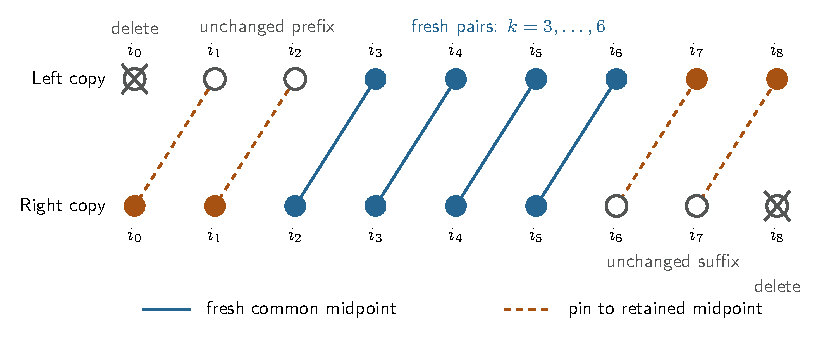
\includegraphics[width=\textwidth]{figures/transport.pdf}
 \caption{The midpoint pairing, shown schematically for $m=8$, $a_0=3$
 and $a_1=5$.  Each link identifies the left midpoint of $i_k$ with the
 right midpoint of $i_{k-1}$.  The middle pairs receive fresh common
 midpoints.  At each end one original trajectory is retained and its
 partner is pinned through the retained midpoint.  After deleting the
 crossed first left and last right tags, all remaining midpoints are
 paired.  The rows show label order, not geometric positions or paths.}
 \label{fig:transport}
\end{figure}

\begin{lemma}[Mass of the transport]\label{long:mass}
For some $c_3>0$, the mass of this common measure satisfies, after averaging
over $(v,w)\in\mathcal A_{K,R}$,
\begin{equation}\label{long:mass-bound}
 \nu_{vw}(1)\ge
       \E[T_v^{\rm rel}T_w^{\rm rel}]-C D^{-1-c_3}-o_K(1).
\end{equation}
\end{lemma}
\begin{proof}
The omitted tags, failed endpoint neighborhoods and route-existence
rejections have total weighted mass $O(D^{-1-c})+o_K(1)$ by
Lemma~\ref{palm:omissions} and Proposition~\ref{rt:routes}.  For the latter
use the marginal bad-site bound in an $O(R^3)$ neighborhood, the
exponentially small probability of a filled component reaching across the
margin, and the thermodynamically vanishing probability of a large
component.  Multiplying by the bounded number of relative-count factors
costs at most $D^{Cx}$, outside events smaller than any power of $D$.

It remains to check the subprobability steps near the two ends.  Use the
full-path count and motion event of Proposition~\ref{lp:good-probability} in the
enlarged endpoint neighborhoods solely to estimate the discarded mass;
it is not added to the conditional bridge law.  Its ordinary-original
motion tests give
$\sup_q|\omega(q)-Y|\le b$ and $\sup_q|\omega(q)-Z|\le b$ in the
chosen lift.  In particular its midpoint $y$ has distance at most $b$
from the source mean.  Consecutive means have distance bounded by a fixed
constant, which is at most $b$ after increasing the fixed cutoff constant.
Thus every required pin has $|y-m_{\rm insert}|\le2b<8b$.
The full-path event fails with weighted mass smaller than $D^{-1-c}$
after the $O(R^3)$ union bound.
On this event, a pinned trial with a separated midpoint has probability at
least $3/4$.  Indeed, start with the full original obstacle collection in
Proposition~\ref{lp:insertion}, delete any replaced originals, and add the
already generated paths.  Only boundedly many added paths can meet the
trial neighborhood, by simplicity of the route.  The last assertion of
that lemma applies to these additions.

For a middle path the necessary separation from a later pinned midpoint
was already checked in the copy containing the retained original that
provides that midpoint.  The paired middle paths have the same midpoint.
The two silent ends are separated by a distance of order $K$, so no check
joins them for sufficiently large $K$.  Thus the only remaining separation
failure is that a selected silent original has midpoint within $s$ of
another original midpoint.  In each bounded region the expected number
of such ordered pairs is at most $CD^2s^3$.  Summing the selected interior
labels uses \eqref{long:label-atom}; summing an end tag uses its factor
$T_v^{-1}$ or $T_w^{-1}$.  Enlarging all site sums to the endpoint
neighborhoods and using the other relative-count bounds gives at most
\[
 C R^3D^{Cx}\frac{D^2s^3}{Df_0}
       \le C D^{-7/5+3w+C'x}.
\]
The midpoint range failure is already covered by the displacement cutoffs
chosen above.  Outside these discarded events every pin has $p\ge3/4$,
so \eqref{long:pin-divisor} equals $p$ and the pin kernel has mass one.
Since $w$ and then $x$ were chosen small, all displayed losses have a
strict power saving beyond $D^{-1}$.  This proves the lemma.
\end{proof}

\subsection{Conditional likelihoods and the checks between two transports}

We next prove absolute continuity of the common measure's augmented lifts
and bound their second moments.  Denote the left lift density by
$\ell_{v,w}$.  Its reference has mass $\E T_v^{\rm rel}$, while its
own mass is $\nu_{vw}(1)$.  The mass estimate therefore shows why the
leading term sought for its second moment is
$\E[T_v^{\rm rel}(T_w^{\rm rel})^2]$: in the centered second moment
the three leading terms combine to
\[
 \E[T_v^{\rm rel}(T_w^{\rm rel})^2]
 -2\E[T_v^{\rm rel}T_w^{\rm rel}]+\E T_v^{\rm rel}
 =\E[T_v^{\rm rel}(T_w^{\rm rel}-1)^2].
\]
Lemma~\ref{palm:counts} controls this last expression.  The task below is
to bound the remaining second-moment error independently of route length.

For a fixed route and label
list let $S=\{i_k:k\ge a_0\}$ be the changed labels in the left copy.
The retained first tag $i$ is not in $S$.  Strip its factor $h_{v,i}/T_v$,
but keep the factor $h_{w,j}$ from the original second tag.  Denote the
resulting likelihood by $L_S$.  The division by $T_w$ and all choices
will be averaged at the end.

Here is an explicit integral defining $L_S$.  For fixed outside paths $o$
let $A_S(x;o)$ be the indicator of all reference checks incident to $S$,
including individual cutoffs, and let
\[
 Z_S(o)=\int A_S(x;o)\,\dd B_S(x),\qquad
 B_S=\bigotimes_{l\in S}B_l.
\]
Let $K_S(x,o;\dd z)$ be the subprobability kernel of the complete
two-copy construction, observed only in its changed left coordinates.
Its input $x$ consists of the latent original $S$ paths.  Define the
finite output measure
\begin{equation}\label{long:unnormalized-output}
 M_S(o;\dd z)=\int A_S(x;o)h_{w,j}(x)
                         K_S(x,o;\dd z)\,\dd B_S(x).
\end{equation}
On reference-admissible configurations,
\begin{equation}\label{long:exact-likelihood}
                         L_S(z,o)=\frac{\dd M_S(o)}{\dd B_S}(z).
\end{equation}
To verify this, both the conditional input law and the conditional reference
output law have the same divisor $Z_S(o)$.  It cancels in their likelihood
ratio, as in Lemma~\ref{palm:likelihood}.  Absolute continuity follows from
the ordinary densities of middle outputs and the distinct latent midpoint
sources for pinned left outputs.  A detailed density bound is proved below.

For upper bounds, integrate out all right pins against the silent prefix.
They occur after the middle steps and are subprobability kernels.  The
left suffix pins do not use these right paths.  Removing these right kernels
therefore increases \eqref{long:unnormalized-output}.  In the rest of the
upper-bound argument $K_S$ denotes this enlarged kernel.  This operation
is the reason that meetings confined to two silent prefixes cost nothing.

Fix two route and label choices with the same first tag, with changed sets
$S,T$ and second tags $j,j'$.  Fix the paths outside $U=S\cup T$, at a value
where the regular conditional reference law is defined.  Every statement
until the averaging subsection is uniform in these fixed allowed values.
Let $Z_U$ be the reference normalizer on $U$ relative to $B_U$.

Define the separate $S$ protocol by deleting the old paths indexed by
$T\setminus S$ from its outside obstacles and removing each check against
such a path.  Keep its list of generated transitions unchanged.  In
particular a right middle path keeps the endpoints of its label even when
that label's old trajectory has been deleted as a left obstacle.  Define
the separate $T$ protocol symmetrically.  Use a superscript minus for these
protocols and write $A_S^-,Z_S^-,M_S^-$ for their reference indicator,
reference normalizer and unnormalized output measure.

These separate quantities depend on their own latent and output variables
and on the common fixed outside of $U$.  They do not depend on the other
set's unshared path variables.  The only apparent exception is the first
right middle insertion at the edge of a silent prefix.  Its old trajectory
is retained on the left, but its right insertion uses only the fixed
endpoints; all checks using the old trajectory are among the deleted
outside checks.  The right pins have already been integrated out.
This verifies the asserted independence also at that edge.

We now specify exactly which comparisons can contribute a cost.  Each
reference check between a label of $S\setminus T$ and a label of
$T\setminus S$ is an edge of a finite graph on these two sets.  Each
deleted proposal check gives a second kind of edge: one end records its
generated transition and the other the removed old opponent label.  A
transition has at most two generated paths, one in each copy.  A label
appears as a primary path once and as an auxiliary path at most once.
The fixed confinement radii imply that a check is identically satisfied
unless the associated route sites have distance at most a fixed $r_c$.
For a predecessor or a midpoint source use the neighboring route site.
Increase $r_c$ once to include these bounded displacements.

Let $J$ be the full site-contact count of Proposition~\ref{rt:routes}, and
$J_*$ its contact count between the changed portions from the common end,
with these step neighbors included.  There are at most $CJ_*$ edges in the
graphs just defined, hence at most $CJ$ edges.  Every degree is bounded by
a constant: a simple lattice route contains only boundedly many vertices
in an $r_c$-ball.  The constants in this assertion do not count the route
length.

For a check between distinct labels $l,k$ put
\begin{equation}\label{long:beta}
 \beta_{lk}=b_D\left(1+\frac1{s\vee d(Y_l,Y_k)}
                       +\frac1{s\vee d(Z_l,Z_k)}\right),
 \qquad b_D=\frac{C(\log D)^C}{D}.
\end{equation}
For a pinned trial with midpoint $y$ checked against an old path $X_k$, also
put
\begin{equation}\label{long:midpoint-cost}
                 m(y,X_k)=\frac{b_D}{s\vee d(y,X_k(0))}.
\end{equation}
All compared labels are distinct, even when the sets $S,T$ intersect:
an outside obstacle is never the label currently inserted.  Lemma
\ref{lp:collision} bounds each corresponding collision or uniform-midpoint
separation cost by $C\beta_{lk}$, and a pinned collision by
$C(\beta_{lk}+m(y,X_k))$ when the pin satisfies separation.  Since
$s=D^{-4/5}$, all these costs are at most $CD^{-19/100}$ for large $D$.
Let $B_{ST}$ be the sum of the $\beta$ costs over all affected checks,
with their bounded multiplicities, and let $M_{ST}$ be the corresponding
sum of \eqref{long:midpoint-cost}.  Thus
\begin{equation}\label{long:worst-cost}
      B_{ST}+M_{ST}\le C D^{-19/100}J.
\end{equation}

\subsection{Reference normalizers and proposal probabilities}

There are two different sources of cost in the product of likelihoods.
Checks between distinct labels prevent the two conditional integrals from
factoring; the next two lemmas compare the reference normalizers and the
proposal probabilities when these checks are removed.  If a label belongs
to both changed sets, its output coordinate is also shared by the two
likelihoods.  We will treat those coordinates separately, by bounding
selected output marginals.

The normalization calculation uses one-path insertion bounds even when
the number of changed paths is large.  No joint normalizer is bounded
below by a constant independent of that number.

\begin{lemma}[Reference normalizers]\label{long:normalizers}
If $S\cap T=\varnothing$, then
\begin{equation}\label{long:disjoint-normalizers}
       1\le\frac{Z_S^-Z_T^-}{Z_U}
                    \le \exp(CB_{ST}).
\end{equation}
If $q=|S\cap T|$ is arbitrary, then
\begin{equation}\label{long:shared-normalizers}
       \frac{Z_S^-Z_T^-}{Z_U}
                    \le C^q\exp(CB_{ST}).
\end{equation}
All normalizers are strictly positive.  In the disjoint case, if $H$ is
any measurable function of the latent originals with $0\le H\le1$, and
$A^- = A_S^- A_T^-$, then
\begin{equation}\label{long:tag-integral-difference}
 0\le \frac1{Z_U}\int H(A^- - A_U)\,\dd B_U
                       \le C e^{CB_{ST}} B_{ST}.
\end{equation}
\end{lemma}
\begin{proof}
The conditional distribution of any one original path, given all the
others, is bounded by $c_0^{-1}B_l$ with $c_0=3/4$, by
Proposition~\ref{lp:insertion}.  This remains true after arbitrary checks have
been removed.  Every reduced normalizer is positive by inserting its
coordinates successively; the resulting lower bound may depend on their
number and is used only for positivity.

Suppose first that $S,T$ are disjoint.  With their cross checks removed the
integral factorizes as $Z_S^-Z_T^-$.  Add the cross checks in any fixed
order.  For a check between $l$ and $k$, condition on all paths except
$l$.  Its failure probability is at most $c_0^{-1}\beta_{lk}$.
Consequently this insertion multiplies the inverse normalizer by at most
\[
 (1-c_0^{-1}\beta_{lk})^{-1}
                         \le \exp(2c_0^{-1}\beta_{lk})
\]
for large $D$.  Multiplication gives
\eqref{long:disjoint-normalizers}.  Under the normalized product with all
cross checks deleted, their union fails with probability at most
$c_0^{-1}\sum\beta_{lk}$.  Dropping $H\le1$ and using the normalizer
ratio proves \eqref{long:tag-integral-difference}.

For general $S,T$, put $A=S\cap T$.  Delete the labels of $A$ and their
incident checks from both separate reference integrals.  This increases
$Z_S^-$ and $Z_T^-$.  The remaining sets $S\setminus A,T\setminus A$
are disjoint, so the preceding comparison applies to them.  Their joint
normalizer is at most $c_0^{-q}Z_U$, since one can add the $q$ labels in
$A$ using their uniform insertion lower bounds.  The cross-check costs
used for the disjoint remainder are among those in $B_{ST}$.  These two
inequalities prove \eqref{long:shared-normalizers}.
\end{proof}

\begin{lemma}[Comparison of transition factors]\label{long:transitions}
Use the same latent originals and the same generated variables in the
original and separate protocols.  The original integrand is bounded by
the separate integrand times a nonnegative factor $\mathcal R$ satisfying
\begin{align}
 \mathcal R&\le e^{C D^{-19/100}J},
                                  \label{long:factor-exponential}\\
 \mathcal R&\le 1+C e^{C D^{-19/100}J}(B_{ST}+M_{ST}).
                                  \label{long:factor-increment}
\end{align}
The assertion is for the product of the two protocols as well.  A
transition with no removed check has ratio exactly one.
\end{lemma}
\begin{proof}
Fix the history before one generated pair or pin.  Its proposal law
before checks is unchanged by deletion of outside obstacles.  Let $p$
and $p^-$ be the acceptance probabilities with and without the removed
checks; then $p\le p^-$.  For a middle pair $p\ge1/2$, and hence
\[
             \frac{p^-}{p}\le 1+2(p^- -p).
\]
For a pin, use $w=\max(1/2,p)$ and $w^- =\max(1/2,p^-)$.  The map
$p\mapsto\max(1/2,p)$ is increasing and $1$-Lipschitz, so
\[
             \frac{w^-}{w}\le 1+2(p^- -p).
\]
The ratio of admissibility indicators is bounded by one in this upper
comparison.  A midpoint separation indicator outside the pin proposal
can also be increased.  On the support of the old nonzero integrand, its
midpoint is separated from every old opponent, so the pinned collision
estimate applies.  Off that support the inequality is automatic.  The
capped expression \eqref{long:midpoint-cost} thus gives a valid bound
everywhere.

For a middle proposal the union bound gives
$p^- -p\le C\sum\beta_{lk}$ over its removed checks.  For a pin the
bound is $C\sum(\beta_{lk}+m(y,X_k))$.  The proposal may be a coupled
pair, but the removed checks involve one of its two marginals, and the
uniform-midpoint insertion bounds apply to those marginals.  Conditioning
the original proposal does not enter this estimate of $p^- -p$.

Multiplying the displayed ratio bounds over the affected transitions of
both protocols gives
$\mathcal R\le\exp(C(B_{ST}+M_{ST}))$.
The inequalities $e^a-1\le ae^a$ and
\eqref{long:worst-cost} give both conclusions.  Unaffected transitions
have identical numerators and divisors at the same history.  Thus the
number of factors actually paid is bounded by the number of graph edges,
not by the number of generated transitions.
\end{proof}

\subsection{Marginals of selected output paths}

Before multiplying likelihoods with shared labels, we record the precise
form of reverse integration used for their common output coordinates.
Only primary marginals of a coupled pair are bounded.  Its full two-copy
law has equal midpoints and is not dominated by a product of free bridges.

\begin{lemma}[Selected outputs of sequential kernels]\label{long:kernel}
Let $\mu(\dd x)$ be a probability measure of latent variables, followed by
a finite ordered list of subprobability kernels.  At stage $r$ the kernel
generates a primary variable $z_r$ and arbitrary auxiliary variables.  Let
$Q$ be a set of stages.  Suppose that, for every latent input and every
allowed preceding history, the primary marginal at $r\in Q$ is at most
$A_r\nu_r(x,\dd z_r)$, where $\nu_r$ is a subprobability kernel depending
on $x$ but not on the preceding history.  Then the joint measure of the
selected primary outputs is at most
\begin{equation}\label{long:reverse-kernel}
       \left(\prod_{r\in Q}A_r\right)
                   \int\mu(\dd x)\prod_{r\in Q}\nu_r(x,\dd z_r).
\end{equation}
\end{lemma}
\begin{proof}
Integrate an arbitrary nonnegative measurable test function of the selected
outputs.  Starting with the last stage, integrate every unselected stage
using its mass bound one.  At a selected stage integrate its auxiliary
variables and use the primary marginal bound.  The new test function
depends on the latent input and the earlier selected outputs, but no
longer on the history variables generated at this stage.  Induction
backwards through the finite list proves \eqref{long:reverse-kernel}.
The argument first applies to bounded tests and then to all nonnegative
tests by monotone convergence.
\end{proof}

\begin{lemma}[Uniform marginal bound]\label{long:shared-density}
Divide the separate output measure $M_S^-$ by its reference normalizer
$Z_S^-$, and omit its original tag indicator if desired.  For any $q$
specified primary output labels, its marginal is dominated by
\begin{equation}\label{long:marginal-bound}
                 G_D^q\bigotimes_{l\text{ specified}} B_l,
              \qquad G_D=C D^{C\sqrt x}.
\end{equation}
The same assertion holds for $T$, and the constants are independent of
the number of unselected outputs.
\end{lemma}
\begin{proof}
The normalized separate latent-original law is its admissible product
bridge law.  A middle stage, conditional on all these originals and on
the preceding history, has primary marginal at most
$C D^{Cx}B_l$, by Corollary~\ref{lp:trial-density} and its acceptance
probability at least $1/2$.  A pin has primary conditional bridge law at
most $2\1_{\rm range}(y) B_l(\dd z\mid z(0)=y)$, where $y$ is the
midpoint of its retained original partner and
$\1_{\rm range}(y)=\1_{\{|y-m_l|\le8b\}}$; all separation and avoidance
indicators are discarded in this upper bound, so the retained cutoff is
independent of the preceding history.  This cutoff conditional bridge is
the kernel $\nu_r$ in Lemma~\ref{long:kernel}.  Both estimates hold
uniformly in the history, including
histories obtained after deleting some outside checks.

Apply Lemma~\ref{long:kernel} to the specified stages.  For each specified
pin its source is a latent original in $S$: these sources lie in the
right-silent suffix.  The sources for distinct pins are distinct labels.
If there are $p$ specified pins, their joint latent-source marginal is
bounded by $C^p$ times the corresponding product bridge law, by
Corollary~\ref{lp:trial-density}.  Indeed the uniform conditional one-path
density bound survives integration over any other latent coordinates and
can then be iterated over these $p$ coordinates.

Let $a(l)$ be the source label of the pin with output label $l$.  Integrating
out all parts of its source other than the midpoint gives
$g_{a(l)}(y)\,\dd y$.  On the retained range, neighboring means and
the Gaussian ratio bound~\eqref{lp:midpoint-ratio} give
$g_{a(l)}(y)\le C D^{C\sqrt x}g_l(y)$.  Therefore
\[
 \int \1_{\rm range}(y)g_{a(l)}(y)
           B_l(\dd z\mid z(0)=y)\,\dd y
                         \le C D^{C\sqrt x}B_l(\dd z).
\]
Use this for each distinct source.  Together with the middle-output
bounds it proves \eqref{long:marginal-bound}.  No assertion of independence
between a pin and its source midpoint has been used: the midpoint is
integrated against the conditional bridge before the resulting free
bridge bound is obtained.
\end{proof}

\subsection{The product of two likelihoods}

\begin{lemma}[Disjoint and shared changed sets]\label{long:product}
At almost every fixed admissible outside of $U=S\cup T$, the likelihoods
of the two original transports satisfy the following bounds.  If $S,T$
are disjoint, then
\begin{equation}\label{long:disjoint-product}
 \E[L_SL_T\mid U^c]\le
 \E[h_{w,j}h_{w,j'}\mid U^c]
 +C e^{C D^{-19/100}J}
          \bigl(B_{ST}+J_*b_D(1+t^{-3/2})\bigr).
\end{equation}
If $q=|S\cap T|\ge1$, then
\begin{equation}\label{long:shared-product}
          \E[L_SL_T\mid U^c]
                     \le e^{C D^{-19/100}J}G_D^q,
\end{equation}
after increasing the fixed constant in $G_D$.
\end{lemma}
\begin{proof}
By \eqref{long:exact-likelihood} and the enlargement of the kernels, the
conditional product integral is bounded by the integral using
the free output measure $B_U$, the union admissibility indicator, and the
single divisor $Z_U$.  In each likelihood keep a separate set of latent
original variables.  These copies are not identified even if $S,T$ have
common labels.  Only shared output coordinates are identified by the
integration against $B_U$.

Suppose first that the sets are disjoint.  Apply Lemma
\ref{long:transitions}, delete the union output-admissibility indicator in
an upper bound, and integrate with the separate protocols.  The term one
in \eqref{long:factor-increment} has integral at most
\[
 \frac1{Z_U}
       \int A_S^-(x)A_T^-(x')h_{w,j}(x)h_{w,j'}(x')
                              \,\dd B_S(x)\dd B_T(x').
\]
Here the generated kernels were integrated using their mass bounds one.
By \eqref{long:tag-integral-difference} this is at most the reference
expectation of $h_{w,j}h_{w,j'}$, plus
$Ce^{CB_{ST}}B_{ST}$.  The terms from $B_{ST}$ in
\eqref{long:factor-increment} are bounded by the same normalizer ratio
and the masses of the separate normalized protocols, each at most one.

Consider one term $m(y,X_k)$ of $M_{ST}$.  Its midpoint $y$ belongs to
a latent original of one separate protocol, whereas $X_k$ is an output
path of the other.  Conditional on the fixed outside the two extended
protocol measures are independent.  On the side providing $y$, drop its
tag indicator and integrate all generated transitions.  The marginal of
the source original is bounded by a fixed constant times its free bridge.
For every fixed point $z$, the Gaussian midpoint density then gives
\begin{align*}
 \int_{d(y,z)\le C_b}\frac{g_l(y)}{s\vee d(y,z)}\,\dd y
 &\le \|g_l\|_\infty\int_{|u|\le1}|u|^{-1}\,\dd u
            +\int_{d(y,z)>1}g_l(y)\,\dd y\\
 &\le C(1+t^{-3/2}).
\end{align*}
The local range $C_b$ suffices because all other checks vanish; nearby
lifts or the periodized Gaussian give the same estimate.  This calculation
does not require a density bound for the opposing output midpoint.
There are at most $CJ_*$ such terms.  Use
\eqref{long:disjoint-normalizers} for the normalizer ratio and absorb its
exponent using \eqref{long:worst-cost}.  This proves
\eqref{long:disjoint-product}.

For intersecting sets use \eqref{long:factor-exponential}.  After dropping
union admissibility, write the separate output measures as $Z_S^-f_S B_S$
and $Z_T^-f_T B_T$, with the original tag indicators included.  Integrating
unshared output coordinates leaves the product of their marginals on
$A=S\cap T$.  By Lemma~\ref{long:shared-density}, one of these marginal
densities is at most $G_D^q$; the other has integral at most one.  Thus the
free output integral is at most $Z_S^-Z_T^-G_D^q$.  Division by $Z_U$,
\eqref{long:shared-normalizers}, and absorption of $C^q$ in $G_D^q$
prove \eqref{long:shared-product}.
\end{proof}

\subsection{Averaging labels, routes and endpoints}

We now return to the original augmented reference and its left lift
density $\ell_{v,w}$.  It is zero on omitted first tags or rejected data.
On retained data and
first tag $i$ it is the sum of $L_S/T_w$ over the candidate second tags,
averaged over the route and interior-label choices.  Squaring this sum
produces exactly two independent choices with common first tag $i$ and
the same underlying data.  In particular the data are never independently
resampled when the likelihood is squared.

\begin{lemma}[Endpoint sums and label matches]\label{long:label-average}
At fixed retained data and route sites, the label average of the error in
\eqref{long:disjoint-product}, together with the contribution of all
choices having $S\cap T\ne\varnothing$, is at most
\begin{equation}\label{long:label-error}
                C D^{-1+\zeta(x)}J_*e^{\delta_D J},
             \qquad \delta_D\longrightarrow0,
             \qquad \zeta(x)\longrightarrow0\quad(x\downarrow0).
\end{equation}
This estimate includes the normalized sums over the three tag labels at
their specified mean-sites.  The remaining weight of each tag site is
at most $CR^{-3}$.
\end{lemma}
\begin{proof}
Every possible mean-site of an end tag lies in the corresponding $R$-cell
enlarged by a fixed radius.  At each site the number of eligible tags is
at most $Cf_0D$, by the endpoint count estimate.  Since
$T_v=T_w=f_0DR^3$, their counting sums with $h\le1$ are dominated by a
site weight $CR^{-3}$ and a label subprobability measure with maximum atom
$C/(Df_0)$.  These are deterministic upper bounds at the fixed data;
the site weights will be removed before any environmental expectation.
Zero or very small tag families cause no problem: their extracted label
measure simply has mass less than one.  Interior selections are probability
measures and have the same maximum-atom bound
\eqref{long:label-atom}.

For any fixed endpoint $z$, a dyadic decomposition of the endpoint count
bound in Definition~\ref{lp:certificate} gives, for a candidate label family
in a bounded neighborhood,
\begin{equation}\label{long:endpoint-average}
 \frac{C}{Df_0}\sum_l\frac1{s\vee d(z,Y_l)}
          \le C\left(1+\frac{D^{1/100}}{Df_0s}\right)\le C,
\end{equation}
and the same holds for the $Z$ endpoints.  To see the first inequality,
sum separately the innermost ball of radius $s$ and the shells
$2^as<d\le2^{a+1}s\le C_b$.  The volume term sums as a geometric
series of order $Df_0$, whereas the additive $D^{1/100}$ term sums to
$CD^{1/100}/s$.  Here $D^{1/100}/(Df_0s)=D^{-19/100+x}$ is bounded
for small $x$.

Every edge contributing a $\beta$ cost has a label choice on at least one
side which is free to average: the common first tag is outside both changed
sets.  For an interior label use \eqref{long:endpoint-average} conditional
on the tags; for an end-tag label use the same bound in its candidate
family at its fixed mean-site.  Coincidence exclusions may be removed in
this positive upper bound, because the reciprocal distance is capped at
$s$.  Thus each averaged $\beta$ costs at most $Cb_D$, and there are at
most $CJ_*$ edges.  The midpoint cost in
\eqref{long:disjoint-product} has already been integrated.  This bounds
the disjoint error by
\[
       C e^{C D^{-19/100}J}J_*b_D(1+t^{-3/2}).
\]

For the intersecting choices let $\mathcal E$ be all pairs of slots in
the two changed lists whose label choices could agree.  Its cardinality
is at most $CJ_*$, with all such pairs among the $CJ$ full contacts.
Because each list has distinct labels, the actual matches form a matching:
no slot belongs to two of them.  The product label measure assigns each
prescribed set of $h$ disjoint matches mass at most $(C/(Df_0))^h$.
For interior matches,
this follows by conditioning on the tags and then on one list, and using
independence between sites in the other list.  A tag can match an interior
slot only at its one possible base site.  For a match of the two second
tags, sum one tag with the same maximum-atom bound.  There are only two
noncommon tag slots, so their exclusions change these bounds by a fixed
factor per prescribed match, independent of the route length.

The tag measures have mass at most one, so summing the remaining tag
variables cannot increase this bound.

Expand
\[
 G_D^q=\prod_{e\in\mathcal E}
             \bigl(1+(G_D-1)\1_{\{e\ {\rm matched}\}}\bigr).
\]
To restrict to at least one match, designate one matched edge and bound
the remaining product in the same way.  The preceding probability bound
and the elementary inequality $(1+a)^M\le e^{aM}$ give
\begin{equation}\label{long:match-sum}
 \E_{\rm labels}[\1_{\{q>0\}}G_D^q]
       \le \frac{C G_D}{Df_0}J_*
                         \exp\left(\frac{C G_D}{Df_0}J\right).
\end{equation}
Use this in \eqref{long:shared-product}.  Since
$G_D/(Df_0)=C D^{-1+x+C\sqrt x}$, the coefficient in this last
exponent tends to zero.  Absorb the fixed powers of $\log D$ in an
arbitrarily small power depending on $x$, and combine the two estimates.
They have the form \eqref{long:label-error}, with for example
$\delta_D=C D^{-19/100}+C G_D/(Df_0)$.  This proves the lemma.
\end{proof}

The next step is the only place where the environment is averaged in the
likelihood estimate.  The two routes share that environment.  For each
deterministic common endpoint, Proposition~\ref{rt:routes} supplies
\[
 \E[\1_{\rm retained}e^{\kappa J}]\le C,
 \qquad
 \E_{\rm sites}\E[\1_{\rm retained}\1_{\{J_*>0\}}]
                                                \le CR^{-c_g}.
\]
The second average is over the two independent noncommon sites with
weights at most $CR^{-3}$ each.  The deterministic bounds in
Lemma~\ref{long:label-average} allow precisely this site average even
though the actual candidate tag counts depend on the environment.
For large $D$, $J^2e^{2\delta_DJ}\le C_\kappa e^{\kappa J}$.
As $J_*\le J$, Cauchy--Schwarz consequently gives
\begin{equation}\label{long:route-average}
 \E_{\rm sites}\E[
     \1_{\rm retained}J_*e^{\delta_DJ}]
                      \le C R^{-c_g/2}.
\end{equation}
Uniformity in the common endpoint permits its remaining average as well.
Combining \eqref{long:label-error} and \eqref{long:route-average} bounds
the averaged likelihood error by
$C D^{-1+\zeta(x)-wc_g/2}$.  Choose $x$ small enough that
$\zeta(x)<wc_g/4$.  This has a strict power saving beyond $D^{-1}$.

\begin{proposition}[Augmented moments]\label{long:augmented-moments}
For some $c_4>0$, the left augmented likelihood satisfies
\begin{equation}\label{long:second-moment}
 \int\ell_{v,w}^2\,\dd P_{{\rm aug},v}
       \le \E[T_v^{\rm rel}(T_w^{\rm rel})^2]
                           +CD^{-1-c_4}+o_K(1)
\end{equation}
after averaging over $\mathcal A_{K,R}$.  Its mass satisfies
\eqref{long:mass-bound}, and the same estimates hold with $v,w$ exchanged.
\end{proposition}
\begin{proof}
In the expansion of the squared likelihood keep the common first-tag
factor $h_{v,i}/T_v$.  Conditional on the outside of $S\cup T$ it is
fixed, because neither changed set contains $i$.  Apply
Lemma~\ref{long:product} to the two choices.  The conditional expectation
in its disjoint leading term is exactly the original expectation of the
two end-tag indicators.  All tag choices, route choices, and interior
label choices are fixed independently of the latent paths, conditional
on the data.  We may therefore sum this leading term on the original
path space.  Removing all good-event and noncoincidence restrictions in
this nonnegative upper bound yields
\[
 \E\left[
    \left(\sum_i\frac{h_{v,i}}{T_v}\right)
    \left(\sum_j\frac{h_{w,j}}{T_w}\right)^2\right]
             =\E[T_v^{\rm rel}(T_w^{\rm rel})^2].
\]
The errors and intersecting choices are controlled by
Lemma~\ref{long:label-average} and \eqref{long:route-average}.  This
proves \eqref{long:second-moment}.  The mass bound is
Lemma~\ref{long:mass}.  For the right augmented estimate keep the same
two-copy construction, and hence the same common measure.  Reverse only
the list indexing and designate the right copy primary; retain the actual
chronological order of the generated middle kernels.  Its common endpoint
is then the last tag and its silent prefix is the previous silent suffix.
The kernels pinned into the left copy can now be integrated out.  The
remaining right pins do not use them: the two end families lie in opposite
copies, and no check joins the separated endpoint neighborhoods.  Every
kernel estimate and the reverse-integration lemma hold for an arbitrary
fixed middle order, so this change of designation requires no resampling
or reversal of the sampling order.

The original retention also gives the event required for the reversed
route comparison.  The fixed endpoint cube $Q_v$ and its $10R$ margin
are bad-free.  For every filled bad component, the actual first endpoint
lies outside its fill by the original route event.  Since $Q_v$ is
nearest-neighbor connected and contains that endpoint, a path in $Q_v$
cannot enter the fill without meeting the bad component.  Thus every site
of $Q_v$ lies outside every such fill.  The component-size cutoff is
unchanged, so Proposition~\ref{rt:routes} applies with the common terminal
endpoint and the noncommon endpoints in $Q_v$.
The preceding calculation therefore gives the right augmented estimates
for the original common measure.
\end{proof}

\begin{proof}[Proof of Proposition~\ref{long:comparison}]
The augmented reference has mass $\E T_v^{\rm rel}$, while its common
measure has mass $\int\ell_{v,w}\,\dd P_{{\rm aug},v}$.  Subtract twice
the mass lower bound from the second-moment upper bound and add the
reference mass.  Proposition~\ref{long:augmented-moments} gives
\begin{equation}\label{long:centered-second}
 \int|\ell_{v,w}-1|^2\,\dd P_{{\rm aug},v}
 \le \E[T_v^{\rm rel}(T_w^{\rm rel}-1)^2]
                                      +o(D^{-1})+o_K(1)
\end{equation}
in the normalized pair average.  The likelihood remains zero on the
omitted reference events; their loss was included in the mass estimate.

Outside the negligible count tails, $T_v^{\rm rel}\le C/f_0$.
Lemma~\ref{palm:counts} and the uniform marginal weights of the ordered
cell pairs therefore bound the main term of
\eqref{long:centered-second} by
\[
 C D^x\bigl(D^{-1-w/6}+D^{-1+x}R^{-3}\bigr)
     \le C\bigl(D^{-1-w/6+x}+D^{-1+2x-3w}\bigr)
                                      =o(D^{-1}).
\]
The removed count tails remain negligible after multiplication by the
relative counts, by the bookkeeping in Lemma~\ref{palm:counts}.  Choose
$x<w/12$, in addition to its preceding restrictions.  The same centered
bound holds in the right augmented reference.

For finite measures $P$ and $\nu\ll P$ with likelihood $\ell$, their
squared Hellinger distance is
$\int(1-\sqrt\ell)^2\,\dd P\le\int(1-\ell)^2\,\dd P$.
Projection cannot increase this distance: conditional Cauchy--Schwarz
increases the affinity and preserves both masses.  Project both augmented
comparisons to the common ordered bath.  Their reference densities are
$s_v^2$ and $s_w^2$, by Lemma~\ref{palm:reference}, and their
common projected density is that of $\nu_{vw}$.  The triangle inequality
in $L^2$ and the two bounds \eqref{long:centered-second} now imply
\eqref{long:hellinger}.  Every volume-dependent rejection was recorded
as $o_K(1)$ at fixed dilution; taking that limit before $D\to\infty$
completes the assertion.
\end{proof}

\section{Control of long-wavelength excitations}\label{asm:section}\label{sec:assembly}

The local energy estimate controls excitations outside the space of
functions constant on $R$-cells. We now use the two deletion comparisons
to show that the remaining excitations, between that space and the single
constant orbital, have density $o(1)$. The distant comparison makes cell
root-mean-squares nearly constant; the local fourth-moment comparison
relates those root-mean-squares to cell averages. This gives the estimate
needed to pass from local observables to global momentum tests.

\subsection{A variance bound from distant pairs}

We first remove the restriction on the pairs of $R$-cells in
Proposition~\ref{long:comparison}. This is a statement about arrays in
a Hilbert space and has no ground-state assumption.

\begin{lemma}[Distant pairs control the variance]\label{asm:far-pairs}
Let $\mathcal H$ be a complex Hilbert space and let
$f_z\in\mathcal H$, $z\in(\Z/M\Z)^3$. Set
\[
 I_M=\{h\in\{0,\ldots,M-1\}:.30M\le h\le .45M\},
 \qquad \overline f=M^{-3}\sum_z f_z.
\]
For all sufficiently large $M$, there is an absolute constant $C$ such
that
\begin{equation}\label{asm:far-variance}
 \frac1{M^3}\sum_z\|f_z-\overline f\|_{\mathcal H}^2
 \le \frac{C}{M^3|I_M|M^2}
      \sum_z\sum_{h_1\in I_M}\sum_{h_2,h_3\in\Z/M\Z}
             \|f_{z+h}-f_z\|_{\mathcal H}^2.
\end{equation}
\end{lemma}

\begin{proof}
Use the unitary discrete Fourier transform on $(\Z/M\Z)^3$.
The right-hand quadratic form before multiplication by $C$ has Fourier
multiplier
\[
 a_M(k)=\frac1{|I_M|M^2}
   \sum_{h_1\in I_M}\sum_{h_2,h_3}
       |e^{2\pi i k\cdot h/M}-1|^2.
\]
The variance on the left has multiplier one for $k\ne0$ and zero at
$k=0$, so it suffices to bound $a_M(k)$ below away from zero for $k\ne0$.
If $k_2$ or $k_3$ is nonzero modulo $M$, orthogonality gives $a_M(k)=2$.
Otherwise, write $q=\min(k_1,M-k_1)$. For $q\ge1$, the geometric-sum
formula and $\sin(\pi q/M)\ge2q/M$ give
\[
 \left|\frac1{|I_M|}\sum_{h\in I_M}e^{2\pi i k_1h/M}\right|
        \le \frac{C_0}{q}.
\]
Thus $a_M(k)\ge1$ when $q\ge2C_0$. For each of the finitely many
remaining positive $q$, the common value
$a_M(q,0,0)=a_M(M-q,0,0)$ converges to
\[
 \frac1{.15}\int_{.30}^{.45}|e^{2\pi i q t}-1|^2\,\dd t>0.
\]
Their minimum is positive, uniformly for large $M$. Parseval's identity
now proves \eqref{asm:far-variance}, including Hilbert-valued arrays.
\end{proof}

For a fixed nonnegative ground vector $\Phi$ and a cell
$A\in\mathcal C_d\cup\mathcal C_R$, the function $s_A$ of
Lemma~\ref{palm:reference} belongs to
$\mathcal H=L^2(\Lambda_K^{N-1},\dd Y)$. Explicitly,
\begin{equation}\label{asm:rms}
 s_A(Y)=\left(\frac V{|A|}\int_A\Phi(y,Y)^2\,\dd y\right)^{1/2}.
\end{equation}
Applying Lemma~\ref{asm:far-pairs} with $M=K/R$ to
Proposition~\ref{long:comparison} gives
\begin{equation}\label{asm:rms-variance}
 \frac1{|\mathcal C_R|}\sum_{A\in\mathcal C_R}
    \left\|s_A-\frac1{|\mathcal C_R|}\sum_{A'}s_{A'}\right\|_2^2
       =o(D^{-1})+o_K(1).
\end{equation}
The uniformity and order of limits are those of
Section~\ref{set:section}.

\subsection{From root-mean-squares to arithmetic means}

The occupation involves an integral of $\Phi$, whereas $s_A$ is a
root-mean-square of $\Phi$. The next elementary inequality explains why
the fourth-moment local comparison is enough to bridge this difference.

\begin{lemma}[RMS interpolation]\label{asm:rms-interpolation}
For any finite nonempty array of nonnegative numbers $y_i$, with uniform
averaging denoted by $\mathbb E_i$, put
$a=\mathbb E_i y_i^2$ and $m=\mathbb E_i y_i$. Then
\begin{equation}\label{asm:rms-inequality}
 (\sqrt a-m)^2\le\frac12\mathbb E_{i,i'}
           \frac{(y_i-y_{i'})^4}{y_i^2+y_{i'}^2}.
\end{equation}
The quotient is defined to be zero when its denominator is zero.
Furthermore, for every $y,z\ge0$,
\begin{equation}\label{asm:sqrt-comparison}
 |\sqrt y-\sqrt z|^4
 \le\frac{(y-z)^4}{y^2+z^2}
 \le8|\sqrt y-\sqrt z|^4.
\end{equation}
\end{lemma}

\begin{proof}
Let $Q$ denote the double average on the right of
\eqref{asm:rms-inequality}, before its factor $1/2$. Weighted
Cauchy--Schwarz and independence of the two uniform indices give
\[
 [2(a-m^2)]^2
 =\bigl[\mathbb E_{i,i'}(y_i-y_{i'})^2\bigr]^2
 \le Q\mathbb E_{i,i'}(y_i^2+y_{i'}^2)=2aQ.
\]
If $a>0$, divide by $4(\sqrt a+m)^2\ge4a$; the case $a=0$ is
immediate. For the second statement factor
$y-z=(\sqrt y-\sqrt z)(\sqrt y+\sqrt z)$. The remaining ratio is
$(\sqrt y+\sqrt z)^4/(y^2+z^2)$, which lies between $1$ and $8$.
\end{proof}

For any two $d$-cells $z,z'$ write
\[
 Q_{z,z'}(Y)=
   \frac{|s_z(Y)-s_{z'}(Y)|^4}{s_z(Y)^2+s_{z'}(Y)^2}.
\]
For a nearest-neighbor edge $e=(z,z')$, abbreviate this as $Q_e$.
Inside one $R$-cell, any two $d$-cells can be joined by a path of at most
$3R/d$ nearest-neighbor steps that stays in the cell. Put
$t_z(Y)=\sqrt{s_z(Y)}$. If the path has $m$ edges, then
\eqref{asm:sqrt-comparison} and H\"older's inequality give
\[
 Q_{z,z'}\le8|t_z-t_{z'}|^4
       \le8m^3\sum_{e=(v,w)\text{ on the path}}|t_v-t_w|^4
       \le8m^3\sum_{e\text{ on the path}}Q_e.
\]
Enlarging the last sum to all internal edges yields
\begin{equation}\label{asm:path-fourth}
 Q_{z,z'}(Y)\le C_jR^3
       \sum_{e\text{ internal edge of the }R\text{-cell}}Q_e(Y).
\end{equation}
The full internal edge sum bounds every pair, so no estimate of path
multiplicities is needed. Averaging over pairs and over $R$-cells, and using
$|\mathcal C_d|/|\mathcal C_R|=(R/d)^3$, consequently gives
\begin{align}
 &\frac1{|\mathcal C_R|}\sum_{A\in\mathcal C_R}
   \frac1{|\{z\in\mathcal C_d:z\subset A\}|^2}
    \sum_{z,z'\subset A}\int Q_{z,z'}\,\dd Y
 \notag\\
 &\hspace{20mm}\le C_jR^6\,
       \frac1{|\mathcal C_d|}\sum_{e\text{ a nearest-neighbor edge}}
             \int Q_e\,\dd Y
 \notag\\
 &\hspace{20mm}\le C_j R^6 D^{-1-u/8}+o_K(1)
 =o(D^{-1})+o_K(1).
 \label{asm:all-local-pairs}
\end{align}
The second inequality is Proposition~\ref{palm:local-comparison}.
The last uses $6w<u/8$, which follows from \eqref{set:exponents}.
For fixed dilution the factor $R^6$ is fixed, so it causes no difficulty
for the thermodynamic remainder.

Define
\begin{equation}\label{asm:field-means}
 F(y,Y)=\sqrt V\Phi(y,Y),\qquad
 m_A(Y)=\frac1{|A|}\int_A F(y,Y)\,\dd y.
\end{equation}
Spatial integrals of $F$ over the whole torus will use the normalized
measure $\dd y/V$. For each cell, nonnegativity of $F$ implies
$0\le m_A\le s_A$, and
\[
 (s_A-m_A)^2\le s_A^2-m_A^2
       =\frac1{|A|}\int_A|F-m_A|^2\,\dd y.
\]
It follows from \eqref{en:d-occupation} and bosonic symmetry that
\begin{equation}\label{asm:micro-mean-rms}
 \frac1{|\mathcal C_d|}\sum_{z\in\mathcal C_d}
       \|m_z-s_z\|_2^2
 \le\|(W_d)_1\Phi\|_2^2
 =\frac1D\frac1V\langle\mathrm d\Gamma(W_d)\rangle_\Phi
 \le D^{-1}(\epsilon_j+o(1))+o_K(1),
\end{equation}
where $\epsilon_j\to0$ as $j\to\infty$, and the dilute remainder is taken
at fixed $j$.

For an $R$-cell $A$, the number $s_A(Y)$ is the root-mean-square of
the numbers $s_z(Y)$ over its $d$-cells. Let $\overline s_A(Y)$ denote
their arithmetic mean. Lemma~\ref{asm:rms-interpolation} and
\eqref{asm:all-local-pairs} imply
\begin{equation}\label{asm:R-rms-arithmetic}
 \frac1{|\mathcal C_R|}\sum_A\|s_A-\overline s_A\|_2^2
           =o(D^{-1})+o_K(1).
\end{equation}
Also $m_A$ is the arithmetic mean of the $m_z$ in $A$. Jensen's
inequality, \eqref{asm:micro-mean-rms}, and
\eqref{asm:R-rms-arithmetic} therefore give
\begin{equation}\label{asm:R-mean-rms}
 \frac1{|\mathcal C_R|}\sum_A\|m_A-s_A\|_2^2
       \le D^{-1}(2\epsilon_j+o(1))+o_K(1).
\end{equation}

\subsection{The infrared estimate and arbitrary ground vectors}

\begin{proposition}[Remaining excitations]\label{asm:infrared}
Put $Q_R=P_R-P_0$. Uniformly over normalized, possibly complex,
bosonic ground vectors,
\begin{equation}\label{asm:infrared-bound}
 D\|(Q_R)_1\Phi\|_2^2\le16\epsilon_j+o(1)+o_K(1),
\end{equation}
where $\epsilon_j\to0$. The coefficient $16$ is independent of $j$;
the dilute remainder may depend on $j$. The exponents $u,w$ and the scale $R$ may be
kept fixed when $j$ is increased; all dilute and volume thresholds may
depend on $j$.
\end{proposition}

\begin{proof}
First let $\Phi\ge0$. For Hilbert-valued arrays, the variance is the
minimum of the mean squared distance to a constant array. Comparing the
array $m_A$ with the mean of the array $s_A$ thus yields
\[
 \frac1{|\mathcal C_R|}\sum_A\|m_A-\overline m\|_2^2
 \le\frac2{|\mathcal C_R|}\sum_A\|m_A-s_A\|_2^2
      +\frac2{|\mathcal C_R|}\sum_A\|s_A-\overline s\|_2^2.
\]
Here bars without cell subscripts denote averages over all $R$-cells.
The left side is exactly $\|(P_R-P_0)_1\Phi\|_2^2$, by
\eqref{asm:field-means} and the normalized spatial measure.
Equations~\eqref{asm:rms-variance} and \eqref{asm:R-mean-rms} prove
\eqref{asm:infrared-bound} for nonnegative vectors, with coefficient $4$
in place of $16$. The multiplication
of a volume remainder by $D$ is harmless in the inner limit because
$D\to D_*$.

For a real bosonic ground vector $f$, its positive and negative parts
$f_+,f_-$ belong to the Dirichlet form domain and remain symmetric.
The Sobolev truncation identities give
\[
 \|f\|_2^2=\|f_+\|_2^2+\|f_-\|_2^2,
 \qquad q[f]=q[f_+]+q[f_-].
\]
Each nonzero part has Rayleigh quotient at least $E_N$, and their sum
attains $E_N$. Both nonzero parts therefore attain $E_N$ and are ground
vectors. Complex conjugation commutes with the operator, so the real
and imaginary parts of a complex ground vector are ground vectors or
zero. A normalized $\Phi$ can consequently be written as
\[
 \Phi=\sum_{a=1}^m c_a\Phi_a,
 \qquad m\le4,\quad \Phi_a\ge0,\quad\|\Phi_a\|_2=1,
 \qquad \sum_{a=1}^m|c_a|^2=1,
\]
where each $\Phi_a$ is a ground vector. Cauchy--Schwarz gives
\[
 \|(Q_R)_1\Phi\|_2^2
       \le\sum_{a=1}^m\|(Q_R)_1\Phi_a\|_2^2.
\]
Thus at most a factor four is lost in the vanishing error in
\eqref{asm:infrared-bound}. No comparison of component phases or
connectedness assumption is used.
\end{proof}

Because $P_0\le P_R$, $Q_R$ and $W_R$ are orthogonal projections with
\begin{equation}\label{asm:orthogonal-decomposition}
 1-P_0=W_R+Q_R.
\end{equation}
Consequently every normalized bosonic ground vector satisfies the exact
identity
\begin{equation}\label{asm:depletion-decomposition}
 D(1-B(\Phi))=
        \frac1V\langle\mathrm d\Gamma(W_R)\rangle_\Phi
                   +D\|(Q_R)_1\Phi\|_2^2.
\end{equation}
We record the conclusions in the per-volume normalization used for
momentum observables:
\begin{align}
 \frac1V\langle\mathrm d\Gamma(P_R-P_0)\rangle_\Phi
   &=D\|(P_R-P_0)_1\Phi\|_2^2=o(1),
       \label{asm:coarse-density}\\
 \frac1V\langle\mathrm d\Gamma(1-P_0)\rangle_\Phi
   &=D(1-B(\Phi))=\cD\alpha^{3/2}+o(1).
       \label{asm:scaled-depletion}
\end{align}
Both remainders are uniform over normalized, possibly complex ground
vectors in the iterated limit of Section~\ref{set:section}. For the first,
bosonic symmetry gives the equality, and Proposition~\ref{asm:infrared}
gives the error estimate: choose $j$ large and then increase the lower
bound on $D$ and the volume threshold. The left side is independent of
$j$, since $u,w,R$ remain fixed. The second follows from
\eqref{asm:depletion-decomposition} and \eqref{en:R-occupation}, whose
energy estimate applies directly to complex ground vectors.

\section{From local covariances to the momentum distribution}
\label{mom:section}\label{sec:momentum}

The local covariance estimate describes one-body operators inside a
$B$-box, whereas momentum occupation is defined by Fourier modes on the
whole torus. Translations connect these two descriptions: their
expectations are the Fourier transform of the momentum measure. We
first remove the remaining cell-constant excitations, then average the
position of the $B$-box boundaries. This makes the cost of cutting a
translation small compared with the excitation count.

\subsection{Translations and shifted box boundaries}

For a normalized ground vector $\Phi$ on $\Lambda_K$, put
$u_{p,K}(y)=V^{-1/2}e^{ip\cdot y}$ and define the positive momentum measure
\begin{equation}\label{mom:scaled-measure}
 \mathfrak m_\Phi
   =\frac1V\sum_{\substack{p\in(2\pi/K)\Z^3\\p\ne0}}
       \langle u_{p,K},\gamma^{(1)}_\Phi u_{p,K}\rangle\,\delta_p.
\end{equation}
Here $\gamma^{(1)}_\Phi$ is the one-particle density matrix of $\Phi$ and
$\delta_p$ is unit mass at $p$. Let $T_hg(y)=g(y+h)$ for $h\in\R^3$.
Since $T_hu_{p,K}=e^{ih\cdot p}u_{p,K}$,
\begin{equation}\label{mom:translation-identity}
 \int e^{ih\cdot p}\,\dd\mathfrak m_\Phi(p)
   =\frac1V\langle\dd\Gamma((1-P_0)T_h(1-P_0))\rangle_\Phi.
\end{equation}

Recall $Q_R=P_R-P_0$ and $1-P_0=W_R+Q_R$. The inputs from
\eqref{en:R-occupation} and Proposition~\ref{asm:infrared} give
\begin{equation}\label{mom:excitation-masses}
 a_\Phi:=\frac1V\langle\dd\Gamma(W_R)\rangle_\Phi=O(1),
 \qquad
 b_\Phi:=\frac1V\langle\dd\Gamma(Q_R)\rangle_\Phi=o(1).
\end{equation}
For the second assertion, the operators and exponents can be held fixed
as $j$ increases; one chooses $j$ first and the dilution threshold
afterward. Both assertions are uniform over all complex ground vectors.
Expanding \eqref{mom:translation-identity} and applying Cauchy--Schwarz
to the sum over particles yields
\begin{equation}\label{mom:remove-coarse}
 \left|\int e^{ih\cdot p}\,\dd\mathfrak m_\Phi(p)
       -\frac1V\langle\dd\Gamma(W_RT_hW_R)\rangle_\Phi\right|
       \le b_\Phi+2\sqrt{a_\Phi b_\Phi}=o(1).
\end{equation}
This bound is uniform in $h$. In particular, the subsequent boundary
estimate will be multiplied by $a_\Phi$, the excitation density.

Fix $H<\infty$. Keep the $R$-grid fixed and let $\mathcal S$ be the
family of $B$-box partitions obtained by shifting the original grid by
\[
 \theta\in\{0,R,\ldots,B-R\}^3.
\]
Every partition in this family is still a union of the same $R$-cells.
For $\mathcal C\in\mathcal S$ define the translation cut at its box faces by
\begin{equation}\label{mom:cut-translation}
 T_h^{\mathcal C}=\sum_{b\in\mathcal C}\1_bT_h\1_b.
\end{equation}
The average below is the uniform average over $\mathcal S$.

\begin{lemma}[Averaging box boundaries]\label{mom:shift-average}
If $K>2(B+H)$ and $|h|\le H$, then
\begin{equation}\label{mom:shift-norm}
 \left\|T_h-\operatorname{Avg}_{\mathcal C\in\mathcal S}
                        T_h^{\mathcal C}\right\|
          \le C\frac{H+R}{B}.
\end{equation}
\end{lemma}

\begin{proof}
For fixed $y$, the difference is $T_h$ followed by multiplication by
the fraction of partitions that put $y$ and $y+h$ in different boxes.
In one coordinate, separation requires a box face between the two
lifted coordinates. As the shift varies, possible faces are spaced by
$R$, so at most $H/R+2$ of the $B/R$ shifts separate the pair.
A union bound over the three coordinates proves the uniform multiplier
bound \eqref{mom:shift-norm}. The count also applies across the periodic
boundary; the stated restriction on $K$ allows the interval to be
lifted without ambiguity. Cell faces themselves are null sets.
\end{proof}

Figure~\ref{fig:shifted-grid} illustrates why the averaging is uniform in
the position of the translated pair. Because $R/B\to0$ and $B\to\infty$,
Lemma~\ref{mom:shift-average} and \eqref{mom:excitation-masses} imply
\begin{equation}\label{mom:boundary-cost}
 \left|\frac1V\langle\dd\Gamma(W_RT_hW_R)\rangle_\Phi
  -\operatorname{Avg}_{\mathcal C\in\mathcal S}
      \frac1V\langle\dd\Gamma(W_RT_h^{\mathcal C}W_R)\rangle_\Phi\right|
       \le C\frac{H+R}{B}\,a_\Phi=o(1).
\end{equation}
The number of shifted grids creates no additional factor in this estimate.
The replacement of the full particle density $D$ by $a_\Phi$ is
essential, since $D(H+R)/B$ does not tend to zero at the chosen scales.

\begin{figure}[tb]
 \centering
 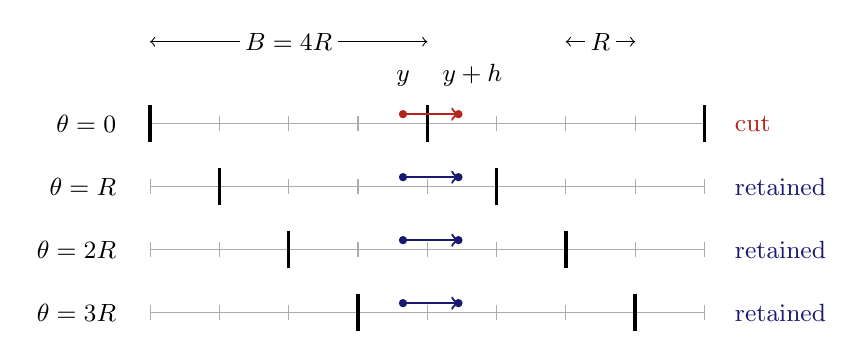
\begin{tikzpicture}[x=.88cm,y=.8cm,font=\small]
 \foreach \row/\shift/\name in {0/0/{0},1/1/{R},2/2/{2R},3/3/{3R}} {
  \begin{scope}[yshift=-\row*0.8cm]
   \node[anchor=east] at (-.35,0) {$\theta=\name$};
   \draw[gray!65] (0,0)--(8,0);
   \foreach \x in {0,...,8} {\draw[gray!65] (\x,-.12)--(\x,.12);}
   \ifnum\row=0
    \foreach \x in {0,4,8} {\draw[very thick] (\x,-.29)--(\x,.29);}
    \draw[->,thick,BrickRed] (3.65,.15)--(4.45,.15);
    \fill[BrickRed] (3.65,.15) circle (1.5pt);
    \fill[BrickRed] (4.45,.15) circle (1.5pt);
    \node[anchor=west,BrickRed] at (8.3,0) {cut};
   \else
    \draw[very thick] (\shift,-.29)--(\shift,.29);
    \draw[very thick] (\shift+4,-.29)--(\shift+4,.29);
    \draw[->,thick,MidnightBlue] (3.65,.15)--(4.45,.15);
    \fill[MidnightBlue] (3.65,.15) circle (1.5pt);
    \fill[MidnightBlue] (4.45,.15) circle (1.5pt);
    \node[anchor=west,MidnightBlue] at (8.3,0) {retained};
   \fi
  \end{scope}
 }
 \node[anchor=south] at (3.65,.43) {$y$};
 \node[anchor=south] at (4.65,.43) {$y+h$};
 \draw[<->] (0,1.3)--(4,1.3);
 \node[fill=white,inner sep=2pt] at (2,1.3) {$B=4R$};
 \draw[<->] (6,1.3)--(7,1.3);
 \node[fill=white,inner sep=2pt] at (6.5,1.3) {$R$};
\end{tikzpicture}

 \caption{A one-dimensional section of the shifted partitions, with
 $B=4R$ and a fixed pair $y,y+h$. Thin ticks mark the same $R$-grid in
 every row; thick ticks are the $B$-box faces. In the first row the
 translation crosses a box face and is cut. In the other three rows it
 stays inside one box. In general, only $O(H/R+1)$ of the $B/R$ shifts
 can separate a pair with $|h|\le H$. Sandwiching the averaged error
 by $W_R$ makes its expectation cost proportional to the excitation
 density, as in \eqref{mom:boundary-cost}.}
 \label{fig:shifted-grid}
\end{figure}

\subsection{The Fourier transform of the limiting density}

Each cut translation acts separately on the $B$-boxes. We may therefore
apply Proposition~\ref{mom:local-covariance} to it. The remaining
calculation identifies the Neumann-mode trace with the Fourier transform
of $F_\alpha$, defined in \eqref{en:limiting-V}.

\begin{proposition}[Momentum characteristic integrals]
\label{mom:characteristic}
For every fixed $H<\infty$,
\begin{equation}\label{mom:characteristic-limit}
 \int e^{ih\cdot p}\,\dd\mathfrak m_\Phi(p)
     =\int_{\R^3}e^{ih\cdot p}F_\alpha(p)
                          \frac{\dd p}{(2\pi)^3}+o(1),
 \qquad |h|\le H.
\end{equation}
The error is uniform in $h$ and in normalized, possibly complex,
ground vectors, with the iterated-limit convention of
Section~\ref{set:section}.
\end{proposition}

\begin{proof}
Fix a shifted partition $\mathcal C$. In local coordinates $[0,B)^3$,
the restriction of $T_h^{\mathcal C}$ is the contraction
\[
 (C_{b,h}g)(y)=\1_{[0,B)^3}(y+h)g(y+h).
\]
It is identical in every box. Write $W$ for the restriction of $W_R$
to a box, and $e_p$ for its normalized Neumann cosine mode with
$p\in(\pi/B)\N_0^3$. Proposition~\ref{mom:local-covariance}, including
its complex-contraction assertion, gives
\begin{equation}\label{mom:local-translation-trace}
 \frac1V\langle\dd\Gamma(W_RT_h^{\mathcal C}W_R)\rangle_\Phi
  =\frac1{B^3}\sum_{p\ne0}
        \langle e_p,WC_{b,h}We_p\rangle F_\alpha(p)+o(1).
\end{equation}
The estimate applies uniformly to these shifted grids: simultaneous
translation maps the ground space unitarily to itself, and the local
bound is uniform over its normalized vectors.

We compute the diagonal on a fixed annulus
$0<\delta\le|p|\le J$. At least one coordinate has
$|p_i|\ge\delta/\sqrt3$. The mean of its cosine over an $R$-interval
is bounded by $2/(R|p_i|)$, whereas each other cosine mean has absolute
value at most one. Including the Neumann normalization factors and
summing the squared cell means gives
\[
 \|(1-W)e_p\|\le\frac{C}{\delta R}.
\]
Since $C_{b,h}$ is a contraction,
\begin{equation}\label{mom:Neumann-diagonal}
 \langle e_p,WC_{b,h}We_p\rangle
   =\prod_{i=1}^3\cos(p_i h_i)
                  +O\left(\frac1{\delta R}+\frac HB\right).
\end{equation}
To verify the translation term, extend the cosine formula for $e_p$
to $\R^3$. Removing the clipping changes its integral by $O(H/B)$:
the boundary layer has relative volume $O(H/B)$ and
$|e_p(y)e_p(y+h)|\le C/B^3$. On the full box the integral factors.
For $p_i>0$, the sine--cosine integral over $[0,B]$ is zero because
$p_iB\in\pi\N$; the cosine-square integral gives $\cos(p_i h_i)$.
For $p_i=0$ the factor is one.

Uniformly for $\alpha\in I_\alpha$, the explicit formula gives
\begin{equation}\label{mom:profile-majorant}
 F_\alpha(p)\le C\min(|p|^{-1},|p|^{-4}).
\end{equation}
The normalized Neumann-lattice tails in \eqref{en:lattice-tails}
therefore bound the contributions of $0<|p|\le\delta$ and $|p|\ge J$
by $C\delta^2$ and $C/J$, respectively, uniformly in $B$, for
$0<\delta<1<J$. The same bounds hold for the corresponding integrals.

We can now truncate \eqref{mom:local-translation-trace} to a fixed
annulus, use \eqref{mom:Neumann-diagonal}, and take Riemann sums.
The Neumann mesh has density $\pi^{-3}$ in the nonnegative octant.
On the annulus the integrands are bounded and equicontinuous for
$|h|\le H$ and $\alpha\in I_\alpha$; continuous cutoffs at its edges
may be used. Letting $\delta\downarrow0$ and $J\uparrow\infty$ after
these estimates yields, uniformly in $h$ and $\mathcal C$,
\begin{align}
 \frac1V\langle\dd\Gamma(W_RT_h^{\mathcal C}W_R)\rangle_\Phi
 &=\frac1{\pi^3}\int_{[0,\infty)^3}
       F_\alpha(p)\prod_i\cos(p_i h_i)\,\dd p+o(1)\notag\\
 &=\int_{\R^3}F_\alpha(p)e^{ih\cdot p}
                          \frac{\dd p}{(2\pi)^3}+o(1).
 \label{mom:octant-Fourier}
\end{align}
The last equality uses reflection symmetry in each coordinate.
Averaging over $\mathcal C$ and applying
\eqref{mom:remove-coarse} and \eqref{mom:boundary-cost} proves
\eqref{mom:characteristic-limit}.
\end{proof}

\subsection{Physical units and bounded continuous tests}

The characteristic integrals include the total mass by taking $h=0$.
Fourier inversion will first give compact-test convergence. Together
with total mass convergence and positivity, this controls the momentum
tails and allows arbitrary bounded continuous test functions.

\begin{proof}[Proof of Theorem~\ref{thm:main}]
Fix $a>0$. For a sufficiently small density $\rho>0$, put
$\eta=\rho a^3$ and
\begin{equation}\label{asm:physical-scale}
 s_* =\sqrt{\frac{\alpha_0}{\rho a}},\qquad
 D_* =\rho s_*^3=\frac{\alpha_0^{3/2}}{\sqrt\eta}.
\end{equation}
Choose $R,B$ from this $D_*$ by \eqref{set:nested-lengths}.
For any thermodynamic sequence $N_k,L_k\to\infty$ with
$N_k/L_k^3\to\rho$, let $K_k$ be a positive multiple of $B$ nearest
to $L_k/s_*$. Set
\[
 s_k=L_k/K_k,\qquad r_k=a/s_k,\qquad
 D_k=N_k/K_k^3,\qquad \alpha_k=D_kr_k.
\]
Then $K_k\to\infty$, $s_k\to s_*$, $D_k\to D_*$, and
$\alpha_k\to\alpha_0$. Thus all the nested partitions and parameter
conditions hold on the tail of every such sequence.

The unitary change of variables is
\begin{equation}\label{asm:unitary-scaling}
 (U_k\Psi)(y_1,\ldots,y_{N_k})
       =s_k^{3N_k/2}\Psi(s_ky_1,\ldots,s_ky_{N_k}).
\end{equation}
It maps the allowed sets and form domains to their scaled versions,
with $q_{K_k,r_k}[U_k\Psi]=s_k^2q_{L_k,a}[\Psi]$, and hence maps
ground eigenspaces unitarily. The corresponding one-particle unitary
sends a physical plane wave of momentum $\kappa$ to the scaled one
of momentum $p=s_k\kappa$, preserving its occupation. Also
\begin{equation}\label{asm:gas-identity}
 D_kr_k^3=(N_k/L_k^3)a^3\longrightarrow\eta,
 \qquad D_k\sqrt\eta\longrightarrow\alpha_0^{3/2}.
\end{equation}

Suppress $k$ temporarily. For a normalized physical ground vector
$\Psi$, put $\Phi=U\Psi$ and
\begin{equation}\label{mom:physical-measure}
 \lambda=s\sqrt{8\pi\rho a},\qquad
 \sigma_\Psi=\frac1{D\sqrt\eta}
                  (p\mapsto p/\lambda)_*\mathfrak m_\Phi.
\end{equation}
The normalized momentum sum in \eqref{intro:main-limit}, evaluated in
the pure state $|\Psi\rangle\langle\Psi|$, is
$\int f\,\dd\sigma_\Psi$. In the inner limit,
$\lambda\to\lambda_0:=\sqrt{8\pi\alpha_0}$.
The target measure $\sigma_0:=\nu_{\mathrm{Bog}}$ from
\eqref{intro:profile} satisfies
\begin{equation}\label{mom:target-measure}
 \sigma_0=(p\mapsto p/\lambda_0)_*
       \left(\alpha_0^{-3/2}F_{\alpha_0}(p)
                                    \frac{\dd p}{(2\pi)^3}\right).
\end{equation}
This follows by substituting $p=\sqrt{8\pi\alpha_0}\,t$ in the
explicit formula \eqref{en:limiting-V}.

Apply Proposition~\ref{mom:characteristic} at $h/\lambda$ and use
\eqref{asm:gas-identity}. Since $\lambda$ stays bounded away from
zero, we obtain
\begin{equation}\label{mom:physical-characteristic}
 \int e^{ih\cdot t}\,\dd\sigma_\Psi(t)
       =\int e^{ih\cdot t}\,\dd\sigma_0(t)+o(1),
\end{equation}
uniformly on each compact set of $h$ and uniformly over the ground
vectors. Replacing $\alpha,\lambda$ in the continuous integral by
their inner limits costs only an inner-limit error: the majorant in
\eqref{mom:profile-majorant} is integrable, and truncation in $p$ makes
this replacement uniform on compact $h$-sets. The case $h=0$ gives
total mass convergence and, in particular, a uniform mass bound in
the iterated limit.

For $g\in C_c^\infty(\R^3)$, Fourier inversion and its integrable
Fourier transform imply
\[
 \int g\,\dd(\sigma_\Psi-\sigma_0)=o(1).
\]
Indeed, on a fixed compact Fourier set use
\eqref{mom:physical-characteristic}; on its complement use the mass
bound times the $L^1$ tail of the Fourier transform. Uniform
approximation and the same mass bound give this conclusion for all
$g\in C_c(\R^3)$.

Now let $f$ be any bounded continuous real function. Choose
$\chi\in C_c^\infty(\R^3)$ with $0\le\chi\le1$ and
$\int(1-\chi)\,\dd\sigma_0$ as small as desired. Positivity gives
\begin{align}
 \left|\int f\,\dd(\sigma_\Psi-\sigma_0)\right|
 &\le\left|\int f\chi\,\dd(\sigma_\Psi-\sigma_0)\right|\notag\\
 &\quad+\|f\|_\infty\left\{
       2\int(1-\chi)\,\dd\sigma_0
       +|\sigma_\Psi(\R^3)-\sigma_0(\R^3)|
       +\left|\int\chi\,\dd(\sigma_\Psi-\sigma_0)\right|\right\}.
 \label{mom:tightness}
\end{align}
The compact tests and the mass difference tend to zero in the stated
iterated sense. For a prescribed $\eps>0$, first choose $\chi$ and
the compact-test approximations, then choose the auxiliary parameters
and a lower threshold on $D_*$. Equation~\eqref{asm:physical-scale}
turns that threshold into $\rho_0(a,f,\eps)>0$. It works for every
fixed $0<\rho<\rho_0$ and every density-convergent thermodynamic
sequence. The volume threshold may depend on that fixed density and
sequence; no convergence rate for $N_k/L_k^3$ is required.

Finally, Lemma~\ref{set:ground-space} makes every finite-volume ground
eigenspace finite dimensional. Each state in $\mathcal G_{N,L,a}$
has a spectral decomposition
$\Gamma=\sum_b\omega_b|\Psi_b\rangle\langle\Psi_b|$ with
normalized ground vectors, $\omega_b\ge0$, and $\sum_b\omega_b=1$.
Its momentum measure is $\sum_b\omega_b\sigma_{\Psi_b}$. The absolute
error for $f$ is therefore at most the largest pure-state error at
that volume. All preceding bounds were uniform in the pure ground
vector, so the conclusion holds with the supremum over
$\Gamma\in\mathcal G_{N,L,a}$ required by the theorem.
\end{proof}

\begin{thebibliography}{99}

\bibitem{BBCOS}
G.~Basti, M.~Brooks, S.~Cenatiempo, A.~Olgiati, and B.~Schlein,
\emph{The Lee--Huang--Yang energy for a dilute gas of hard spheres:
an upper bound}, preprint (2026),
\href{https://arxiv.org/abs/2603.13084v2}{arXiv:2603.13084v2}.

\bibitem{BBCOSgeneral}
G.~Basti, M.~Brooks, S.~Cenatiempo, A.~Olgiati, and B.~Schlein,
\emph{Lee--Huang--Yang Energy for Dilute Bose Gases:
an Upper Bound for General Potentials}, preprint (2026),
\href{https://arxiv.org/abs/2609.25314v1}{arXiv:2609.25314v1}.

\bibitem{BCGOPS}
G.~Basti, S.~Cenatiempo, A.~Giuliani, A.~Olgiati, G.~Pasqualetti,
and B.~Schlein,
\emph{Upper Bound for the Ground State Energy of a Dilute Bose Gas
of Hard Spheres}, Arch. Ration. Mech. Anal. \textbf{248} (2024),
article~100.
\href{https://doi.org/10.1007/s00205-024-02049-w}{doi:10.1007/s00205-024-02049-w}.

\bibitem{BCS2021}
G.~Basti, S.~Cenatiempo, and B.~Schlein,
\emph{A new second-order upper bound for the ground state energy
of dilute Bose gases}, Forum Math. Sigma \textbf{9} (2021), e74.
\href{https://doi.org/10.1017/fms.2021.66}{doi:10.1017/fms.2021.66}.

\bibitem{BPP}
I.~Benjamini, R.~Pemantle, and Y.~Peres,
\emph{Unpredictable paths and percolation},
Ann. Probab. \textbf{26} (1998), no.~3, 1198--1211.
\href{https://doi.org/10.1214/aop/1022855749}{doi:10.1214/aop/1022855749}.

\bibitem{BBCS}
C.~Boccato, C.~Brennecke, S.~Cenatiempo, and B.~Schlein,
\emph{Bogoliubov theory in the Gross--Pitaevskii limit},
Acta Math. \textbf{222} (2019), no.~2, 219--335.
\href{https://doi.org/10.4310/ACTA.2019.v222.n2.a1}{doi:10.4310/ACTA.2019.v222.n2.a1}.

\bibitem{Bogoliubov}
N.~N.~Bogoliubov,
\emph{On the theory of superfluidity},
J. Phys. (USSR) \textbf{11} (1947), no.~1, 23--32.

\bibitem{BLN}
C.~Brennecke, J.~Lee, and P.~T.~Nam,
\emph{Second Order Expansion of Gibbs State Reduced Density Matrices
in the Gross--Pitaevskii Regime}, SIAM J. Math. Anal. \textbf{56}
(2024), no.~4, 5262--5284.
\href{https://doi.org/10.1137/23M1608215}{doi:10.1137/23M1608215}.
Numbered locators refer to
\href{https://arxiv.org/abs/2310.05448v2}{arXiv:2310.05448v2}.

\bibitem{CJL}
E.~A.~Carlen, I.~Jauslin, and E.~H.~Lieb,
\emph{Analysis of a Simple Equation for the Ground State of the Bose Gas II:
Monotonicity, Convexity, and Condensate Fraction},
SIAM J. Math. Anal. \textbf{53} (2021), no.~5, 5322--5360.
\href{https://doi.org/10.1137/20M1376820}{doi:10.1137/20M1376820}.
Numbered locators refer to
\href{https://arxiv.org/abs/2010.13882v3}{arXiv:2010.13882v3}.

\bibitem{Doob}
J.~L.~Doob,
\emph{Conditional Brownian motion and the boundary limits of harmonic
functions}, Bull. Soc. Math. France \textbf{85} (1957), 431--458.
\href{https://doi.org/10.24033/bsmf.1494}{doi:10.24033/bsmf.1494}.

\bibitem{Dyson}
F.~J.~Dyson,
\emph{Ground-State Energy of a Hard-Sphere Gas},
Phys. Rev. \textbf{106} (1957), no.~1, 20--26.
\href{https://doi.org/10.1103/PhysRev.106.20}{doi:10.1103/PhysRev.106.20}.

\bibitem{Fournais2021}
S.~Fournais,
\emph{Length scales for BEC in the dilute Bose gas},
in \emph{Partial Differential Equations, Spectral Theory, and Mathematical Physics:
The Ari Laptev Anniversary Volume}, EMS Series of Congress Reports~18,
EMS Press, 2021, 115--133.
\href{https://doi.org/10.4171/ECR/18-1/7}{doi:10.4171/ECR/18-1/7}.

\bibitem{FJGMOT}
S.~Fournais, L.~Junge, T.~Girardot, L.~Morin, M.~Olivieri, and A.~Triay,
\emph{The free energy of dilute Bose gases at low temperatures interacting
via strong potentials},
\href{https://arxiv.org/abs/2408.14222v1}{arXiv:2408.14222v1} (2024).
Published in Ann. Henri Poincar\'e (2026),
\href{https://doi.org/10.1007/s00023-026-01676-1}{doi:10.1007/s00023-026-01676-1}.
Numbered locators in this paper refer to the cited arXiv version.

\bibitem{FS2020}
S.~Fournais and J.~P.~Solovej,
\emph{The energy of dilute Bose gases},
Ann. of Math. (2) \textbf{192} (2020), no.~3, 893--976.
\href{https://doi.org/10.4007/annals.2020.192.3.5}{doi:10.4007/annals.2020.192.3.5}.

\bibitem{FS2023}
S.~Fournais and J.~P.~Solovej,
\emph{The energy of dilute Bose gases II: the general case},
Invent. Math. \textbf{232} (2023), no.~2, 863--994.
\href{https://doi.org/10.1007/s00222-022-01175-0}{doi:10.1007/s00222-022-01175-0}.

\bibitem{HHNST}
F.~Haberberger, C.~Hainzl, P.~T.~Nam, R.~Seiringer, and A.~Triay,
\emph{The free energy of dilute Bose gases at low temperatures},
preprint (2023),
\href{https://arxiv.org/abs/2304.02405v2}{arXiv:2304.02405v2} (2024).

\bibitem{Jauslin2024}
I.~Jauslin,
\emph{The Simplified Approach to the Bose Gas Without Translation
Invariance}, J. Stat. Phys. \textbf{191} (2024), article~88.
\href{https://doi.org/10.1007/s10955-024-03299-4}{doi:10.1007/s10955-024-03299-4}.

\bibitem{Junge2026}
L.~Junge,
\emph{Propagation of Condensation via Neumann Localization in the
Dilute Bose Gas}, preprint (2026),
\href{https://arxiv.org/abs/2603.20776v1}{arXiv:2603.20776v1}.

\bibitem{LHY}
T.~D.~Lee, K.~Huang, and C.~N.~Yang,
\emph{Eigenvalues and Eigenfunctions of a Bose System of Hard Spheres
and Its Low-Temperature Properties},
Phys. Rev. \textbf{106} (1957), no.~6, 1135--1145.
\href{https://doi.org/10.1103/PhysRev.106.1135}{doi:10.1103/PhysRev.106.1135}.

\bibitem{LS2002}
E.~H.~Lieb and R.~Seiringer,
\emph{Proof of Bose--Einstein Condensation for Dilute Trapped Gases},
Phys. Rev. Lett. \textbf{88} (2002), 170409.
\href{https://doi.org/10.1103/PhysRevLett.88.170409}{doi:10.1103/PhysRevLett.88.170409}.

\bibitem{LSY2005}
E.~H.~Lieb, R.~Seiringer, and J.~Yngvason,
\emph{Justification of $c$-Number Substitutions in Bosonic Hamiltonians},
Phys. Rev. Lett. \textbf{94} (2005), 080401.
\href{https://doi.org/10.1103/PhysRevLett.94.080401}{doi:10.1103/PhysRevLett.94.080401}.

\bibitem{LS2001}
E.~H.~Lieb and J.~P.~Solovej,
\emph{Ground State Energy of the One-Component Charged Bose Gas},
Comm. Math. Phys. \textbf{217} (2001), 127--163.
\href{https://doi.org/10.1007/s002200000353}{doi:10.1007/s002200000353}.

\bibitem{LY}
E.~H.~Lieb and J.~Yngvason,
\emph{Ground State Energy of the Low Density Bose Gas},
Phys. Rev. Lett. \textbf{80} (1998), no.~12, 2504--2507.
\href{https://doi.org/10.1103/PhysRevLett.80.2504}{doi:10.1103/PhysRevLett.80.2504}.

\bibitem{H}
OpenAI,
\emph{Ground-state condensation in the dilute hard-sphere gas},
OpenAI Math Release preprint
\href{https://github.com/openai/math/blob/main/preprints/Ground-state-condensation-in-the-dilute-hard-sphere-gas-September-24-2026/paper.pdf}{OAI:Ground-state-condensation-in-the-dilute-hard-sphere-gas-September-24-2026},
2026.

\bibitem{Timar}
\'A.~Tim\'ar,
\emph{Boundary-connectivity via graph theory},
Proc. Amer. Math. Soc. \textbf{141} (2013), no.~2, 475--480.
\href{https://doi.org/10.1090/S0002-9939-2012-11333-4}{doi:10.1090/S0002-9939-2012-11333-4}.
Theorem locators refer to
\href{https://arxiv.org/abs/0711.1713v2}{arXiv:0711.1713v2}.

\bibitem{YY}
H.-T.~Yau and J.~Yin,
\emph{The Second Order Upper Bound for the Ground Energy of a Bose Gas},
J. Stat. Phys. \textbf{136} (2009), 453--503.
\href{https://doi.org/10.1007/s10955-009-9792-3}{doi:10.1007/s10955-009-9792-3}.

\end{thebibliography}

\end{document}
